% !TeX encoding = UTF-8
% !TeX program = pdflatex
% !TeX spellcheck = en_US
\documentclass[binding=0.6cm,noexaminfo]{sapthesis}

\usepackage{microtype}
\usepackage[english]{babel}
\usepackage[utf8]{inputenc}
\usepackage{hyperref}

\usepackage{graphicx}
\graphicspath{{./images/}}

\usepackage{mathtools}
\usepackage{amssymb}
\usepackage{subcaption}
\usepackage{multirow}

\usepackage{tabularx}

\hypersetup{pdftitle={3D Indoor Environment Reconstruction using Wi-Fi Sensing}, pdfauthor={Matteo Orsini}}

\title{3D Indoor Environment Reconstruction using Wi-Fi Sensing}
\author{Matteo Orsini}
\IDnumber{1795119}
\course{Computer Science Master Degree}
\courseorganizer{Faculty of Information Engineering, Informatics, and Statistics}
\AcademicYear{2021/2022}
\advisor{Prof. Luigi Cinque}
\coadvisor{Prof. Danilo Avola}
\coadvisor{Dr. Marco Cascio}
\authoremail{orsini.matteo99@gmail.com}
\copyyear{2022}
\thesistype{Tesi di Laurea Magistrale}

\begin{document}
\frontmatter
\maketitle

\begin{acknowledgments}
Vorrei dedicare questo spazio a coloro che hanno contribuito alla realizzazione di questo lavoro.
\\\\
Grazie a tutta la mia famiglia. In particolare, ai miei genitori che da sempre mi sostengono e supportano durante la realizzazione dei miei progetti. Inoltre, un enorme ringraziamento ai miei nonni materni che mi hanno sempre aiutato, e un pensiero va anche ai miei nonni paterni che prematuramente mi hanno lasciato.
\\\\
Un sentito grazie a Fabrizio, con il quale ho condiviso questo percorso di laurea passo dopo passo. Inoltre, un ringraziamento a tutti gli amici, in particolare a Christian, Gianluca, Mina e Emanuele.
\\\\
Grazie al mio relatore, Prof. Luigi Cinque, che mi ha offerto la possibilità di dedicarmi a questo lavoro. Ringraziamenti d'obbligo al Prof. Danilo Avola e al Dott. Marco Cascio, i quali mi hanno motivato e supportato per tutta la durata di questo lavoro.
\end{acknowledgments}

\tableofcontents
\mainmatter

\chapter{Introduction}

This chapter will introduce the aim and scope of this thesis in Section \ref{sec:aim-scope}. Then, in Section \ref{sec:sota} the state of the art regarding the topic of this thesis will be presented. Finally, in Section \ref{sec:contribution-outline} the contributions of this work and the structure of this document are highlighted.

\section{Aim and Scope}\label{sec:aim-scope}
% WiFi diffusion
Initially, Wi-Fi was introduced to enable wireless connection to desktops, laptops and mobile devices and provide network connectivity among them. The subsequent diffusion of Internet of Things (IoT) allowed an exponential growth of commodity Wi-Fi devices and the diffusion of ubiquitous Wi-Fi coverage in both private and public places.
% Wi-Fi based sensing applications
These devices allowed researchers to widen the purposes of Wi-Fi from just providing network communication to enabling the so-called Wi-Fi sensing applications, which use the Wi-Fi signal in order to sense the surrounding physical environment and perform various tasks.

% Pro and cons of these applications
Wi-Fi sensing can be employed in several scenarios, in fact it is not only limited to indoor environments but it is also possible to exploit public Wi-Fi signals to enable outdoor purposes. Moreover, in contrast to video-based systems, Wi-Fi sensing doesn't require Line-of-Sight (LOS) when collecting information about the physical environment, since signal can propagate to the destination following various paths, phenomenon known as multipath effect. In addition, Wi-Fi is not affected by light conditions or visual occlusions like video systems and it can also operate with very cheap commodity devices, contrary to video applications which may require very expensive cameras if high quality images are required.

% Task description
Several tasks have been addressed in the literature employing Wi-Fi sensing techniques, like health monitoring \cite{wifall}, activity classification \cite{human-to-human}, pose estimation \cite{person-in-wifi, towards-human-pose-construction, wimose}, gesture recognition \cite{novel-gesture-recognition} and through the wall sensing \cite{through-wall-sensing, violating-privacy}. At the moment of writing, reviewing the state of the art, this is the first work which aims to produce a 3D reconstruction of the environment only relying on the Wi-Fi signal collected in it.
% Motivazione
In fact, the environment is one of the elements that affects most the Wi-Fi signal during its propagation \cite{effects-housing-environments, carm}. The propagation of the signal is even impacted by the different materials which the objects in the environment are made of. In detail, each material affects the signal strength in a particular way due to different interactions with the propagated signal and the electrical properties of that material. For instance, metal is a significant contributor in signal strength fluctuations, since it scatters the signal in many directions. Instead, isolators (like wood and plastic) may contribute to the reduction of the signal strength based on the object thickness and the signal wavelength \cite{study-materials-on-wifi}.
One of the major reasons that motivate this work is to provide new insights regarding the information that the Wi-Fi signal actually carries and we can extract from it. Moreover, a system able to reconstruct the environment can be incredibly useful in scenarios like natural disasters or when an environment is not accessible in a safe way by a person. Using technologies already available, it could provide a view of the environment and offer the possibility to plan accordingly how to move around the obstacles by an autonomous machine or a specialized person.

% Descrizione setup per esperimenti?
This work will focus on the reconstruction of the environment considering single rooms. In order to gather information about the environment it is possible to use the Received Signal Strength Indicator (RSSI) or the Channel State Information (CSI) measurements \cite{tool-release} which are collected from the Wi-Fi signal exchanged between a transmitting (TX) and a receiving (RX) antenna. This work will rely on CSI measurements which are generally used for Wi-Fi sensing applications since they are more stable and provide more information than RSSI, both of them will be analyzed in depth in Chapter \ref{cap:wireless-chapter}.

Instead, regarding the 3D reconstruction, there are several methods that are used in the literature to represent 3D objects \cite{3d-repr-survey}: in Figure \ref{fig:3d-repr} are shown some of the most popular among them. Typically, objects are represented as a 3D surface composed by a triangular mesh, or more in general a polygonal mesh. Another representation is point clouds which represent an object as a set of data points in the space. Finally, another representation is in voxel space, the one adopted in this work, that approximates objects as voxels, the natural extension of pixels in a 3-dimensional space.

\begin{figure}[h!]
\centering
\begin{subfigure}{.32\textwidth}
	\centering
	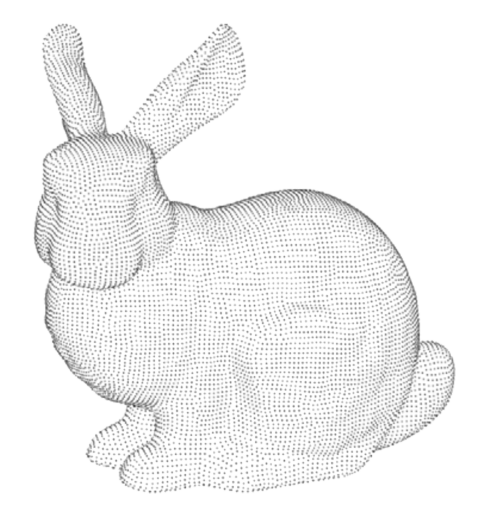
\includegraphics[width=\linewidth]{bunny-point}
	\caption{}
\end{subfigure}
\begin{subfigure}{.32\textwidth}
	\centering
	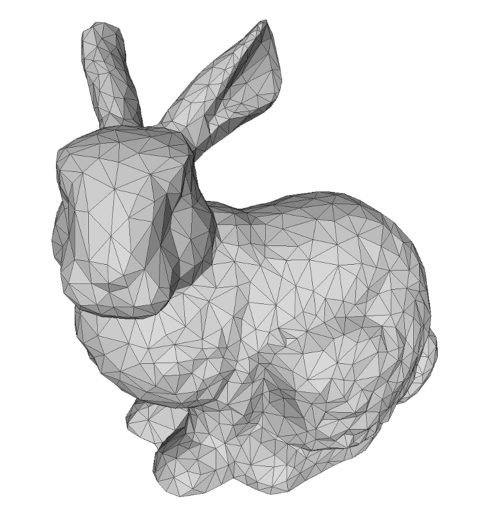
\includegraphics[width=\linewidth]{bunny-mesh}
	\caption{}
\end{subfigure}
\begin{subfigure}{.32\textwidth}
	\centering
	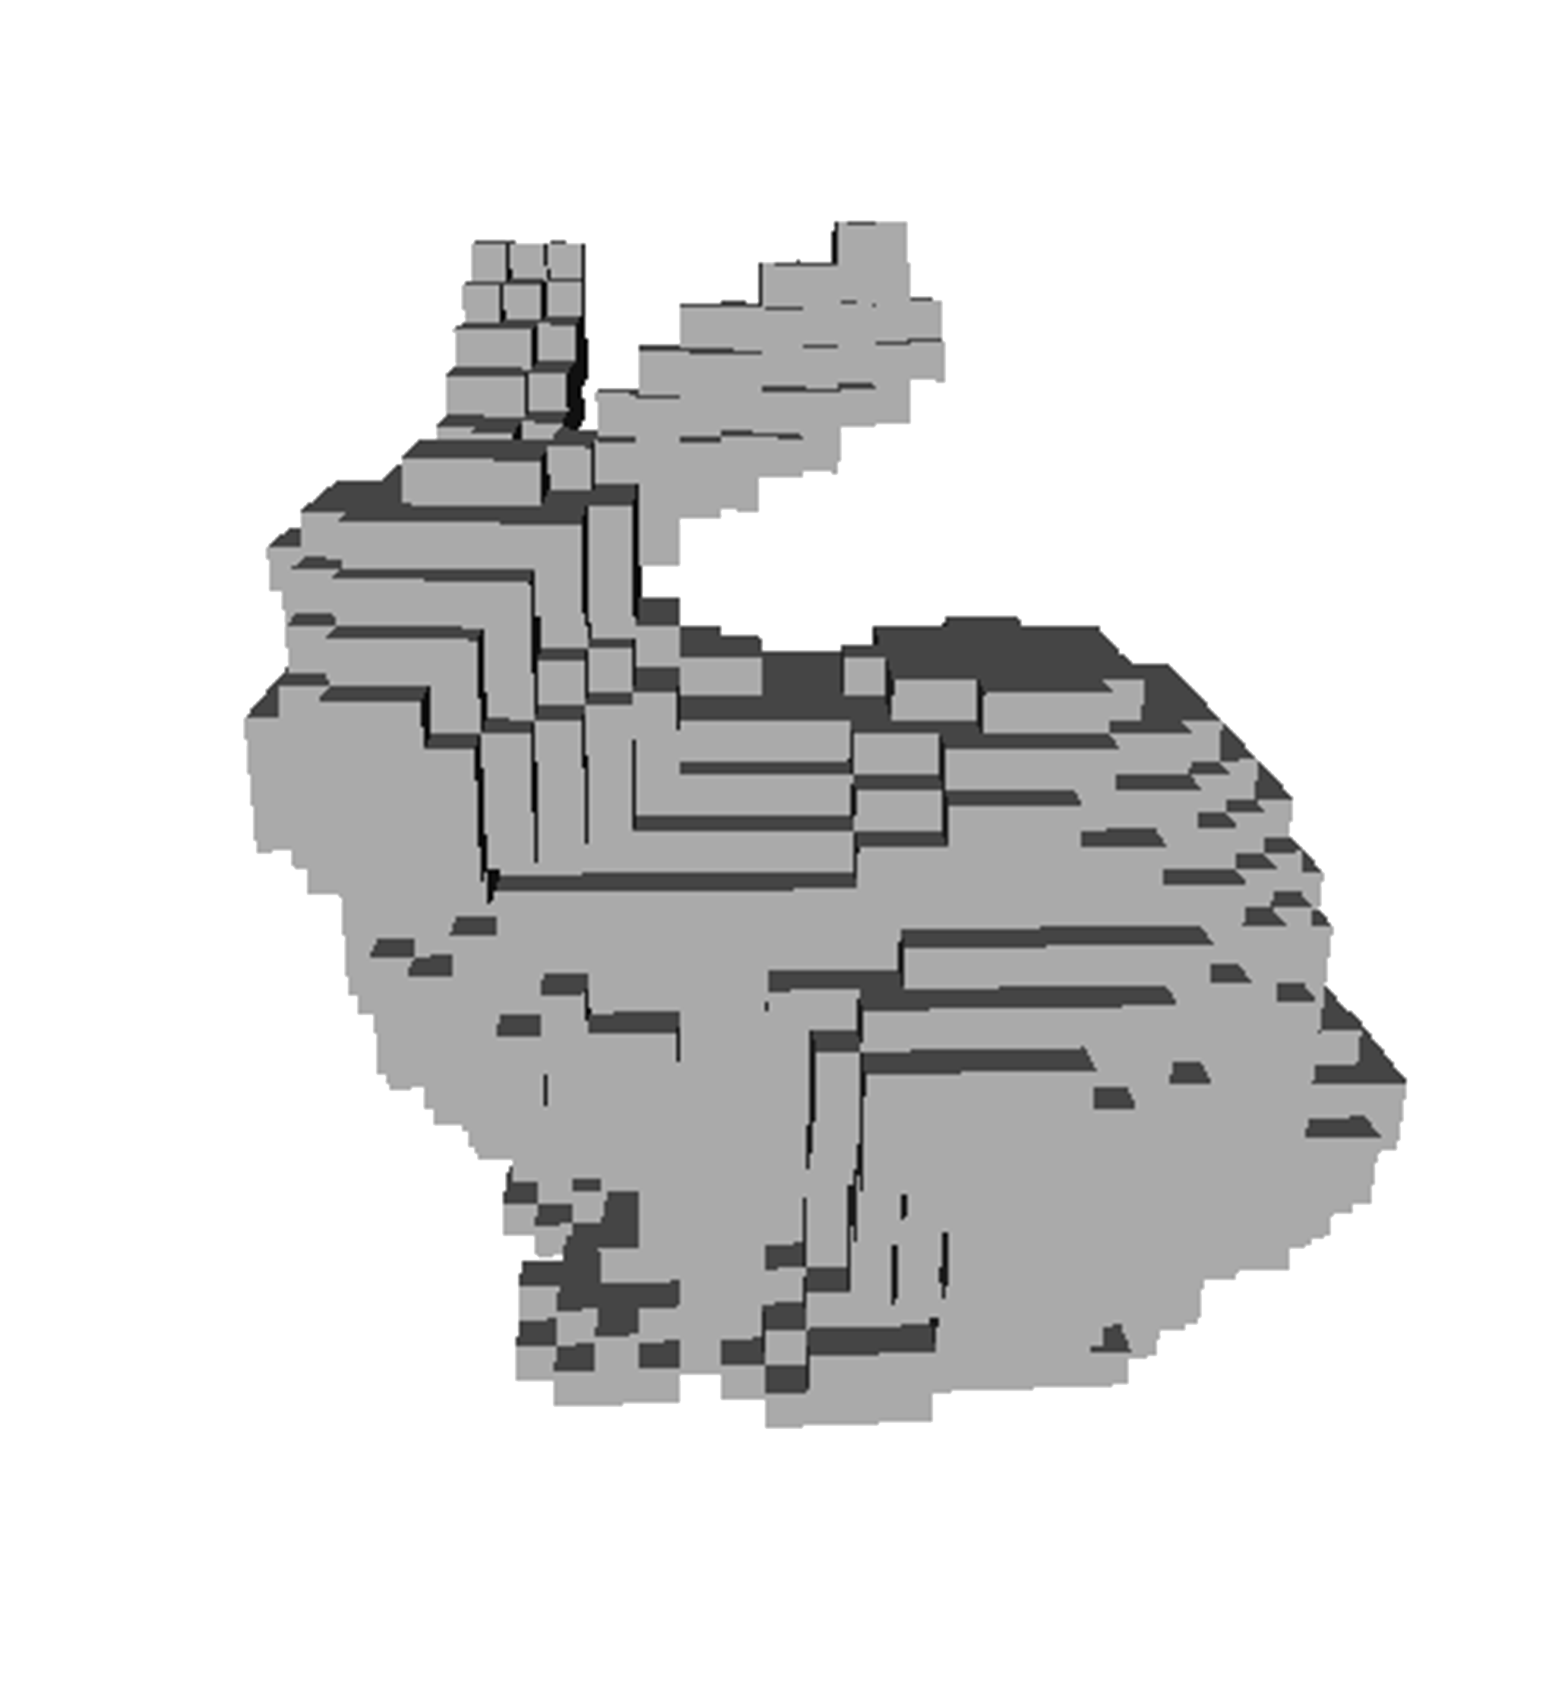
\includegraphics[width=\linewidth]{bunny-voxel}
	\caption{}
\end{subfigure}
\caption{Different representations for a 3D object. Point cloud representation (a), triangular mesh representation (b) and voxel space representation (c).}
\label{fig:3d-repr}
\end{figure}

\section{State of the Art}\label{sec:sota}
% Review dei lavori precedenti in merito, principalmente ai primi lavori in campo di wifi sensing
In the following section is illustrated the state of the art for both Wi-Fi sensing tasks and 3D reconstruction tasks. The two fields are reviewed separately, since there are no papers already available which produce an extensive study on both topics at the same time in relation to the environment.

\subsection{Wi-Fi Sensing}

The field of Wi-Fi Sensing is relatively new: even if the protocols currently used were already present in the IEEE 802.11a standard, only in the last few years the potential of this technology was acknowledged and researchers started to focus more on this topic \cite{white-paper-wifi-sensing}.

Wi-Fi sensing methods can be categorized in two major classes: RSSI and CSI based approaches. As stated before, CSI is generally more used in the context of Wi-Fi sensing since it is more stable and provides more information than RSSI.

% RSSI
Starting from RSSI methods, in \cite{3d-imaging-sparse-wireless-signal-reconstruction-ml}, a shape of an unknown object is reconstructed using the RSSI measure and relying on machine learning techniques. This work focuses mainly on the denoising of the dataset but it shows how even using RSSI we can obtain enough information to perform a 3D reconstruction of a single simple object.

% CSI
Regarding CSI-based approaches, the release of tools able to extract CSI measurements from commodity devices was extremely important in the field \cite{tool-release}. In fact, early works used custom hardware which wasn't largely available to the public.
In detail, CSI is collected for each transmitter-receiver antenna pair, and it is composed by $P \times K$ complex values, where $P$ is the number of packets exchanged between the two devices and $K$ is the number of subcarriers. Then, for each complex value it is possible to extract the measured amplitude attenuation and phase shift, and use them in order to address a given task \cite{wifi-sensing-survey}.
The majority of papers using CSI-based approaches consider the CSI data as an image, called CSI image. The use of CSI images allows researchers to exploit methods already studied in the Computer Vision field for images, like Convolutional Neural Networks (CNNs), especially suited for this kind of data.

In practice, CSI images are usually redefined from each work based on the task they want to address and the kind of processing they perform on the CSI data. For example, in \cite{cnn-wifi-localization} they use CSI images for indoor localization of a mobile device in an environment. The authors define CSI images using 3 receiving antennas as an RGB image where the first channel is the amplitude of the first antenna, the second channel is the phase difference between the first and second antenna and finally the third channel is composed by the phase difference between the second and third antenna.

Another paper that performs indoor localization is \cite{cifi}. In this work the authors use the CSI data to estimate the Angle Of Arrival (AOA) of the packets and then use this data to compose what they call CSI AOA images, which are then used in order to train a deep model.

Another use of the CSI image can be seen in \cite{csi2image} which is very similar to this work. The authors try to reconstruct an image starting from CSI data using a Generative Adversarial Network (GAN). They also test their model for material sensing and device-free user localization of a single user who stays in a particular location, achieving high accuracy.

In the following other approaches based on CSI data are presented, starting from \cite{person-in-wifi} which focuses on the pose estimation problem. The aim of this task is to reconstruct the skeleton of people present in a delimited area, in this case using only Wi-Fi signal. In this work CSI images are not explicitly used, in fact the number of packets and subcarriers are merged in a single dimension of the CSI tensor in input to the model. The model is mainly composed by convolutions and produces three different outputs: a segmentation mask (SM) of the people in the scene, several heatmaps of the joints of the skeleton (JHMs) and other heatmaps called Part Affinity Fields (PAFs) that encode pairwise relationships between body parts, introduced in the popular framework Open Pose \cite{open-pose}. In the last step, the three outputs are finally merged together in order to construct the skeleton of the people in the scene.

Another work about pose estimation is the framework WiPose \cite{towards-human-pose-construction}, in which they pay particular attention to encode the prior knowledge of human skeleton into the posture construction process to ensure that the estimated joints satisfy the skeletal structure of the human body. CSI data is used also in this work after a step of data denoising and segmentation of the signal in small segments in order to train a deep model. In this paper, the data collected is fed first into a CNN to extract spatial features and then processed by a Long Short Term Memory (LSTM) which is used to handle sequential data and capture relatively long movements in the skeleton.

Regarding pose estimation the framework Wi-Mose \cite{wimose} proposes another definition of CSI image. In fact, the authors decided to fuse amplitude and phase into the CSI image, in order to provide both pose and position information. Compared to the WiPose framework, cited before, this system can work with less antennas and provides more accurate predictions.
Furthermore, a work which tried to take the Wi-Fi sensing field another step forward is the framework Wi2Vi \cite{wi2vi}. The aim of this paper is to generate video sequences associating variations in the Wi-Fi CSI with video frames, enabling the use of Wi-Fi sensing also for security purposes. The method used in this work is composed by three models: a CSI encoder, a so called domain translator and a frame decoder. All of them are then used in sequence to output a video frame from a CSI sample.

Another task in which Wi-Fi sensing has been applied is activity recognition: the paper \cite{human-to-human} focuses in particular on the recognition of human-to-human activities. Also in this work the concept of CSI image is used again with convolutional filters but on segments of the raw CSI signal.

Finally, regarding CSI approaches, it is worth mentioning the study \cite{novel-gesture-recognition}, in which the CSI is extracted from a smartphone and it is used to perform gesture recognition. This shows how much Wi-Fi sensing can be widely applied even to smartphones unlocking so many more applications in daily activities.

In the literature other technologies than Wi-Fi signals were also tested to perform tasks similar to the ones described above, for example FMCW radars \cite{human-through-wall, rf-based-3d-skeleton} or RFID \cite{rfid}. However, these technologies are not available as much as Wi-Fi communication devices, making them less suited for systems that wants to be highly available.

\subsection{3D Reconstruction}

Currently, 3D reconstruction of indoor environments can be divided in three categories based on the method used for data collection: single-view depth estimation, multi-view depth estimation and Simultaneous Localization and Mapping (SLAM) \cite{indoor-env-survey}. The main goal of depth estimation is to estimate the depth of image pixels in order to reflect the real 3D scene. The difference between single- and multi-view depth estimation is in the number of images provided to address this task. In the case of single-view the reconstruction is based on a single image, while for multi-view more than one image is provided. Instead, for the last data collection category, SLAM, a mapping system starts moving from an unknown location in an unknown environment to estimate its own position according to the surrounding and build meanwhile an incremental map of the environment.

Regarding 3D reconstruction of indoor environments, the state of the art focuses in particular on the semantic segmentation \cite{semantic-segmentation-rgbd-images, pointnet} and the room layout estimation \cite{360-mlc, psmnet} tasks. Even if these works operate on the environment they have a reconstruction which is severely different from the one adopted by this thesis, in fact they use a point cloud 3D representation of the environment assigning to each data point a label.

Instead, the 3D representation adopted by this work is much more similar to the one used in the following works, which address the task of 3D object reconstruction in the voxel space.

The first one is Pix2Vox \cite{pix2vox}, in which multiple images are fed in input to the same encoder, in order to produce several feature maps that will be fed to the decoder and output multiple volumes. Then, a context-aware fusion network  will merge the volumes together in a so called "fused volume". Finally, a refiner network is used to remove some imperfections and produce the final output.

Instead, in \cite{3d-r2n2} they present 3D-R2N2, which produces incrementally more refined reconstructions of the object as the network sees more views of it. The model has actually three modules: an encoder, based on a 2D-CNN, a recurrence module, based on a 3D-LSTM, and a decoder, based on a 3D-CNN.

A more complex approach is offered by \cite{multi-view-3d-transformer}, which proposes a framework based on a transformer network \cite{attention-is-all-you-need} able to achieve state of the art accuracy. The proposed model consists of a 2D-view encoder and a 3D-volume decoder. The encoder will take in input an embedding of the multi-view images and encode the relevant information among the different views using the attention mechanism. Instead, the decoder will learn to predict the final output based on global correlations of different spatial locations.

Finally, another work which uses a transformer model is \cite{3d-retr}. In this case, the encoder produces features starting from the 2D images, which will then be used by the decoder to produce voxel features. In the end, a CNN decoder will merge all the different 3D features producing a final prediction. One of major differences between the previous work and this one is the division of the input image in patches to feed to the encoder. This improvement is inspired by a particular variant of a transformer, the Vision Transformer (ViT) \cite{vit}, which is one of the proposed ways to apply transformers to visual tasks.


\section{Contribution and Thesis outline}\label{sec:contribution-outline}
This section briefly reports the contributions of this work with respect to the state of the art. The new field of indoor environment reconstruction using CSI data is presented and investigated, providing a new purpose for Wi-Fi sensing applications. A new dataset is collected to evaluate the performance of a system for this new task. Moreover, a novel architecture is designed and evaluated on the collected dataset. This model given in input a CSI image is able to produce a 3D reconstruction in voxel space of the environment in which the sample was collected. In addition, an extensive procedure about Wi-Fi data sanitization is applied to obtain robust features based on the signal amplitude and phase.

Finally, the structure of this thesis is described. In Chapter \ref{cap:wireless-chapter} the concepts about the wireless channel which enable Wi-Fi sensing are illustrated. Moreover, in Chapter \ref{cap:dl} is presented an overview of the deep learning techniques that are the foundations of the proposed method which is described in Chapter \ref{cap:method}. Moreover, a qualitative and quantitative evaluation of the results of the model are shown in Chapter \ref{cap:results}. Lastly, in the Chapter \ref{cap:conclusions} the conclusions of this thesis are reported.

\chapter{The wireless channel}\label{cap:wireless-chapter}

This chapter contains the theoretical concepts about wireless communication systems required to understand the technology used in Wi-Fi sensing. In the Sections \ref{sec:signal-prop} and \ref{sec:phy-model} the theory about the wireless channel is reported. Moreover, in Sections \ref{sec:rssi} and \ref{sec:csi} the Received Signal Strength Indicator and Channel State Information measurements are presented. Finally, the sanitization procedure required for the amplitude and phase components is described in Section \ref{sec:amp-pha}.

\section{Signal propagation in wireless communication}\label{sec:signal-prop}

In a wireless communication, an electromagnetic (EM) radiation is used to convey information from a transmitting (TX) to a receiving (RX) antenna. This radiation travels on a transmission medium, e.g. air or space, throughout a sinusoidal waveform. EM waves are obtained by the oscillations between the electric and magnetic fields producing a so-called electromagnetic field. Each EM wave is characterized by several properties, the most important are wavelength and frequency, shown in Figure \ref{fig:wave-pro}. The wavelength is computed between two adjacent crests of the wave. Instead, the frequency represents the number of oscillation cycles per second of the wave. 

\begin{figure}[h!]
\centering
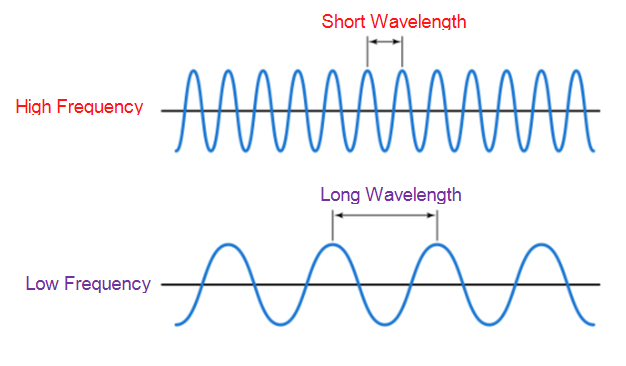
\includegraphics[width=.7\linewidth]{wave-properties}
\caption{Representation of two waves: the first with a short wavelength and an high frequency, the second with a long wavelength and a low frequency.}
\label{fig:wave-pro}
\end{figure}

A correlation between wavelength and frequency is expressed by the following equation:

\begin{equation}
v = \lambda f,
\label{eq:wlf}
\end{equation}
where $v$ is the propagation velocity, usually equals to the speed of light $c$, $\lambda$ is the wavelength measured in meters ($m$) and $f$ is the frequency measured in Hertz (Hz).
Moreover, from Eq. \ref{eq:wlf}, we can easily derive the following:

\begin{equation}
\lambda = \frac{v}{f},
\end{equation}
\begin{equation}
f= \frac{v}{\lambda},
\end{equation}
which show that frequency and wavelength are directly proportional to the propagation velocity and inversely proportional to each other.

The EM field generated from the transmission changes based on the distance from the transmitter. In particular, the area defined one wavelength or less from the TX is called near-field. Instead, the region that starts two wavelengths from the TX antenna is called far-field. In the far-field, the electric field and magnetic field at any given location are perpendicular both to each other and to the direction of propagation from the antenna.
Due to its properties, the far-field enables long-range transmissions required for most wireless sensing applications.
In response to a transmitted sinusoid $\cos 2\pi f t$, as described in \cite{wireless-communications}, we can express the electric far field at time $t$ as:

\begin{equation}
E(f, t, (r, \theta, \psi)) = \frac{\alpha_s(\theta, \psi, f) \cos 2 \pi f (t - r / c)}{r},
\label{eq:far-field}
\end{equation}
where $(r, \theta, \psi)$ is the point at which the electric field is being measured, $r$ is the distance from the transmitting antenna and $(\theta, \psi)$ are the vertical and horizontal angles from the antenna. The constant $c$ is the speed of light and $\alpha_s(\theta, \psi, f)$ is the radiation pattern of the sending antenna at frequency $f$ in the direction $(\theta, \psi)$.
If we consider a fixed receive antenna at location $u = (r, \theta, \psi)$, the previous Eq. \ref{eq:far-field} can be changed in the following way:

\begin{equation}
E_r(f, t, u) = \frac{\alpha(\theta, \psi, f) \cos 2 \pi f (t - r / c)}{r},
\label{eq:far-field-receiver}
\end{equation}
where now $\alpha(\theta, \psi, f)$ is the product of the antenna patterns of both transmit and receive antenna in the direction $(\theta, \psi)$.

Both Eqs. \ref{eq:far-field} and \ref{eq:far-field-receiver} are linear in the input, which implies that the received waveform at location $u$ in response to a weighted sum of transmitted waveforms is the weighted sum of the responses of each singular waveform.
Now, for a given $u$, we can define:

\begin{equation}
H(f) \coloneqq \frac{\alpha (\theta, \psi, f) \text{e}^{-j 2 \pi fr / c}}{r},
\end{equation}
and we have that $E_r(f, t, u) = \Re \left[ H(f) \text{e}^{j 2 \pi ft} \right]$. So, $H(f)$ is the system function for a linear time-invariant (LTI) channel, and computing its inverse Fourier transform we can obtain the impulse response.

Now, consider the case in Figure \ref{fig:signal-wall} in which we have a fixed receive antenna and a single perfectly reflecting large fixed wall. In this case we assume that the received waveform can be approximated by the sum of the free space wave from the transmitter plus the reflected free space waves from each of the reflecting obstacles.

\begin{figure}[h!]
\centering
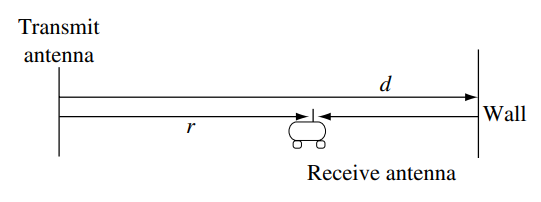
\includegraphics[width=.5\linewidth]{signal-wall}
\caption{Direct path and a reflected path.}
\label{fig:signal-wall}
\end{figure}

If we assume that the wall is very large, the reflected wave at a given point is the same (except for a sign change) as the free space wave that would exist on the opposite side of the wall if the wall was not present. This means that the reflected wave from the wall has the intensity of a free space wave at a distance equal to the distance to the wall and then back to the received antenna, i.e. $d + (d - r) = 2d - r$. The electric field is then defined for both direct and reflected wave in the following way:

\begin{equation}
E_r(f, t) = \frac{\alpha \cos 2 \pi f(t - r / c)}{r} - \frac{\alpha \cos 2 \pi f (t - (2d - r) / c)}{2d - r},
\end{equation}
where $\alpha$ is the same antenna gain for both waves. Therefore, the received signal is a superposition of two waves, both of frequency $f$.
Instead, the phase difference between the two waves is defined as follows:

\begin{equation}
\Delta\theta = \left( \frac{2 \pi f (2d - r)}{c} + \pi \right) + \left( \frac{2 \pi f r}{c} \right) = \frac{4 \pi f}{c} (d - r) + \pi.
\end{equation}

This is very important since if the phase difference is an integer multiple of $2 \pi$, the two waves add \textit{constructively}, and the received signal is strong, instead if the phase difference is an odd integer multiple of $\pi$, the two waves add \textit{destructively}, and the received signal is weak.

\section{Physical model}\label{sec:phy-model}

Previously, the signal was defined as a response to a sinusoidal input $\phi(t) = \cos 2 \pi f t$. Generalizing the definition of the signal we can take into account also the different attenuation factors that cause variations in the wireless channel strength over both time and frequency. Thus, we can define the received signal as:

\begin{equation}
y(f, t) = \sum_i a_i (f, t) \phi (t - \tau_i(f,t)),
\label{eq:phy-model-1}
\end{equation}
where $a_i(f,t)$ and $\tau_i(f,t)$ are respectively the overall attenuation and propagation delay at time $t$ from the transmitter to the receiver on path $i$. If we further assume that $a_i$ and $\tau_i$ do not depend on the frequency $f$ we can rewrite the previous equation as follows:

\begin{equation}
y(t) = \sum_i a_i (t) x(t - \tau_i(t)),
\label{eq:phy-model-2}
\end{equation}
where $x(t)$ is an arbitrary transmitted signal with non-zero bandwidth.

Since Eq. \ref{eq:phy-model-2} is linear, a fading multi-path wireless channel can be modeled with respect to time as the Channel Impulse Response (CIR) at time $t$ of a linear time-varying system, as follows:

\begin{equation}
h(\tau, t) =  \sum_i a_i (t) \delta(\tau - \tau_i(t)),
\label{eq:phy-model-3}
\end{equation}

where $\delta(\tau)$ corresponds to the Dirac delta function. By consequence, a relation between the received signal at time $t$ and an impulse $x$ transmitted at time $t - \tau$ can be established as:

\begin{equation}
y(t) = \int^{\infty}_{-\infty} h(\tau, t) x(t- \tau) d\tau.
\label{eq:phy-model-3}
\end{equation}

Next, applying the Discrete Fourier transform (DFT) to the channel impulse response, it is possible to estimate the corresponding time-varying Channel Frequency Response (CFR) defined as:

\begin{equation}
H(f;t) = \int^{\infty}_{-\infty} h(\tau, t) e^{-j2\pi f \tau} d\tau = \sum_i a_i(t) e^{-j2\pi f \tau_i(t)} = |H(f;t)| e^{j \angle H(f;t)},
\label{eq:cfr}
\end{equation}
where $|H(f;t)|$ and $\angle H(f;t)$ respectively indicate the signal amplitude and phase responses, and $j$ is the imaginary component. Instead, considering the frequency domain we can build a time-varying system as follows:

\begin{equation}
y(t) = H(f;t) x(t - \tau).
\end{equation}

However, in the case of a static environment with fixed transmit and receive antennas, the wireless channel can be described as a linear time-invariant system as follows:

\begin{equation}
h(\tau) = \sum_i a_i \delta(\tau - \tau_i),
\end{equation}

\begin{equation}
H(f) = \int^{\infty}_{-\infty} h(\tau) e^{-j2\pi f \tau} d\tau = \sum_i a_i e^{-j2\pi f \tau_i} = |H(f)| e^{j \angle H(f)},
\end{equation}
where attenuations $a_i$ and propagation delays $\tau_i$ do not change with time $t$.

The last step, for the definition of a wireless communication channel as a linear system, is to consider random factors like the noise. In fact, in the real world it is a very common factor for all communication systems since it is physical impossible to have a channel completely noise-free. The Additive White Gaussian Noise (AWGN) is usually chosen for noise modeling on the received signal. Thus, the wireless channel expressed in Eq. \ref{eq:phy-model-2} under noisy conditions can be defined as follows:

\begin{equation}
y(t) = \sum_i a_i(t) x(t - \tau_i(t)) + \omega(t),
\end{equation}
where $\omega(t)$ is the AWGN component at time $t$. In practice, this component is random and, at each time, it is drawn from a fixed zero-mean Gaussian distribution.

\section{Received Signal Strength Indicator}\label{sec:rssi}

When a signal arrives at a receive antenna is usually reduced in terms of intensity of the waveform power accumulated. In fact, the EM radiation during its propagation through the medium from the transmitter can encounter several obstacles. The Received Signal Strength Indicator (RSSI) indicates the average error associated with each received signal strength measurements \cite{rssi-def}. This measure is generally used to assess the quality of a wireless network, but its uses has been studied also for other purposes \cite{rssi-reliable}. The RSSI is expressed in decibels (dB) and it can be formally defined as follows:

\begin{equation}
PL_d = PL_{r} + 10 n \log_{10} \frac{d}{d_r} + \mathcal{N},
\end{equation}
where $PL_d$ indicates the path loss at distance $d$, $n$ the path loss exponent and $\mathcal{N}$ is a zero-mean Gaussian random variable modeling the noise. Moreover, $PL_{r}$ is the path loss at the reference distance $r$ usually computed exploiting the free-space path loss model, derived from the Friis transmission equation, which can be defined as:

\begin{equation}
FSPL = 10 \log_{10} \left( \frac{4 \pi d f}{c} \right)^2,
\end{equation}
where $d$ is the distance between the transmit and receive antenna, $c$ is the speed of light, and $f$ is the wave frequency.

\section{Channel State Information}\label{sec:csi}

In order to transmit data most wireless communications, including IEEE 802.11 Wi-Fi systems, use the Orthogonal Frequency-Division Multiplexing (OFDM) signal modulation. In OFDM, the data is transmitted in parallel using multiple spaced orthogonal subcarrier signals. Thanks to the orthogonality property of the encoding scheme, the receiver is able to recover the original signal without interference despite the overlapping sidebands.
The Channel State Information (CSI) is based on the OFDM system and offers  more fine-grained measurements than the RSSI measure for wireless systems. CSI is used to obtain information about the propagation between transmitter and receiver for each subcarrier, such as amplitude, phase, or frequency, while RSSI indicates only the relative quality of the received signal. Moreover, a time series of CSI measurements capture how wireless signal travels through surrounding objects and humans in time, frequency, and spatial domains, so it can be used for different wireless sensing applications \cite{wifi-sensing-survey}.
In a standard Wi-Fi transmission, $P$ data packets are transmitted between access points (APs). The CSI is computed for each of the $K$ OFDM-based subcarriers and related to each packet $p$ reaching the receiver.
Given $\Theta$ and $\Gamma$ representing respectively the set of transmit and receive antennas, for each subcarrier $k$ the frequency response between $\theta \in \Theta$ and $\gamma \in \Gamma$ antennas, is given by:

\begin{equation}
H(f)^{\theta, \gamma}_k = |H(f)^{\theta, \gamma}_k| e^{j \angle H(f)^{\theta, \gamma}_k},
\label{eq:h(f)}
\end{equation}
where $|H(f)^{\theta, \gamma}_k|$ is the signal amplitude and $\angle H(f)^{\theta, \gamma}_k$ is the signal phase.
Moreover, we can see the CSI measurements for all the $K$ subcarriers, $P$ packets, and for each transmitter-receiver antenna pair as a four-dimensional (4D) matrix of complex values of size $P \times |\Theta| \times |\Gamma| \times K$, as shown in Figure \ref{fig:csi-4d}.

\begin{figure}[h!]
\centering
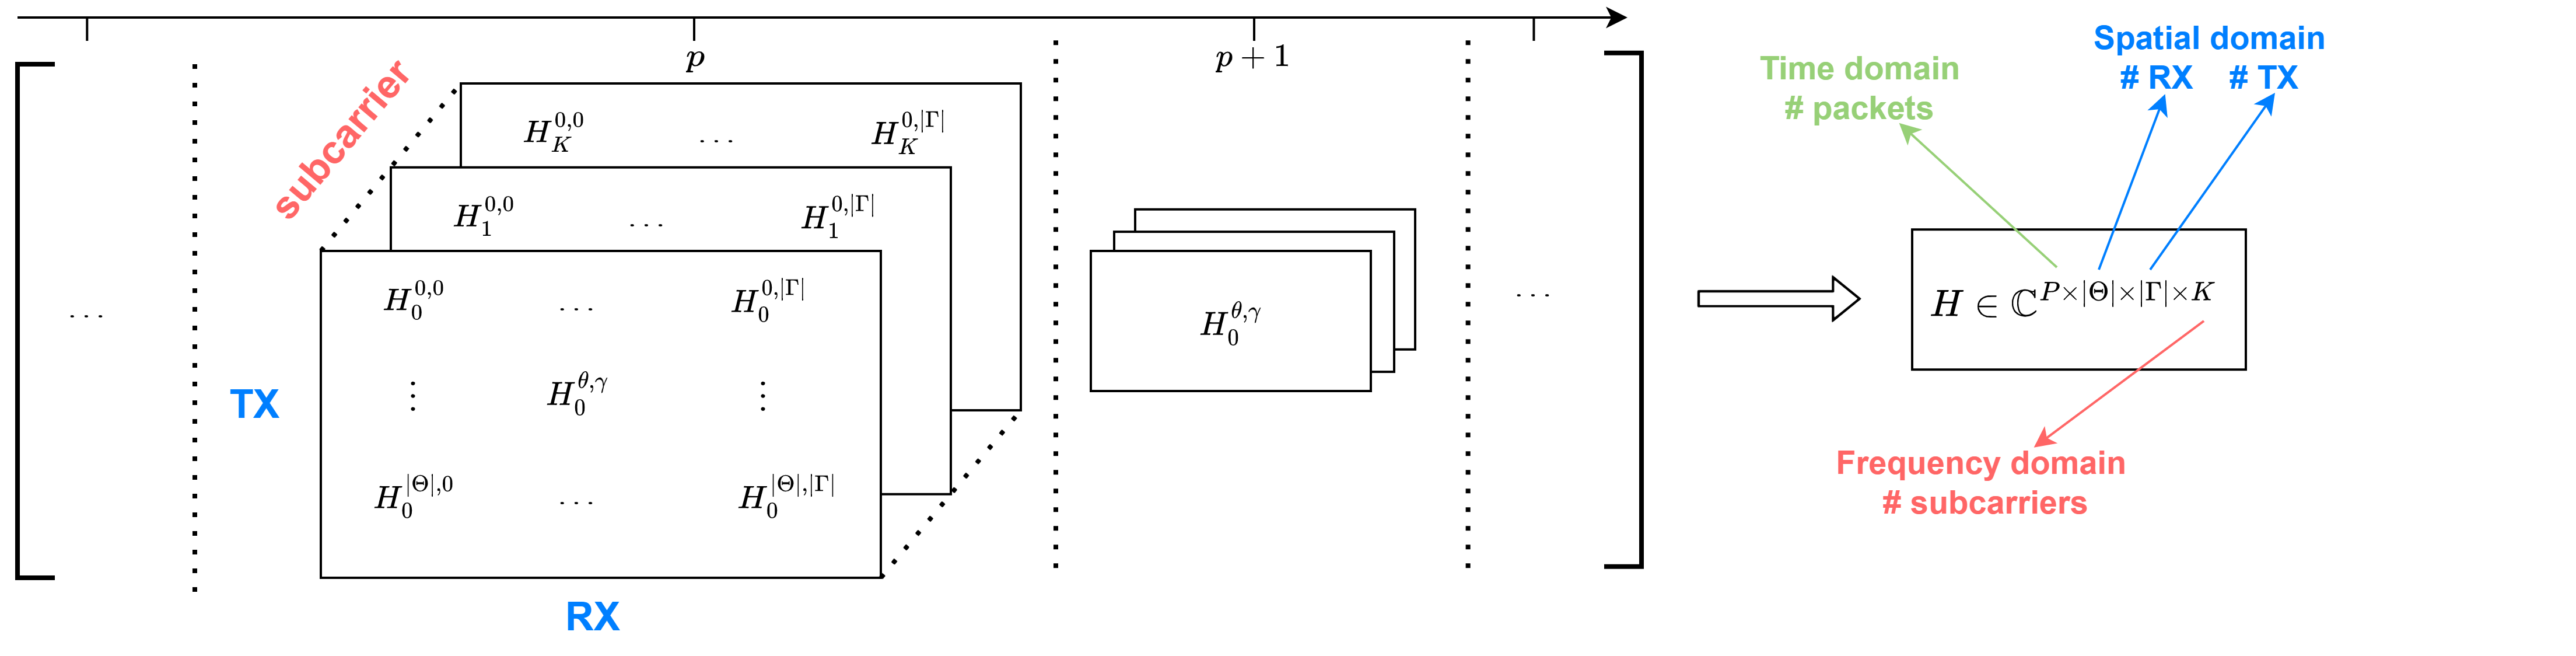
\includegraphics[width=\linewidth]{csi-matrix-2}
\caption{Representation of the CSI data as a 4D matrix.}
\label{fig:csi-4d}
\end{figure}

%\begin{equation}
%CSI = 
%\begin{bmatrix}
%H(f)^{(1,1)}_1 & H(f)^{(1,1)}_2 & \dots & H(f)^{(1,1)}_k \\
%H(f)^{(1,2)}_1 & H(f)^{(1,2)}_2 & \dots & H(f)^{(1,2)}_k \\
%\vdots & \vdots & \vdots & \vdots \\
%H(f)^{(\theta,\gamma)}_1 & H(f)^{(\theta,\gamma)}_2 & \dots & H(f)^{(\theta,\gamma)}_k \\
%\end{bmatrix}
%\end{equation}

\section{Amplitude and Phase}\label{sec:amp-pha}

As we said, from a signal using the CSI measurement we can extract two of its characteristics: amplitude and phase shift, depicted in Figure \ref{fig:amp-phase}. The amplitude represents the measurement of the maximum extent of the wave from its equilibrium position. Instead, the phase shift express the relative displacement among the same frequency radio signals measured in degrees or radians.

\begin{figure}[h!]
\centering
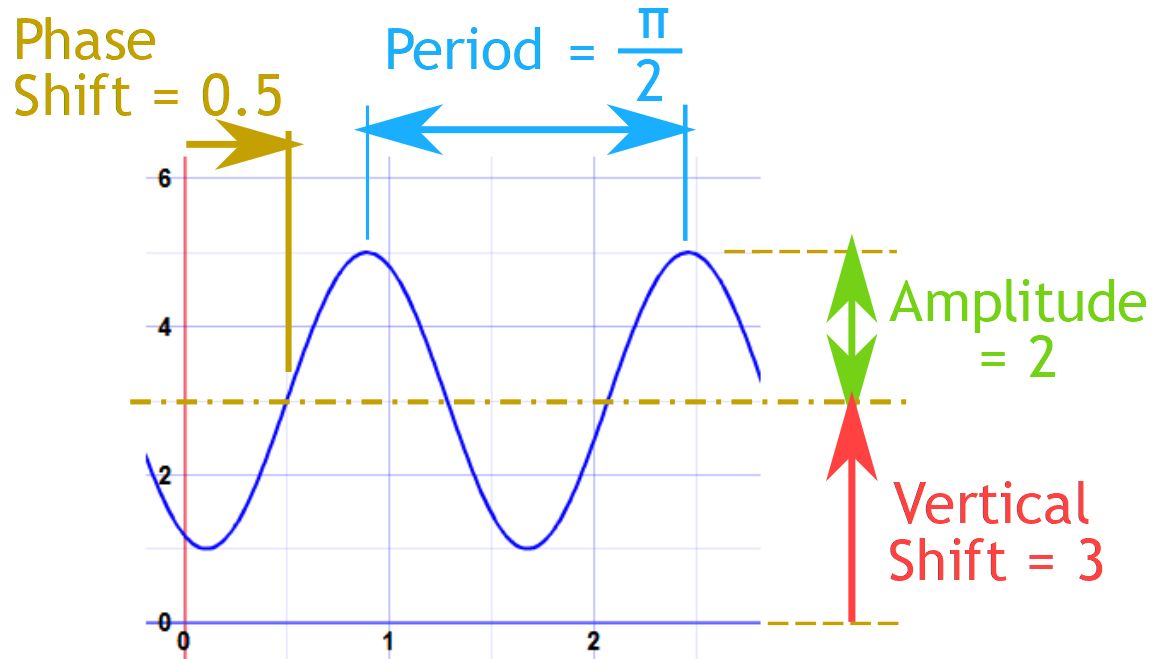
\includegraphics[width=.5\linewidth]{amplitude-phase}
\caption{Visualization of amplitude and phase of a sinusoidal signal.}
\label{fig:amp-phase}
\end{figure}

Both amplitude and phase can be easily retrieved from the CSI matrix, but they both require a step of sanitization before being used for Wi-Fi sensing based applications.

For the amplitude, the sanitization involves primarily to remove outliers added by a noisy communication channel. Outliers removal is generally performed through a sliding window mechanism on all the data sequence. In particular, for signal processing a popular choice is the Hampel filter \cite{hampel}, which define points that falls out of the closed interval $[\mu - \gamma \sigma, \mu + \gamma \sigma]$ as outliers, where $\mu$ is the median and $\sigma$ is the Median Absolute Deviation (MAD) of the sequence \cite{pads}. Instead, $\gamma$ is a parameter to control how much the outlier identification has to be strict, usually $\gamma = 3$. In other words, the Hampel filter consider as outlier any point resulting in more than $\gamma$ local MAD away from the local median inside the analyzed window.
Formally, given the amplitude of the signal for a packet $p \in P$ acquired throughout the CSI measurement, the local median is defined as follows:

\begin{equation}
\mu(\Omega^{p, k}) = \Omega^{p, k}_{\lceil w / 2\rceil},
\end{equation}
where $\Omega^{p, k}$ is defined as the set of $w$ neighboring amplitude values $a = |H(f)_k|$ of the $k$-th subcarrier, formally:

\begin{equation}
\Omega^{p, k} = \{ a^{p - \lfloor w / 2 \rfloor}, \dots, a^{p + \lfloor w / 2 \rfloor} : a^{p - \lfloor w / 2 \rfloor} < a^{p + \lfloor w / 2 \rfloor} \}.
\end{equation}

Therefore, the local MAD can be defined as follows:

\begin{equation}
\sigma(\Omega^{p, k}) = \mu \left( | \Omega^{p, k}_i - \mu ( \Omega^{p, k} ) | \right), \forall i, s.t. \: 1 \le i \le w.
\label{eq:local-mad}
\end{equation}

In the end, we have that each point outside the following interval is considered an outlier:

\begin{equation}
limit^{p, k} = \mu(\Omega^{p,k} \pm \gamma * \sigma(\Omega^{p,k})).
\end{equation}

Each value defined as outlier will be then replaced with the previous non-outlier value. An example of the result of this process is shown in Figure \ref{fig:amp-san}.

\begin{figure}[h!]
\centering
\begin{subfigure}{.49\textwidth}
	\centering
	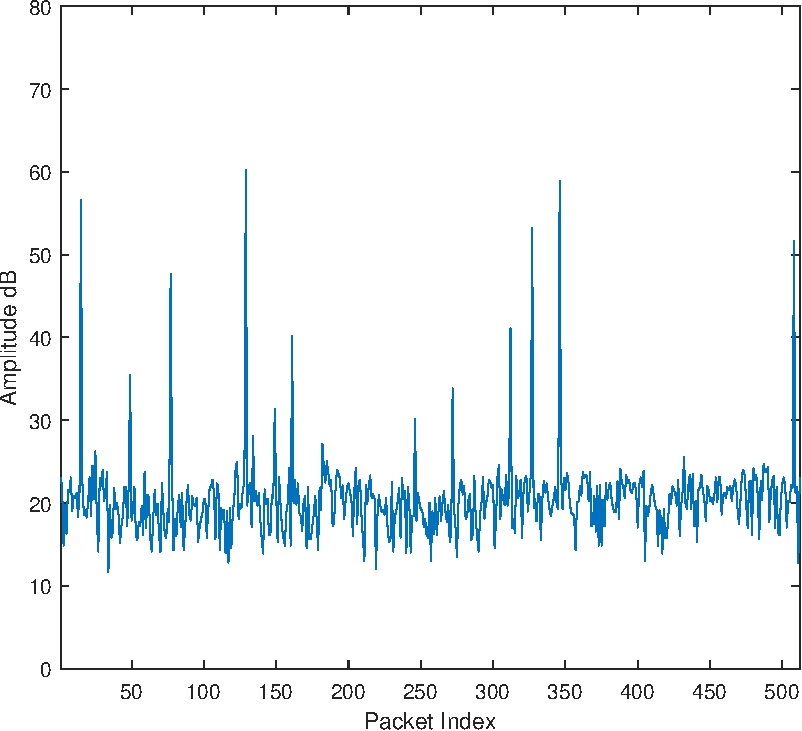
\includegraphics[width=.9\linewidth]{Amplitude TX1-RX1 vs Packet Index subcarrier_1}
	\caption{}
\end{subfigure}
\begin{subfigure}{.49\textwidth}
	\centering
	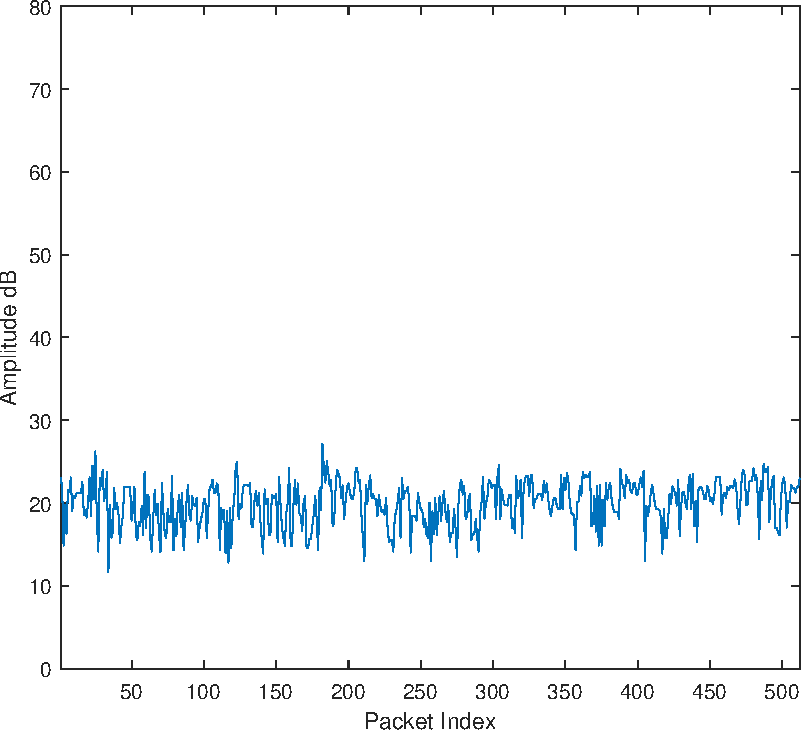
\includegraphics[width=.9\linewidth]{Amplitude TX1-RX1 vs Packet Index (Sanatized) subcarrier_1}
	\caption{}
\end{subfigure}
\caption{Result of the amplitude sanitization procedure. In (a) the raw amplitude collected for a single subcarrier and in (b) the result of the sanitiazation process for the same sample.}
\label{fig:amp-san}
\end{figure}

Regarding the phase, random noise and time not synchronized clocks make the phase almost unusable, but based on \cite{pads, spot, phasefi} is possible to mitigate such problems and produce more reliable phase information.

The raw phase collected by the CSI measurement can be expressed as follows:

\begin{equation}
\angle \hat{H}(f)_k = \angle H(f)_k + 2 \pi \frac{m_k}{N} \Delta t + \beta + Z,
\end{equation}
where $\angle H(f)_k$ is the real phase of the signal for the $k$-the subcarrier, $\Delta t$ is the timing offset at the receiver, $\beta$ is the unknown phase offset, $Z$ represents the noise of the signal, while $m_k$ and $N$ respectively correspond to the subcarrier index and the Fast Fourier Transform (FFT) size given by the standard IEEE 802.11n. Since the $\Delta t$ and $\beta$ values are unknown the real phase cannot be retrieved. However, it is possible to apply a linear transformation considering phase across the entire frequency band and therefore mitigate the effect of random noise.
The linear transformation is based on two terms:

\begin{equation}
a = \frac{\angle \hat{H}(f)_K - \angle \hat{H}(f)_1}{m_K - m_1},
\end{equation}

\begin{equation}
b = \frac{1}{K} \sum_{k=1}^K \angle \hat{H}(f)_k,
\end{equation}
where $a$ is the slope of the received response's phase and $b$ is the offset. Then, using these terms we can compute an estimate of the real phase as follows:

\begin{equation}
\angle \tilde{H}(f)_k = \angle \hat{H}(f)_k - a m_k - b.
\end{equation}

An example of the output of this sanitization step is shown in Figure \ref{fig:pha-san}.

\begin{figure}[h!]
\centering
\begin{subfigure}{.49\textwidth}
	\centering
	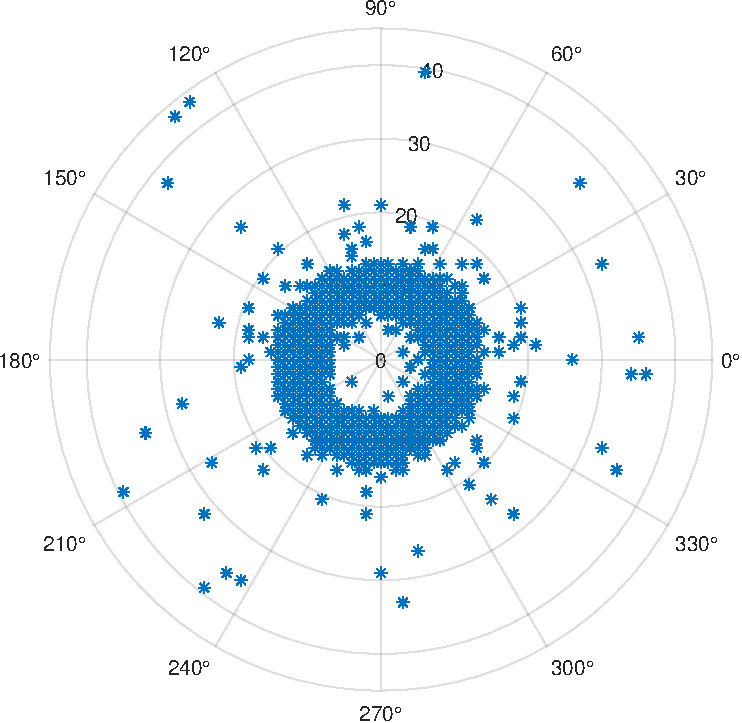
\includegraphics[width=.9\linewidth]{raw_phase subcarrier_42}
	\caption{}
\end{subfigure}
\begin{subfigure}{.49\textwidth}
	\centering
	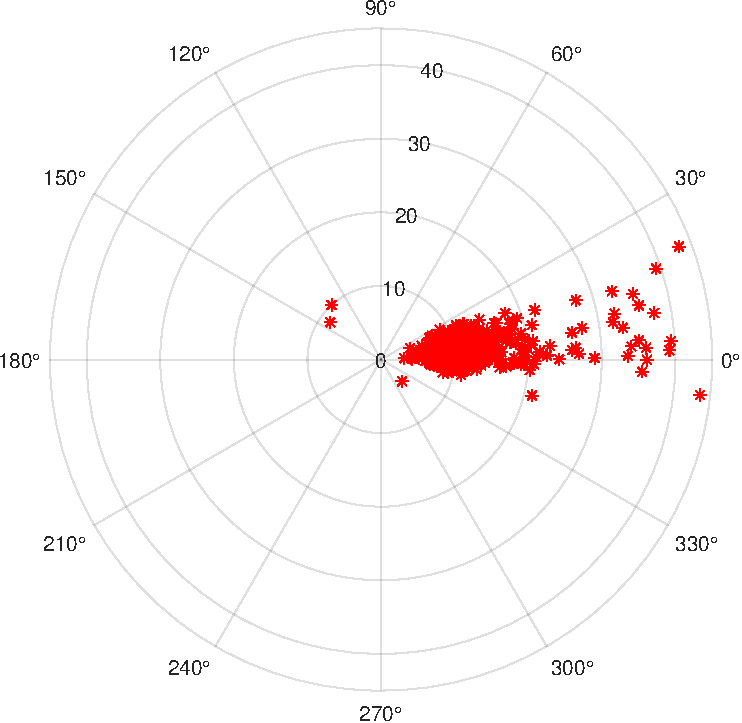
\includegraphics[width=.9\linewidth]{sanitized_phase subcarrier_42}
	\caption{}
\end{subfigure}
\caption{Result of the phase sanitization procedure. In (a) the raw phase collected for a single subcarrier and in (b) the result of the sanitiazation process for the same sample.}
\label{fig:pha-san}
\end{figure}

\chapter{Deep Learning}\label{cap:dl}

In the following chapter the Deep Learning concepts needed to understand the proposed method are illustrated. In particular, in Section \ref{sec:intro-dl} will be presented an introduction on Machine Learning and Deep Learning. Moreover, neural networks, deep neural networks and convolutional neural networks will be respectively described in Sections \ref{sec:nn}, \ref{sec:dnn} and \ref{sec:cnn}. Finally, Trasnformers will be introduced in Section \ref{sec:transformer}.

\section{Introduction}\label{sec:intro-dl}

Machine Learning (ML) is a branch of Artificial Intelligence (AI) that with respect to traditional programming methods induces a model to autonomously learn patterns from the raw input data. The model will learn patterns autonomously without any explicit encoding of the patterns to search for, during a so-called training phase, in which the parameters of the model are tuned accordingly to the provided data.
Moreover, one of the most important phase in the ML pipeline is the feature extraction phase in which the features that are more relevant to address the task are identified and extracted from the raw input data, based on statistical techniques or on the human knowledge of the task context. Then, the extracted features are fed to one of the several ML models (e.g. Decision Trees, Support Vector Machines and others) and the training phase is performed.
ML techniques have shown significant better results than other techniques, especially for complex tasks in which Deep Learning models are applied. In fact, Deep Learning (DL) is specific class of Machine Learning (ML) algorithms in which deep models are used to autonomously extract progressively higher-level features from the raw input data, as shown in Figure \ref{fig:dl-ml}.

\begin{figure}[h!]
\centering
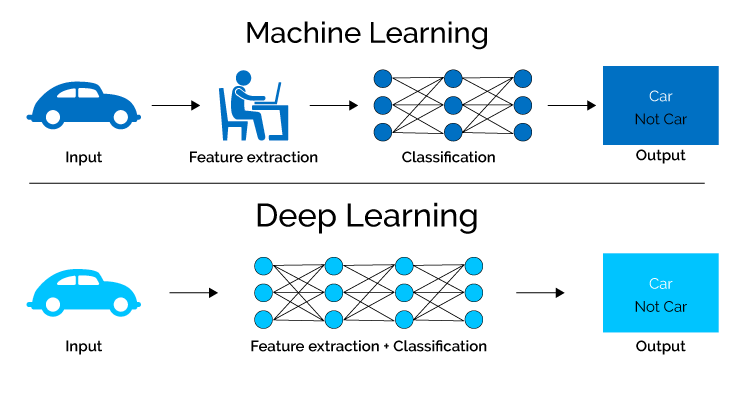
\includegraphics[width=.7\linewidth]{dl}
\caption{Representation of Machine Learning and Deep Learning pipelines.}
\label{fig:dl-ml}
\end{figure}

The training phase of a ML model can be performed in several ways based on the type of data we have:
\begin{itemize}
\item \textbf{Supervised}: is the most common case, in which input-output pairs are available to train the model. The training phase will be characterized by an optimization of the parameters to minimize the error of the model for a given input with respect to the associated output, called ground truth;
\item \textbf{Unsupervised}: we don't have any pairs but only a set of data we want to categorize based on the available features. In the training procedure we will categorize samples based on statistical approaches to detect patterns in the input or a typical distribution of the data;
\item \textbf{Semi-supervised}: only a small subset of the raw input have an associated output in the dataset and for all the other samples we have only the raw input. In this case, we want to determine the output of the samples which are not classified and produce a model able to generalize also for samples that differ from the ones of the original subset;
\item \textbf{Reinforcement}: in this case we don't have a particular set of data available at the start of the training procedure, but we will perform actions in the real world and observe the response of the environment. Then, based on the response we will be able to classify our actions as positive or negative, rewarding the model accordingly for the prediction.
\end{itemize}

\section{Neural Networks}\label{sec:nn}
Neural Networks (NNs) are one of the most popular ML models available in the field. A NN is a computational model inspired by biological neural networks present in human brains. They are composed by artificial neurons that, once received a signal from nearby neurons, will process it and output a value as input to the neurons linked to them. The signal is usually represented by real numbers, while the processing inside a neuron is performed by a non-linear function, called activation function.
Each link between neurons has a weight, which indicates how much the output of the previous neuron contributes to the output of the following one. Formally, a neuron is defined as follows:
\begin{equation}
out = \sum_{i=0}^N w_i x_i + b,
\end{equation}
where $N$ is the number of linked neurons, $w_i$ is the weight associated to the $i$-th link, $x_i$ is the signal received on the $i$-th link and $b$ is a term called bias which is used to shift the output.

Then, the activation function $f$ is applied and the final output $y$ of the neuron will be determined as:

\begin{equation}
y = f(out).
\end{equation}

The activation function can be any function but it must be differentiable since we need to compute gradients during the training phase. Several activation functions have been proposed and experimented by researchers in order to perform a more efficient training procedure and produce better results and below some of the most used functions are illustrated:
\begin{itemize}
\item \textbf{Linear function}: doesn't perform any change to $out$, simply defined as:
\begin{equation}
f(x) = x
\end{equation}
\item \textbf{Sigmoid function}: produces values in the range $[0, 1]$, defined as:
\begin{equation}
f(x) = \frac{1}{1 + e^{-x}}
\end{equation}
\item \textbf{Hyperbolic tangent function}: similar to the sigmoid function but produces values in the range $[-1, 1]$, defined as:
\begin{equation}
f(x) = \tanh x
\end{equation}
\item \textbf{Rectified Linear Unit (ReLU)}: one of the most used functions for NNs and outputs values in the range $[0, \infty)$, defined as:
\begin{equation}
f(x) = \max (0, x)
\end{equation}
\end{itemize}

In addition, as shown in Figure \ref{fig:dnn}, neurons are grouped in layers, and the first and last layer are respectively called input layer and output layer, while all the other intermediate layers, are called hidden layers.

\begin{figure}[h!]
\centering
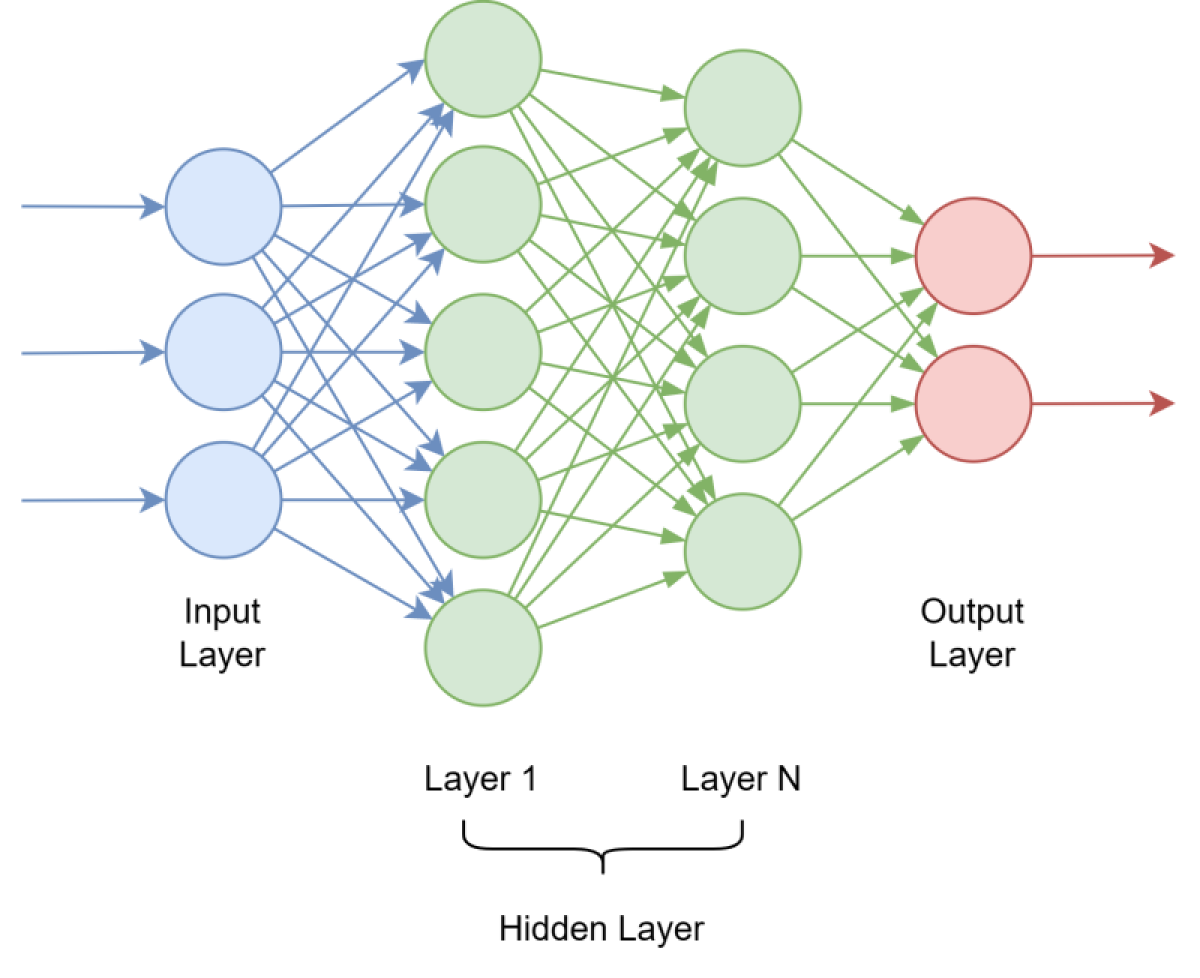
\includegraphics[width=.8\linewidth]{dnn}
\caption{Representation of a standard neural network.}
\label{fig:dnn}
\end{figure}

\subsection{Learning phase}

Given a neural network with training pairs $(x_i,y_i)$ the goal of the learning phase is to find the optimal weights $W_l$ for each layer $l$.

In order to do this we need to set up an optimization problem trying to find the weights $W$ which minimize the error produced by the model on the dataset samples:
\begin{equation}
\min_{W} \sum_i L_W(x_i, y_i).
\end{equation}

In the formula, $L_W$ is the so-called loss function which computes the \textit{distance} between the prediction of the network with weights $W$ on sample $x_i$ with respect to the ground truth $y_i$.
In some cases it is possible to address this problem finding a closed form solution which let us find the optimal parameters directly, but in the general case a non-linear optimization technique is used. The most used optimization technique for neural networks is the Gradient Descent.

The Gradient Descent (GD) is a first-order iterative minimization algorithm. It starts from an initial guess of the optimal weights $W^0$ and computes the loss value on that point for a sample, i.e. $L_W^0(x_i, y_i)$. Then, computing the gradient for that point, $\nabla L_{W^0}(x_i, y_i)$, we know the direction of the steepest increase of the loss function, but since we want to minimize the function we move the new guess of the optimum based on the value given by minus the gradient. Then, we repeat from the start and we continue moving until reaching the minimum value of the loss function.

Formally, we move based on the so-called gradient descent rule:

\begin{equation}
W^t \leftarrow W^{t-1} - \alpha \nabla L_{W^{t-1}}(x_i, y_i),
\end{equation}

where $\alpha$ is the learning rate which modulates the length of the step to take at each update.

In order to compute the new weights for each layer $l$ a computational technique called backpropagation is used since we need to update each weight based on how much it influences the final error. The backpropagation is able to compute efficiently the gradients with respect to each individual weight using the chain rule and iterating backward from the last layer to the first one by reducing the number of redundant computations.
%In fact, carrying over the dimension of the output which is 1 the matrix multiplications performed in order to compute the gradients are less than in a regular forward computation of the gradients.

\subsection{Loss function}
The loss function is one of the components that impacts more the results of a neural network since the weights are determined by the gradients of it. There are several loss functions that are commonly used in the state of the art for neural networks and in the following the most used ones are reported:
\begin{enumerate}
\item \textbf{Mean Squared Error (MSE)}: given $\hat{y}$ as the vector of $n$ predictions and $y$ as the ground truth values associated to the predictions, the MSE is defined as:
\begin{equation}
MSE = \frac{1}{n} \sum_{i=1}^n (y_i - \hat{y}_i)^2.
\end{equation}
\item \textbf{Binary Cross-Entropy (BCE)}: loss used for classification tasks in which we have only 2 classes, defined as follows:
\begin{equation}
BCE = - \frac{1}{n} \sum_{i=1}^n y_i \log (\hat{y}_i) + (1 - y_i) \log (1 - \hat{y}_i).
\end{equation}
\item \textbf{Categorical Cross-Entropy (CCE)}: used when we have more than 2 classes and each label is represented as one-hot encoding. Given $\hat{y}_i$ and $y_i$ as one hot encoding vectors, and $C$ classes, we can define the loss as follows:
\begin{equation}
CCE = - \frac{1}{n} \sum_{c=1}^C y_{i, c} \log (\hat{y}_{i, c}).
\end{equation}
\end{enumerate}

\section{Deep Neural Networks}\label{sec:dnn}

Deep Neural Networks (DNNs) are an extension of simple neural networks, in fact a DNN is characterized by several hidden layers which are used to extract features that are progressively higher-level. In general, DNNs have an higher power of representation and abstraction with respect to NNs, which allow them to perform incredibly better for more complex and demanding tasks.
A consequence of the higher number of layers of DNNs is the increase of the number of parameters of the model. So, in general the training procedure for DNNs is more computationally intensive and longer than standard neural networks since the higher number of parameters and bigger datasets rise a whole new set of problems that are not present in neural networks, for example the vanishing gradients problem.

\section{Convolutional Neural Networks}\label{sec:cnn}

A Convolutional Neural Network (CNN) is a particular type of neural network especially suited for computer vision tasks. A CNN is based on the convolution operator, which is defined in the continuous space as follows:
\begin{equation}
(f \star g)(x) = \int_{-\pi}^{\pi} f(t) g(x-t) dt,
\label{eq:conv}
\end{equation}
where $f$ and $g$ are two real functions defined in the interval $[-\pi, \pi]$ and $\star$ represents the convolution operator.
In Eq. \ref{eq:conv} the function $g(x-t)$ is called kernel, or convolutional kernel, instead the result of the convolution is usually called feature map in the deep learning field.

The convolution has several useful properties that determined the success of CNNs, in particular the convolution is shift-equivariant. Formally, we can define the shift-equivariant property as follows:
\begin{equation}
f(x - x_0) \star f(x) = (f \star g)(x-x_0),
\end{equation}
which means that applying a translation $x_0$ before the convolution or after produces the same result. This can be extremely useful for the processing of images, for example for the task of object detection if we can recognize an object in a particular location of the images using a CNN we are able to recognize it also in any other position thanks to the shift-equivariant property of the convolution.
In the discrete case the convolution can be redefined in the following way:
\begin{equation}
(f \star g)[x] = \sum_{i=-\infty}^{\infty} f[i]g[x-i].
\end{equation}

Moreover, the convolution can also be defined for any other dimension. For 2D domains, like RGB images, for each channel we define the convolution as follows:
\begin{equation}
(f \star g)[x, y] = \sum_i \sum_j f[i, j] g[x-i, y-j],
\end{equation}
and for 3D domains, like voxels, as:
\begin{equation}
(f \star g)[x, y, z] = \sum_i \sum_j \sum_k f[i, j, k] g[x-i, y-j, z-k],
\end{equation}

In CNNs the learned parameters are the kernel weights that are going to be tuned during the training phase in order to extract significant features of the input data. 

CNNs are particular useful for tasks related to images but in general images are a type of data that can be very high dimensional resulting in a slower training with respect to other type of data. So, in order to reduce the size of the images and by consequence make the training faster, pooling layers are used.

One of the most popular type of pooling layer is max-pooling. Max-pooling is applied to the whole image like convolution using a sliding window, defining its size and the stride that it will perform at each step. Then, each window is reduced to a single value simply by taking the maximum, and by consequence producing a lower dimensional image.

Therefore, a CNN architecture is composed by several layers of convolutions and pooling. Moreover, depending on the task, a fully connected layer can be positioned at the end of the network to process the features extracted in the previous layers and produce a final classification. An example of a CNN architecture can be seen in Figure \ref{fig:cnn}.

\begin{figure}[h!]
\centering
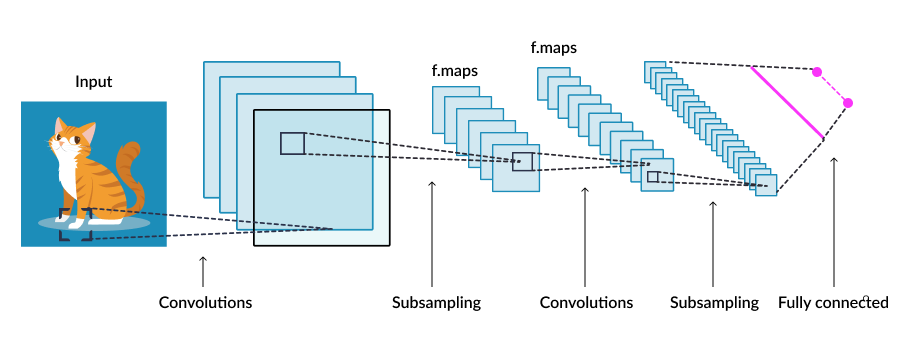
\includegraphics[width=\linewidth]{cnn}
\caption{Architecture of a Convolutional Neural Network.}
\label{fig:cnn}
\end{figure}

Regarding other key properties of CNNs, it is very important also the weight-sharing. In fact, we apply the same kernel weights to each dimension of the input, sliding the kernel on the image. Instead, in a standard NN we have a different weight for each dimension of the input. This allows CNNs to be composed of less parameters and therefore be less computational demanding, but more importantly we have that the same pattern present in different locations in an image can be extracted multiple times efficiently by the same filter.

\section{Transformers}\label{sec:transformer}

One of the architectures which has gained a lot of popularity in the state of the art lately are transformers. They showed extremely good performances for Natural Language Processing (NLP) tasks but also for tasks with different input data like images \cite{vit}.
A transformer has an encoder-decoder architecture, shown in Figure \ref{fig:transformer}, and it is characterized by the use of a so-called attention mechanism \cite{attention-is-all-you-need}. 

\begin{figure}[h!]
\centering
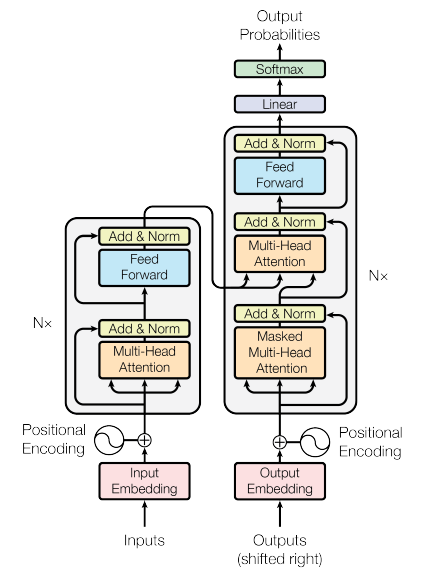
\includegraphics[width=.6\linewidth]{transformer}
\caption{Architecture of a transformer.}
\label{fig:transformer}
\end{figure}

The attention mechanism is employed inside the Multi-Head Attention layers, shown in Figure \ref{fig:mha}, which are present both in the encoder and in the decoder. A Multi-Head Attention layer takes three vectors in input, called respectively queries $Q$, keys $K$ and values $V$. Moreover, queries $Q$ and keys $K$ have both size $d_k$, and values $V$ has size $d_v$.

The attention mechanism inside a Multi-Head Attention layer is performed by a so called Scaled Dot-Product Attention block. This block is going to compute the dot products between $Q$ and $K$, divide the result by $\sqrt{d_k}$ and apply the softmax function to obtain a set of weights on the values $V$. Formally, in matrix form we have:
\begin{equation}
\text{Attention}(Q, K, V) = \text{softmax} \left( \frac{QK^T}{\sqrt{d_k}} \right) V.
\end{equation}

\begin{figure}[h!]
\centering
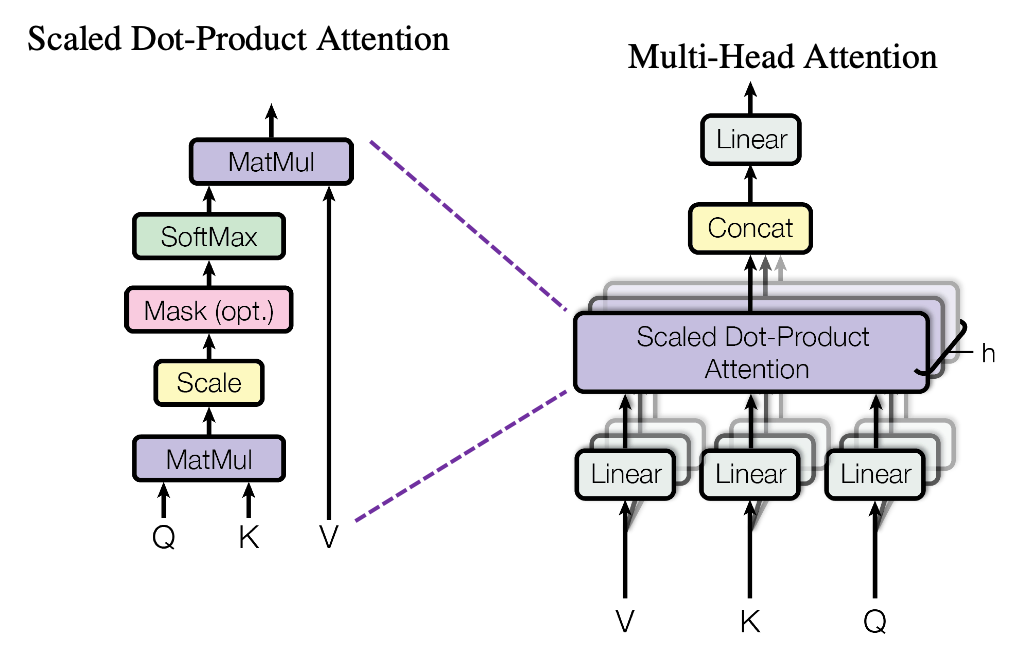
\includegraphics[width=.7\linewidth]{multi-head-attention}
\caption{Graphical representation of a Multi-Head Attention layer.}
\label{fig:mha}
\end{figure}

Instead of performing a single attention function, before applying the Scaled Dot-Product Attention, the three vectors queries, keys and values are linearly projected $h$ times and the attention is computed in parallel yielding $h$ output vectors. Then, the outputs are concatenated and once again projected producing the final output of the Multi-Head Attention layer. Formally, we have the following:

\begin{gather}
\text{MultiHead}(Q, K, V) = [A_1, A_2, \dots, A_h] W^O, \\
A_i = \text{Attention}(QW_i^Q, KW_i^K, VW_i^V) \quad \text{ where } 0 \le i \le h,
\end{gather}

where $W_i^Q, W_i^K, W_i^V$ are the projection parameters respectively for the queries, keys and values, and $W^O$ is the projection parameters for the output.

In a transformer, as we can see from its architecture, we have three Multi-Head Attention layers. The first in the encoder is used to learn relationships among all the tokens in any position in the input sequence. In this case, queries, keys and values comes all from the same place, i.e. the output of the previous layer in the encoder. In this case the attention mechanism is referred to as self-attention. Instead, the second and third Multi-Head Attention layers are in the decoder. The first of them acts similarly to the one in the encoder performing the attention mechanism on the output of the previous layer. Instead, the second and last layer of Multi-Head Attention is different from the previous two, in fact the queries come from the previous decoder layer, and the keys and values come from the output of the encoder.

Finally, another concept about transformers that is relevant to their functioning is positional encoding. In fact, this concept allows transformers to be aware of the order of the sequence, injecting some information about the relative or absolute position of the tokens in the sequence. In practice, positional encoding vectors are added to the input embeddings of the encoder and decoder. In the original paper of transformers the following positional encoding vectors are used:
\begin{equation}
\begin{split}
PE(pos, 2i) = &\sin \left( \frac{pos}{10000^{2i / d_{model}}} \right), \\
PE(pos, 2i+1) = &\cos\left( \frac{pos}{10000^{2i / d_{model}}} \right).
\end{split}
\end{equation}
Moreover, transformers are not only composed by attention layers, in fact they also rely on standard feed forward neural networks, skip connections and normalization layers, following Figure \ref{fig:transformer}.


\chapter{Method}\label{cap:method}
In this chapter the method applied in this work will be presented and the design choices motivated. In particular, the estimation and sanitization of the CSI data will be illustrated respectively in Sections \ref{sec:csi-est} and \ref{sec:csi-san}. Finally, the deep learning architecture of the proposed method will described in details in Section \ref{sec:arch}.

\section{CSI estimation}\label{sec:csi-est}

The estimation of the Channel State Information (CSI) was performed considering only a single transmitting and a single receiving antenna. As presented in Section \ref{sec:csi}, given $\Theta = 1$ and $\Gamma = 1$ representing respectively the number of transmit and receive antennas, and $K = 50$ as the number of OFDM subcarriers, we can model the channel frequency response as follows:
\begin{equation}
y = H(f) x + \omega,
\end{equation}
where $y$ is the received signal, $x$ is the transmitted signal, $\omega$ is the noise factor and $H(f)$ is the channel frequency response.

Now, considering each subcarrier $k$ we can obtain the frequency response $H(f)_k^{\theta, \gamma}$ for each $\theta \in \Theta$ and $\gamma \in \Gamma$ antennas. However, in our case the number of both transmitting and receiving antennas is fixed to 1, so we simply obtain $H(f)_k$ which is a vector of $K$ complex values. Finally, amplitude and phase of $H(f)_k$ are defined as described in Eq. \ref{eq:h(f)}.

Considering the collected amplitude and phase values we have two matrices of size $P \times K$ where $P$ is the number of packets collected and $K$ the number of subcarriers, which is equal to 50 as stated before. We can interpret these matrices as a $P \times K$ CSI image with two channels. An example of the CSI image containing both amplitude and phase can be seen in Figure \ref{fig:amp-phase-image}.

\begin{figure}[h!]
\centering
\begin{subfigure}{.49\textwidth}
	\centering
	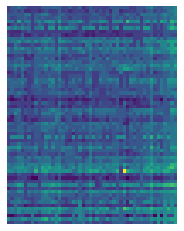
\includegraphics[width=.6\linewidth]{results/amplitude-1}
	\caption{Amplitude}
\end{subfigure}
\begin{subfigure}{.49\textwidth}
	\centering
	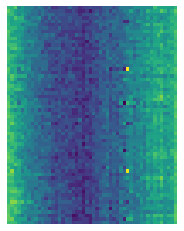
\includegraphics[width=.6\linewidth]{results/phase-1}
	\caption{Phase}
\end{subfigure}
\caption{Example of a CSI image composed by two channels with the amplitude as first one (a) and the phase as the second one (b).}
\label{fig:amp-phase-image}
\end{figure}

\section{CSI sanitization}\label{sec:csi-san}

Before using the collected CSI data a sanitization step is necessary for both amplitude and phase. The procedure described in Section \ref{sec:amp-pha} was used in order to remove the possible outliers in the amplitude and reduce the noise in the phase component. In detail, the outliers are identified computing the local median values over a fixed length sliding window. Therefore, all the values three local MAD away from the local median are considered outliers and replaced with the previous non-outlier value.
Formally, each value outside of the following interval is considered outlier:
\begin{equation}
limit^{p, k} = \mu(\Omega^{p,k} \pm 3 * \sigma(\Omega^{p,k})),
\end{equation}
where $\Omega^{p, k}$ is the set of neighboring amplitude values in the defined window size for the $p$-th packet and $k$-th subcarrier and $\sigma(\Omega^{p,k})$ is the local MAD of the specified window, defined in Eq. \ref{eq:local-mad}.

Instead, regarding the sanitization of the phase component of the CSI data acquired, a linear transformation was performed based on \cite{pads, spot, phasefi}. Formally, for each subcarrier $1 \le k \le 50$ the following transformation was applied:
\begin{equation}
\angle \tilde{H}(f)_k = \angle \hat{H}(f)_k - a m_k - b,
\end{equation}
where $\angle \hat{H}(f)_k$ is the raw phase acquired, $m_k$ is the index of the $k$-th subcarrier and the two values, $a$ and $b$, are defined as follows:
\begin{equation}
a = \frac{\angle \hat{H}(f)_{50} - \angle \hat{H}(f)_1}{m_{50} - m_1},
\end{equation}

\begin{equation}
b = \frac{1}{50} \sum_{k=1}^{50} \angle \hat{H}(f)_k.
\end{equation}

\section{Architecture}\label{sec:arch}

The architecture proposed by this work to address 3D indoor environment reconstruction from Wi-Fi data is based on the original transformer architecture and it is composed by three modules: a 2D transformer encoder, a 3D transformer decoder and a 3D CNN upscaler. The complete architecture can be seen in Figure \ref{fig:arch}. 

\begin{figure}[h!]
\centering
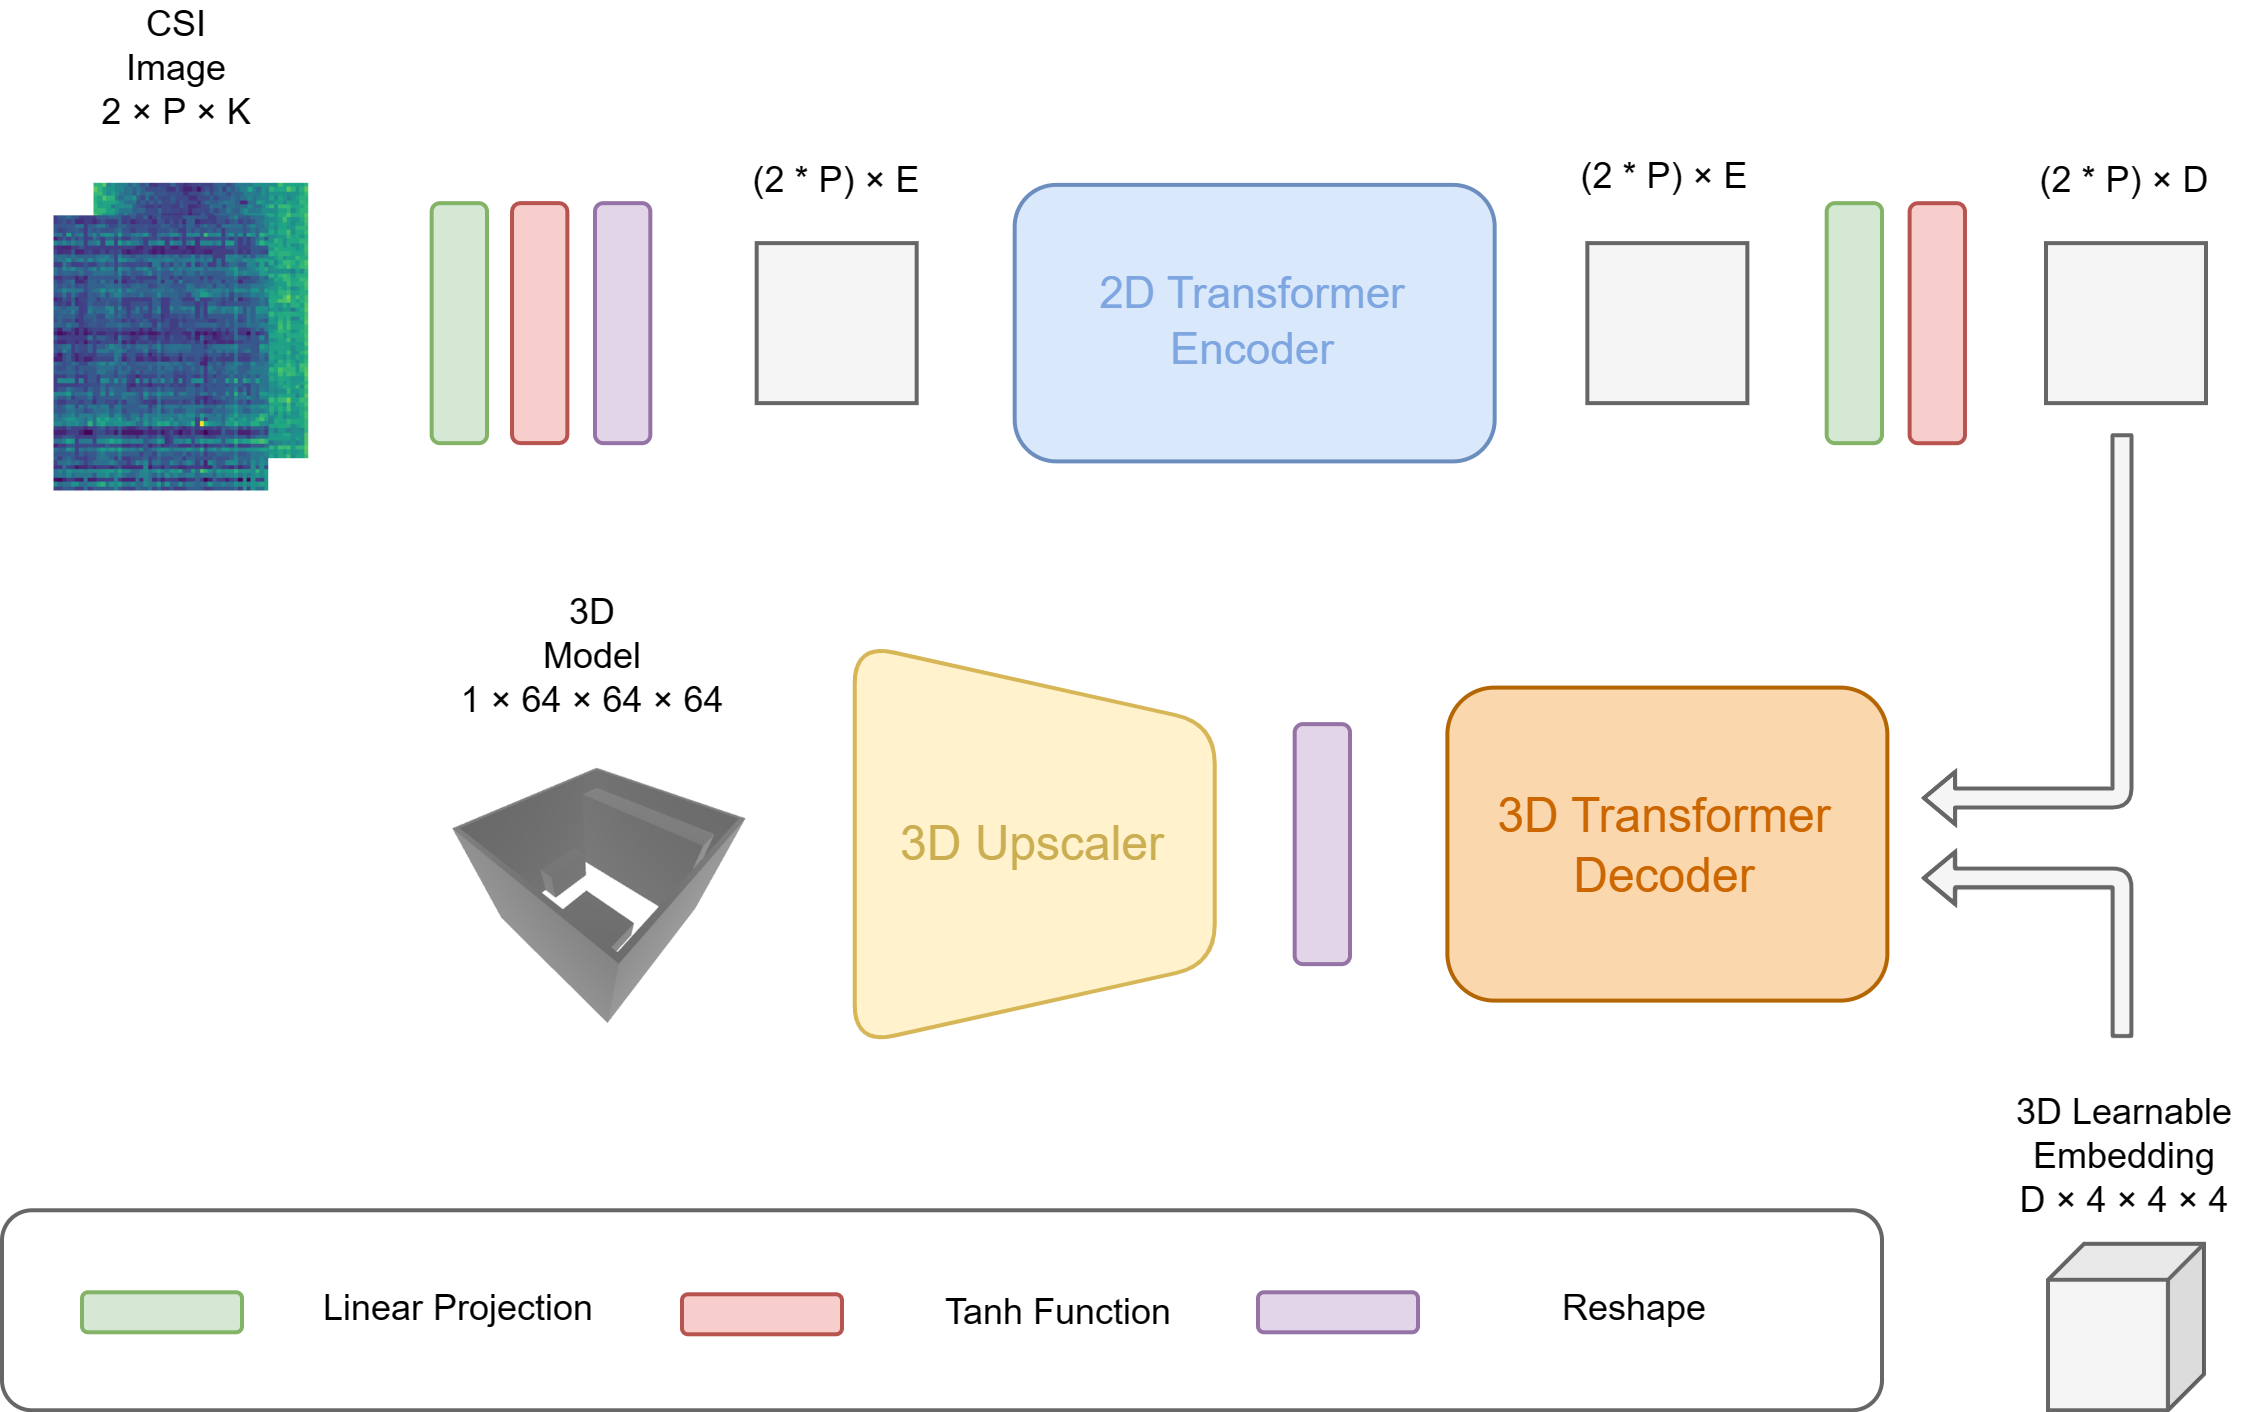
\includegraphics[width=\linewidth]{arch}
\caption{Architecture of the proposed method.}
\label{fig:arch}
\end{figure}

At high level, the 2D transformer encoder will take as input a linearly projected CSI image encoding both amplitude and phase. Instead, the 3D transformer decoder is used to obtain voxels features by cross-attending to the CSI features extracted by the encoder. Finally, the 3D CNN upscaler will upscale the voxels features in order to obtain the final complete output of the model in the target voxel space.
The CSI image $x_i \in \mathbb{R}^{2 \times P \times K}$ fed to the model is composed by two channels, the first one containing the amplitude values and the second one the phase values. Each channel has size $P \times K$, with $P = 64$ as the number of packets and $K = 50$ as the number of subcarriers. Instead, the output is composed by a voxel grid of size $64 \times 64 \times 64$ denoted as $Y \in [0,1]^{64 \times 64 \times 64}$, where any value lower than 0.5 indicates an empty voxel and an occupied one otherwise.


\subsection{2D Transformer Encoder}

The CSI image before being fed to the encoder is projected and reshaped. For each packet of both amplitude and phase a linear projection is performed which encodes the values in vectors of size $E$. Then, an hyperbolic tangent function is applied in order to scale the values in the range $[-1,1]$ and the resulting matrix is reshaped into a tensor of size $(2 * P) \times E$. The linear projection allows the model to produce embeddings enriching the information contained in the CSI, while the reshaping let the model perform the attention mechanism on a sequence composed by $2 * P$ tokens each one of size $E$.

The transformer encoder used by this work follows the same architecture of the original paper \cite{attention-is-all-you-need}, presented in Section \ref{sec:transformer}. In Figure \ref{fig:t-enc} a representation of the 2D transformer encoder is shown. The only major difference with the original transformer architecture is the absence of the positional encoding in the input of the encoder which didn't produce any relevant result to motivate its use. As shown in the figure, each transformer encoder layer is composed by $H$ multi-head attention layers, a small feed forward neural network and two normalization layers.

The 2D Transformer Encoder is characterized by two hyper-parameters: number of heads $H$ and number of layers $L_e$. Several heads $H$ for each transformer encoder layer allow the encoder to focus on different patterns with each head. Instead, the number of layers $L_e$ increases the expressiveness of the model and allows to perform attention to higher-level features.

After going through the encoder, the features extracted will be projected into a $D$-dimensional space, in the same way as described previously for the input of the encoder. Therefore, another linear projection layer with a subsequent hyperbolic target function is applied, processing the features one last time before going through the 3D transformer decoder and producing an output of size $(2 * P) \times D$.

\begin{figure}[h!]
\centering
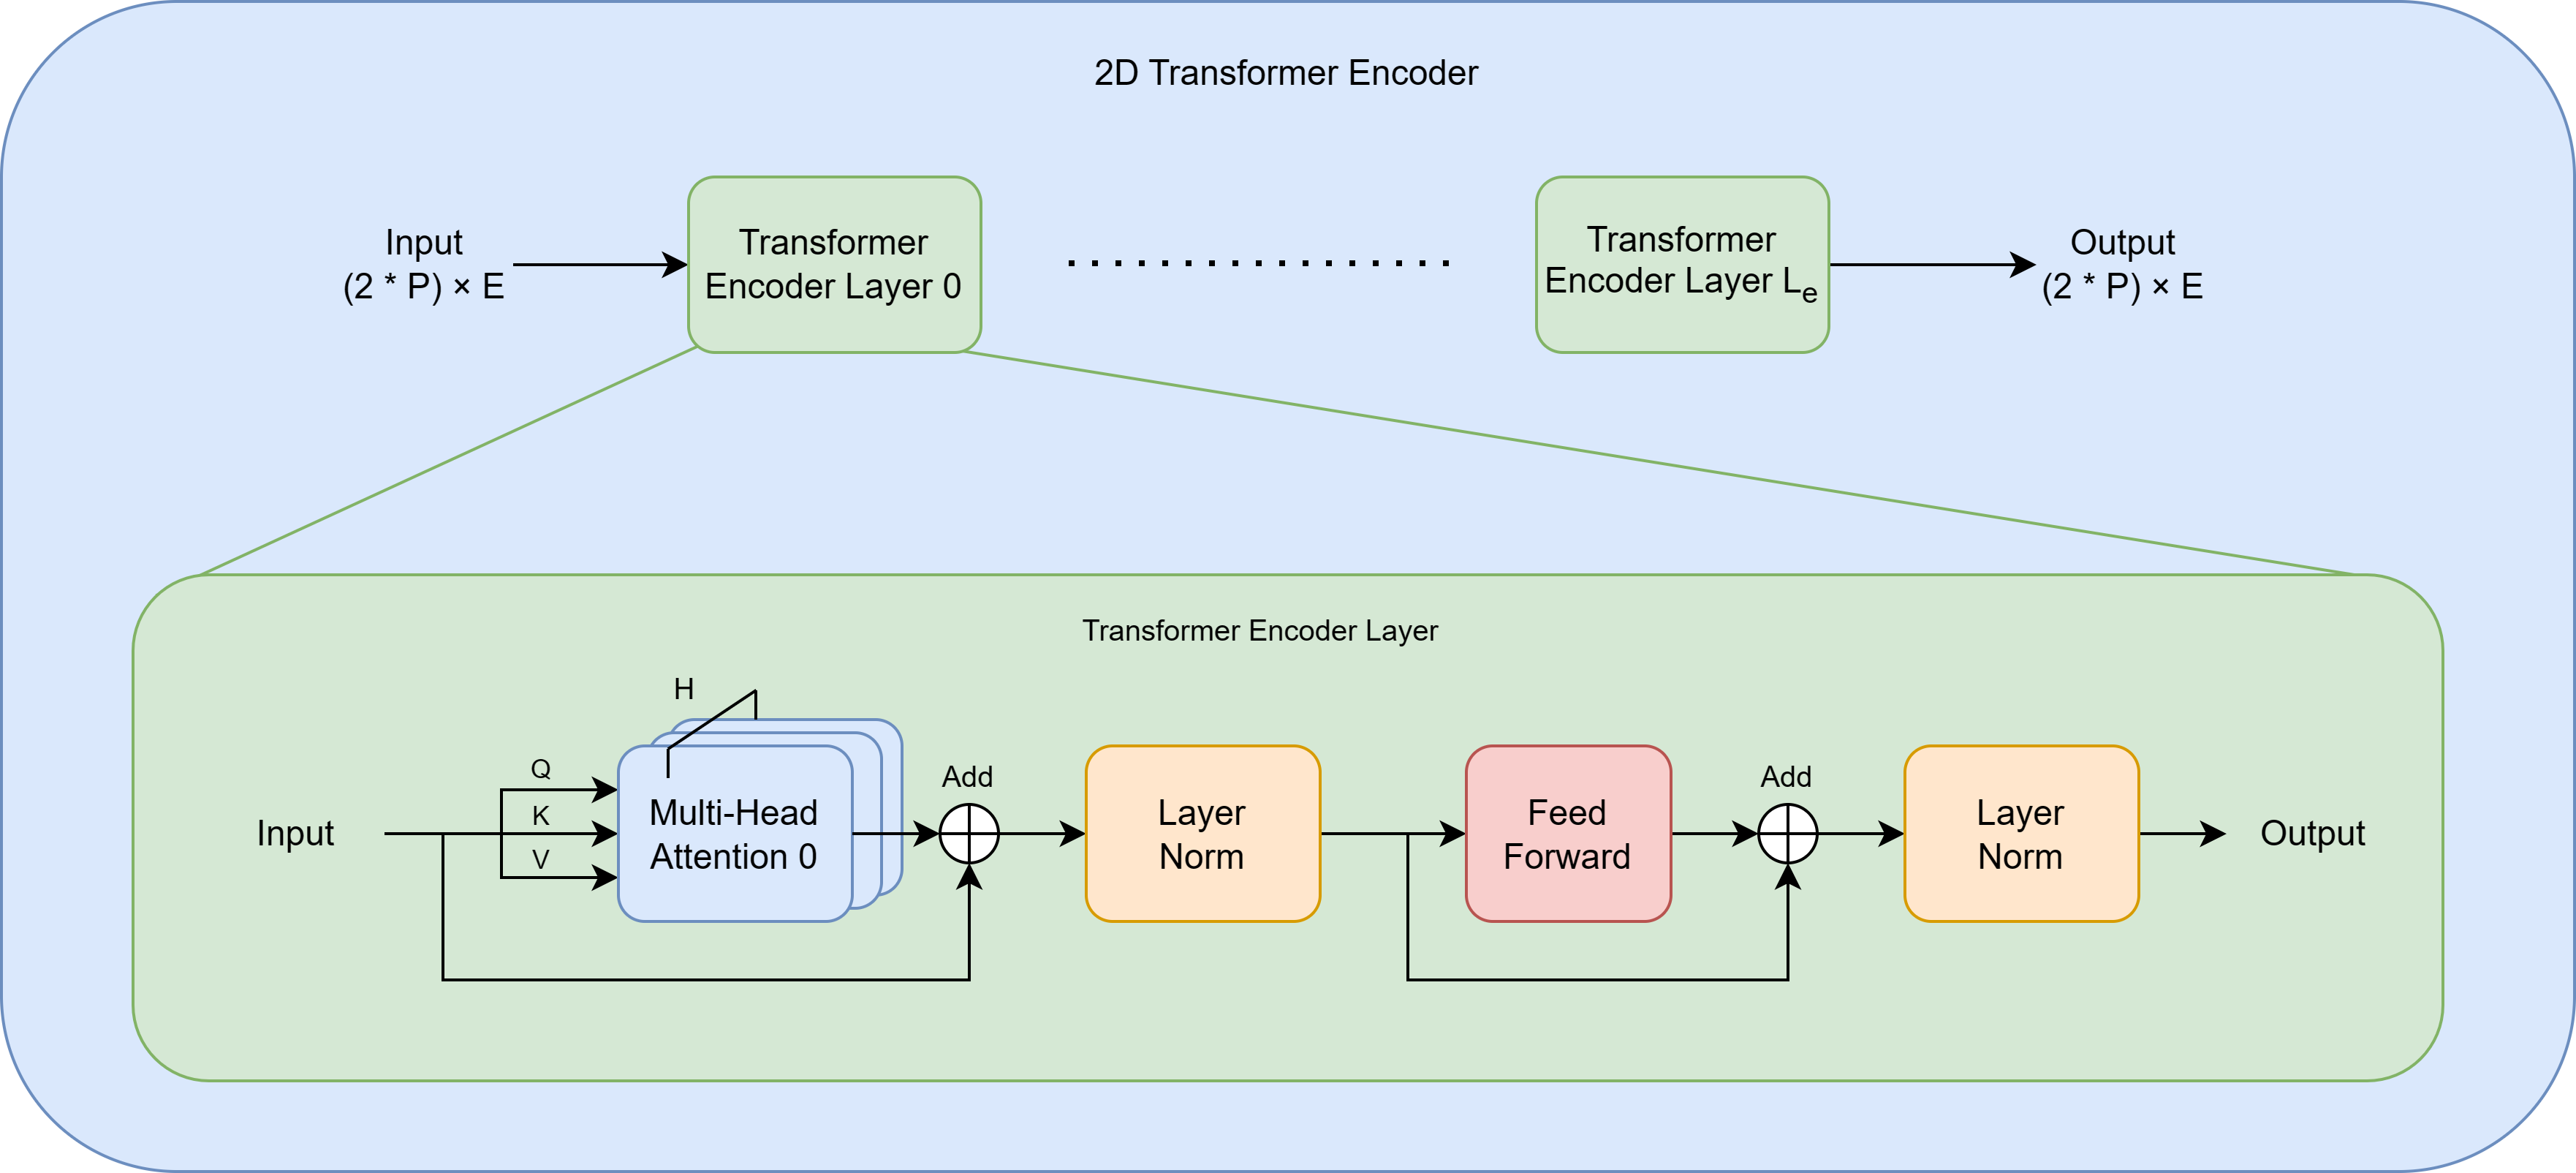
\includegraphics[width=\linewidth]{2d-trans-encoder}
\caption{Architecture of the 2D transformer encoder module.}
\label{fig:t-enc}
\end{figure}

\subsection{3D Transformer Decoder}

In the typical transformer architecture, presented in Section \ref{sec:transformer}, the decoder takes as input the result produced by the encoder which is cross-attended with the tokens previously produced by the decoder itself. However, in this case the output of the model is not a sequence and another method to substitute the original input of the decoder is used. In fact, inspired by other papers that use transformers in order to generate voxel grids, like \cite{3d-retr}, the decoder works in parallel, by taking as input learnable embeddings rather than following an autoregressive approach as in the original transformer.
These embeddings are randomly sampled from a normal distributon at the start of the training and then updated based on the loss, as normal parameters of the model.

Therefore, the input of the decoder, in addition to the output of the encoder, is composed by learnable embeddings of size $4^3 \times D$. 
The size of the learnable embeddings is based on the fact that the transformer decoder needs a sequence of tokens in which each token has size $D$, which is the same dimension of the linear projection applied to the encoder output. Instead, the length of the sequence, which is $4^3$, is assigned in this way in order to obtain a 3D space of size $4 \times 4 \times 4$ as the output of the decoder and then upscale it using the next module.

Finally, the decoder is referred to as 3D transformer decoder even if it works on a sequence of tokens since the input sequence is actually composed by flattened 3-dimensional data.

\subsection{3D Upscaler}

The last module is the 3D upscaler which is in charge of the reconstruction of the final $64 \times 64 \times 64$ output space. In Figure \ref{fig:upscaler} the architecture of the 3D upscaler is shown.

\begin{figure}[h!]
\centering
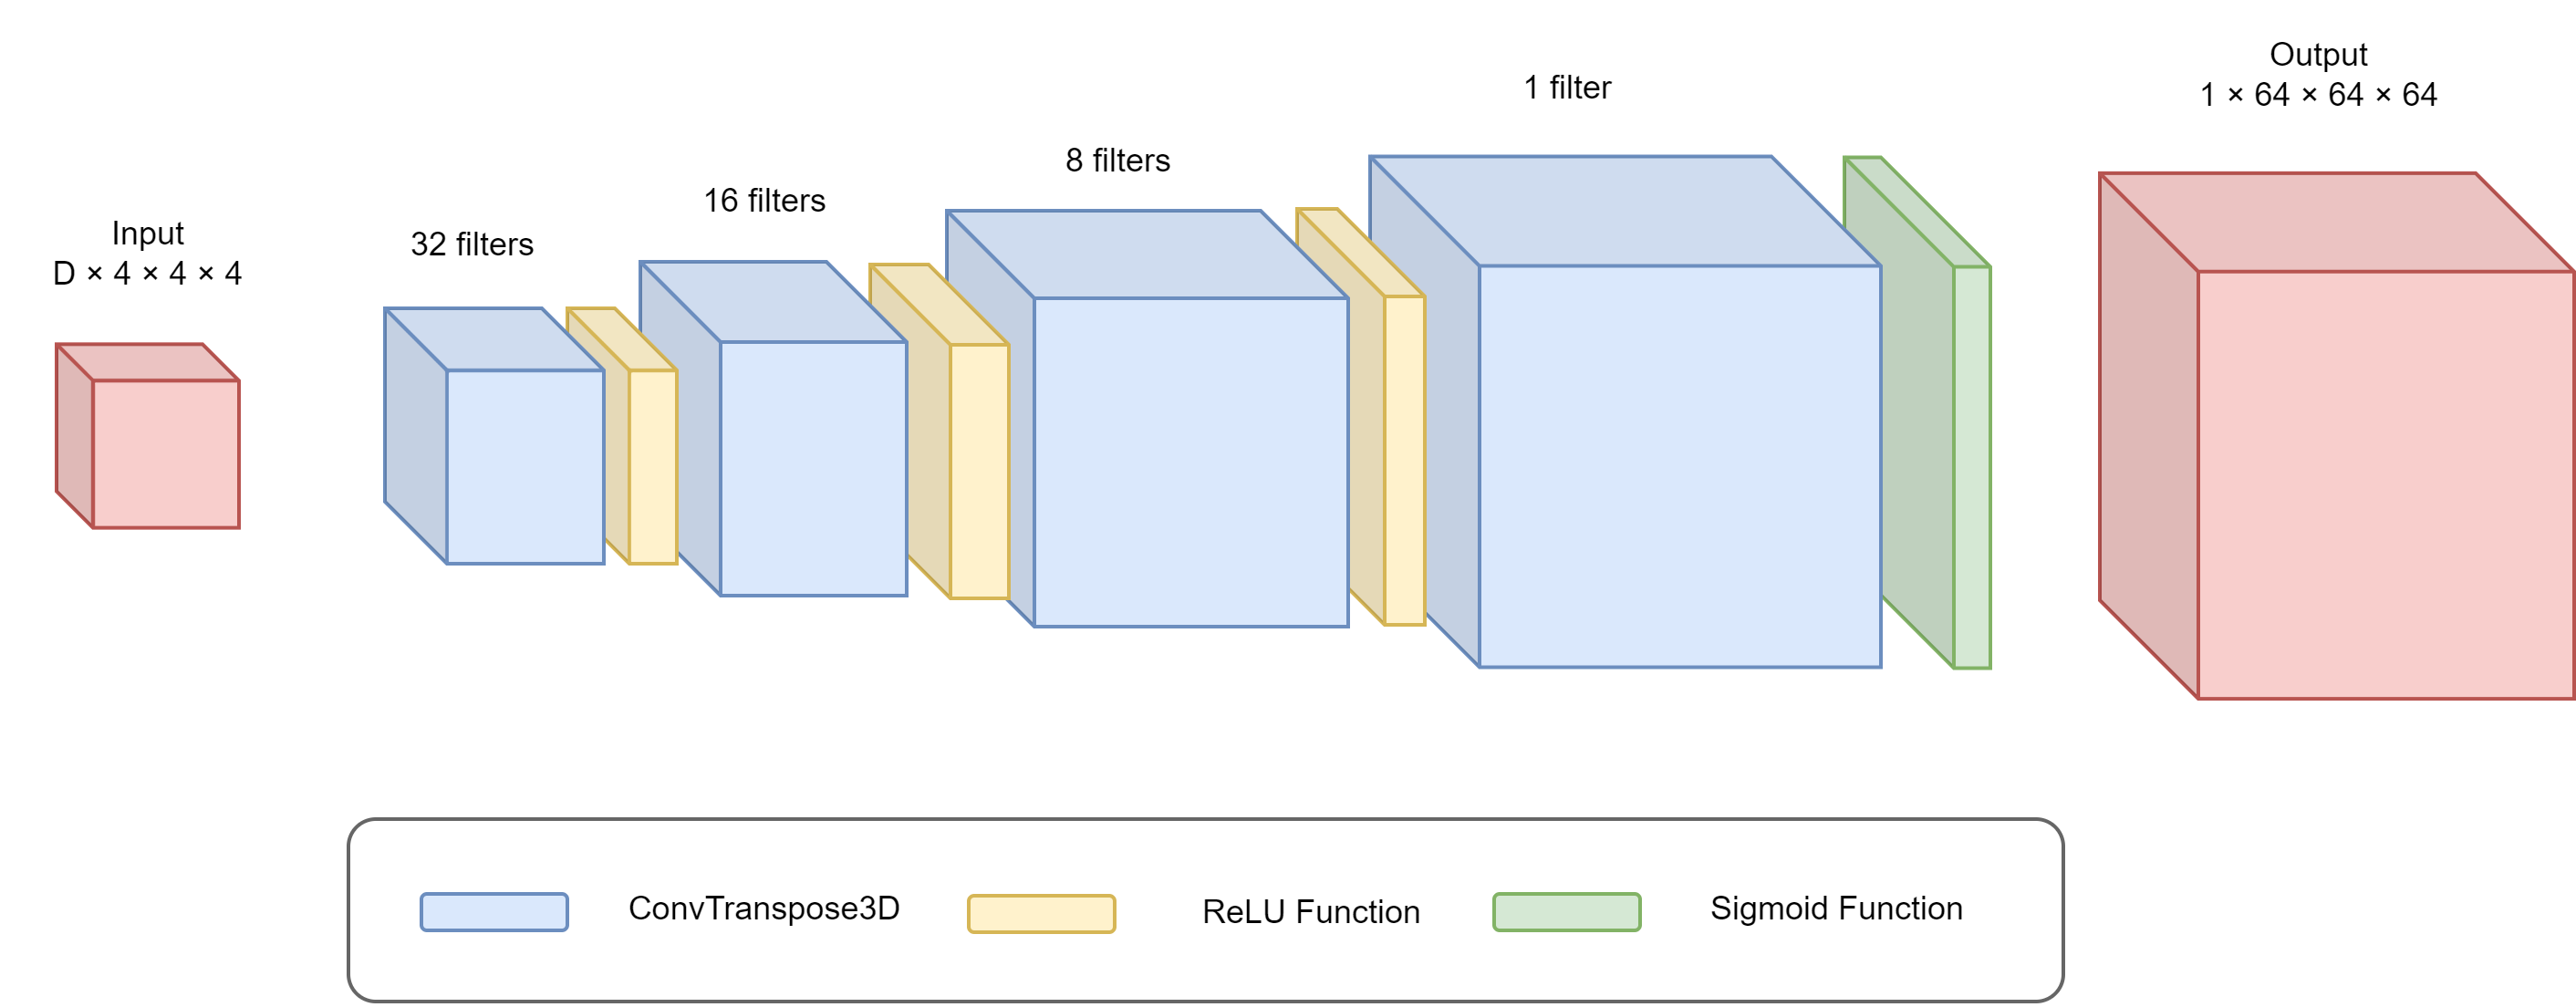
\includegraphics[width=\linewidth]{upscaler}
\caption{Architecture of the 3D upscaler module.}
\label{fig:upscaler}
\end{figure}

The input of the upscaler is the reshaped output of the 3D transformer decoder, since we need to transform the data from 2 dimensions into 4. In particular, the initial output of the decoder which is $4^3 \times D$ becomes our new input of the upscaler with size $D \times 4 \times 4 \times 4$.
The 3D upscaler is composed by four 3D transposed convolutional layers; the first three are followed by a ReLU activation function and the final one is followed by a sigmoid activation function. The number of filters applied by the convolutional layers decreases each time by a scale factor of 2. The first layer has 32 filters, the second one 16, then 8 and finally we have a single filter to produce only one output channel in the final voxel grid. The kernel size and stride value are set respectively to 4 and 2, upscaling the voxel grid received in input each time by a scale factor of 2. In Table \ref{tab:shapes} a summary of the shapes produced by each stage of the architecture is reported.

\begin{table}[h!]
\centering
\begin{tabular}{|c|c|c|}
\hline
Stage & Input Shape & Output Shape \\
\hline\hline
Linear Projection & $2 \times P \times K$ & $2 \times P \times E$ \\
\hline
Tanh & $2 \times P \times E$ & $2 \times P \times E$ \\
\hline
Reshape & $2 \times P \times E$ & $(2 * P) \times E$ \\
\hline
2D Transformer Encoder & $(2 * P) \times E$ & $(2 * P) \times E$ \\
\hline
Linear Projection & $(2 * P) \times E$ & $(2 * P) \times D$ \\
\hline
Tanh & $(2 * P) \times D$ & $(2 * P) \times D$ \\
\hline
3D Transformer Decoder & $(2 * P) \times D \, || \, 4^3 \times D$ & $4^3 \times D$ \\
\hline
Reshape & $4^3 \times D$ & $D \times 4 \times 4 \times 4$ \\
\hline
3D Upscaler & $D \times 4 \times 4 \times 4$ & $1 \times 64 \times 64 \times 64$ \\
\hline
\end{tabular}
\caption{Table reporting the input and output shape for each stage of the architecture.}
\label{tab:shapes}
\end{table}

\subsection{Loss function}

In the literature for 3D reconstruction the cross-entropy loss is generally used, but as stated in \cite{3d-retr} the Dice loss is more suited for tasks in which the IoU metric is optimized. Therefore, the loss function used for this architecture is the Dice loss.

Formally, the Dice loss can be defined in the following way:
\begin{equation}
DiceLoss(p_i, g_i) = 1 - \frac{2 \sum_{j=1}^N p_{i,j} g_{i,j}}{\sum_{j=1}^N p_{i,j}^2 + \sum_{j=1}^N g_{i,j}^2},
\end{equation}
where $p_i$ and $g_i$ are respectively the flattened version of the model predictions $\hat{y}_i$ and the ground truth grids $y_i$. In particular, each voxel grid of shape $64 \times 64 \times 64$ is reshaped into a vector of size $64^3$.


\chapter{Experimental Results}\label{cap:results}

In this chapter the results obtained with the method proposed will be illustrated and discussed in Section \ref{sec:eval}, both from a qualitative and quantitative point of view. In Section \ref{sec:dataset} the procedure used for the collection and creation of the dataset will be illustrated. Moreover, in Section \ref{sec:csi-eval} a first visual evaluation of the amplitude and phase as processed by the sanitization phase will be shown. Finally, in Section \ref{sec:ablation} the ablation studies will be described.

\section{Dataset}\label{sec:dataset}

One of the major contributions of this thesis is a new dataset collected specifically for the task of environment reconstruction starting from CSI data. In particular, 100 CSI samples composed by 512 packets each was collected for 8 rooms, for a total of 800 CSI samples and more than 400.000 exchanged packets.

In the following the methodology used in order to collect this data will be described.

\subsection{CSI Data}

The input of this task is CSI data which can be collected relying standard Wi-Fi protocols. In order to collect this data an integrated chip was used for both transmitter and receiver. One of the best fit for the need of this thesis was the ESP32, shown in Figure \ref{fig:esp32}, which is a low-cost and low-power device with integrated Wi-Fi communication.

\begin{figure}[h!]
\centering
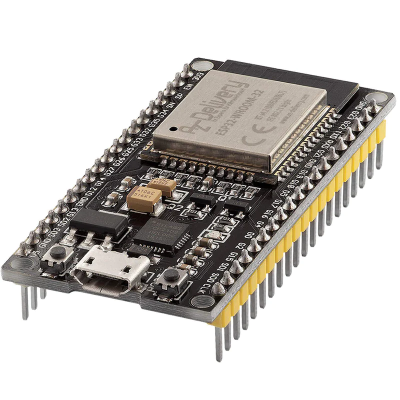
\includegraphics[width=.25\linewidth]{esp32}
\caption{Photo of a ESP32 module.}
\label{fig:esp32}
\end{figure}

For the number of receivers $NRX$ and transmitters $NTX$ only one device was used for each role, i.e. $NRX = NTX = 1$. So, two ESP32 modules were used after the needed configuration: one as router (AP) and the other as station (STA). These kind of devices are able to communicate using Wi-Fi protocols but they are not able to collect CSI measurements by default.
In fact, for this intent an external software tool was used, available at \url{https://github.com/StevenMHernandez/ESP32-CSI-Tool}. This tool enabled to store CSI data and other information about the communication in a simple CSV file.

In order to collect samples for a new room, the two devices were placed on the diagonal of the room at least 3 meters apart, like shown in Figure \ref{fig:devices-location}.

\begin{figure}[h!]
\centering
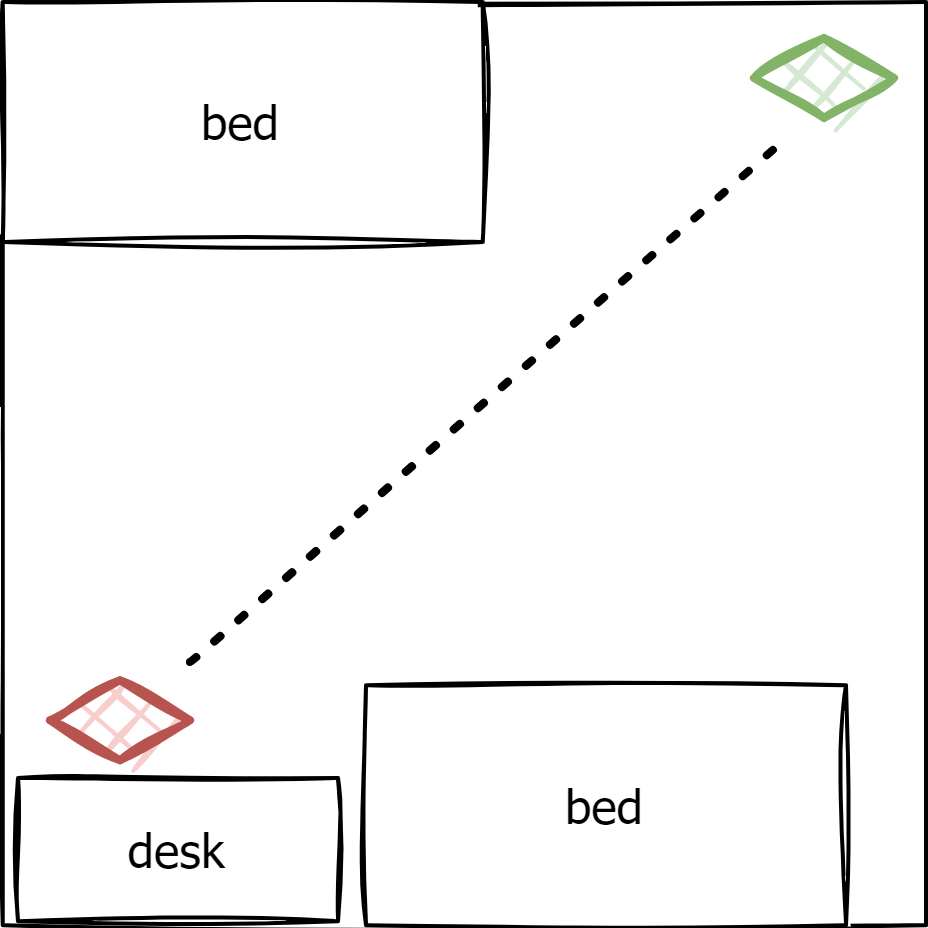
\includegraphics[width=.4\linewidth]{devices-location}
\caption{Graphical representation of the location of the two devices.}
\label{fig:devices-location}
\end{figure}

Then, the experiments were performed automatically using a custom script written in Python which collected all the CSI data produced during the experiments on the STA device in a separate CSV file for each experiment. The produced files can then be easily read and processed accordingly to compose the input of our dataset for this task.

\subsection{3D Models}

Collecting the CSI data is not enough in order to compose our dataset, in fact the CSI data represent only the input of it and in order to use Deep Learning techniques we need also a ground truth. In this case, the ground truth is composed by the 3D voxel representation of the room in which the experiments were performed. One of the major challenges of this thesis was to reconstruct the room with a sufficient number of details that a model could reproduce starting from the CSI data collected.

So, for each room all the bigger furniture were measured and reproduced in a voxel space $64 \times 64 \times 64$ using as unit measure 1 voxel = $10 \times 10 \times 10$ cm. Thus, the maximum width, height and depth of a room that can be represented is 6 meters and 40 centimeters for each dimension.
A simple online voxel editor was used and the produced 3D models were saved in separate files with the coordinates of the occupied voxels. An example of the ground truth of the dataset is shown in Figure \ref{fig:room-example}.

\begin{figure}[h!]
\centering
\begin{subfigure}{.49\textwidth}
	\centering
	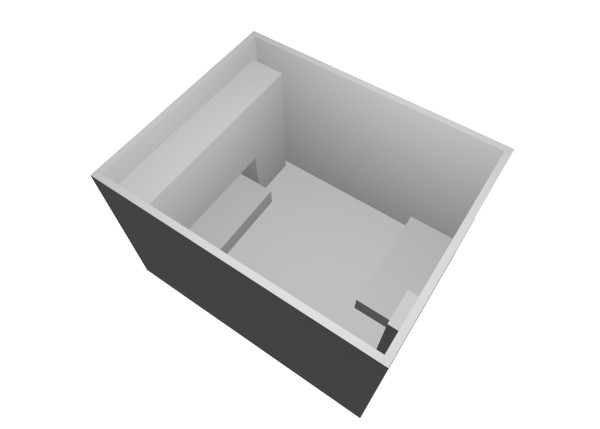
\includegraphics[width=\linewidth]{3d-example-1}
\end{subfigure}
\begin{subfigure}{.49\textwidth}
	\centering
	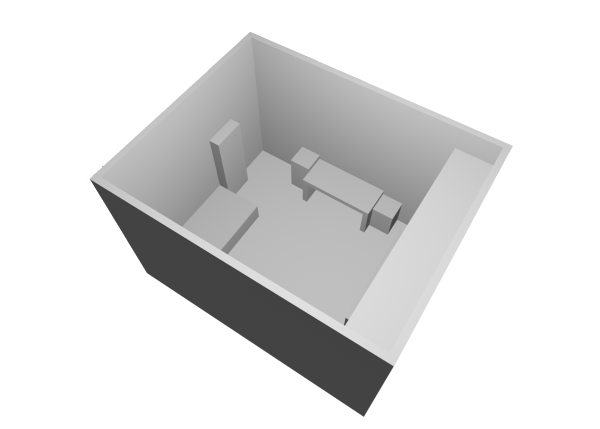
\includegraphics[width=\linewidth]{3d-example-2}
\end{subfigure}
\caption{Example of the same room represented using voxels from two different points of view.}
\label{fig:room-example}
\end{figure}

\section{CSI Processing Evaluation}\label{sec:csi-eval}

An initial evaluation of the results produced by the sanitization procedure, illustrated in Section \ref{sec:csi-san}, is presented in this section. There is no metric able to evaluate quantitatively the procedure applied, therefore a qualitative evaluation will be carried out. The sanitization procedure was performed using MATLAB, which is the software also used to generate the following plots. In Figure \ref{fig:amp-comp} a comparison among the different sanitized amplitude surfaces is shown. In the first row we have two samples from the same room and in the second row other two samples from another room. From the surfaces we can see that different rooms present slightly different surfaces, showing that amplitude is in fact affected by the environment, in particular by objects present in the room. However, even if the surfaces from distinct rooms are different, a human would not be able to determine which objects affected in which way the surface shape.

Instead, in Figure \ref{fig:phase-comp} a comparison among the different phase plots after the sanitization step is shown. In contrast to the amplitude, the phase is more difficult to interpret by simply looking at the plots. We can notice that in the first row the values are in a smaller range with respect to the values in the plots of the second row. However, looking at the distribution of the data, the phase doesn't seem to show a very good discriminative power for environments, but of course a model could identify patterns that from a human point of view are not so highlighted. More about the impact of amplitude and phase will be described in Section \ref{sec:ablation}.

\begin{figure}[h!]
\centering
\begin{subfigure}{.49\textwidth}
	\centering
	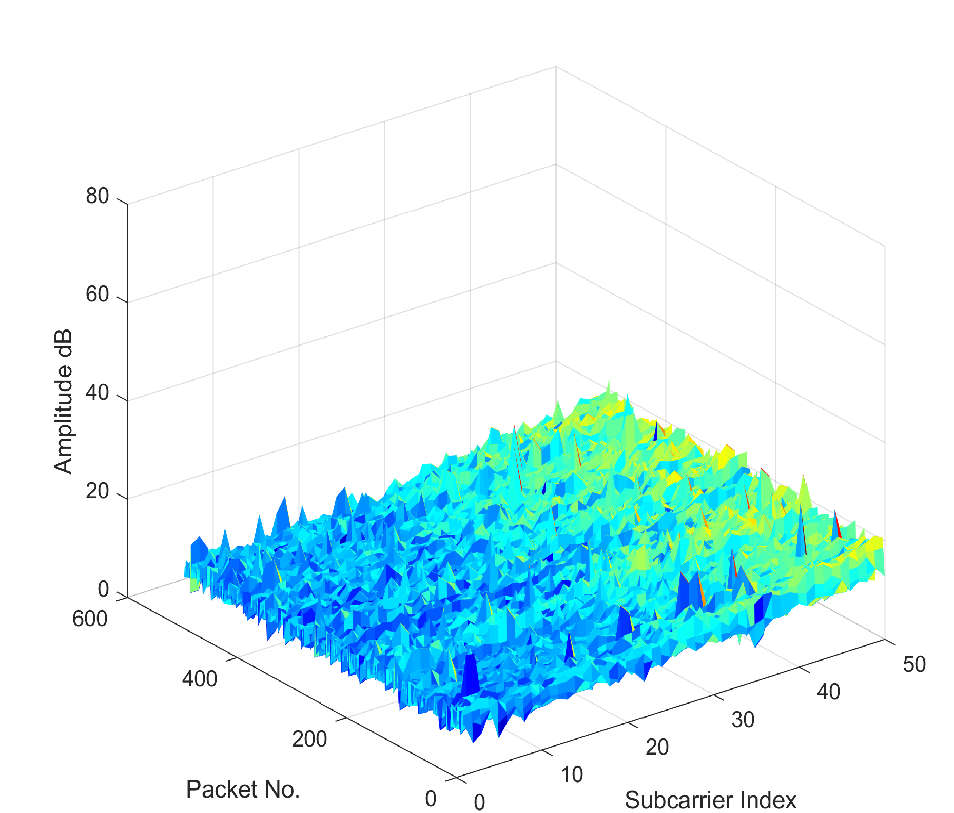
\includegraphics[width=.8\linewidth]{ce-v2-1}
	\caption{}
\end{subfigure}
\begin{subfigure}{.49\textwidth}
	\centering
	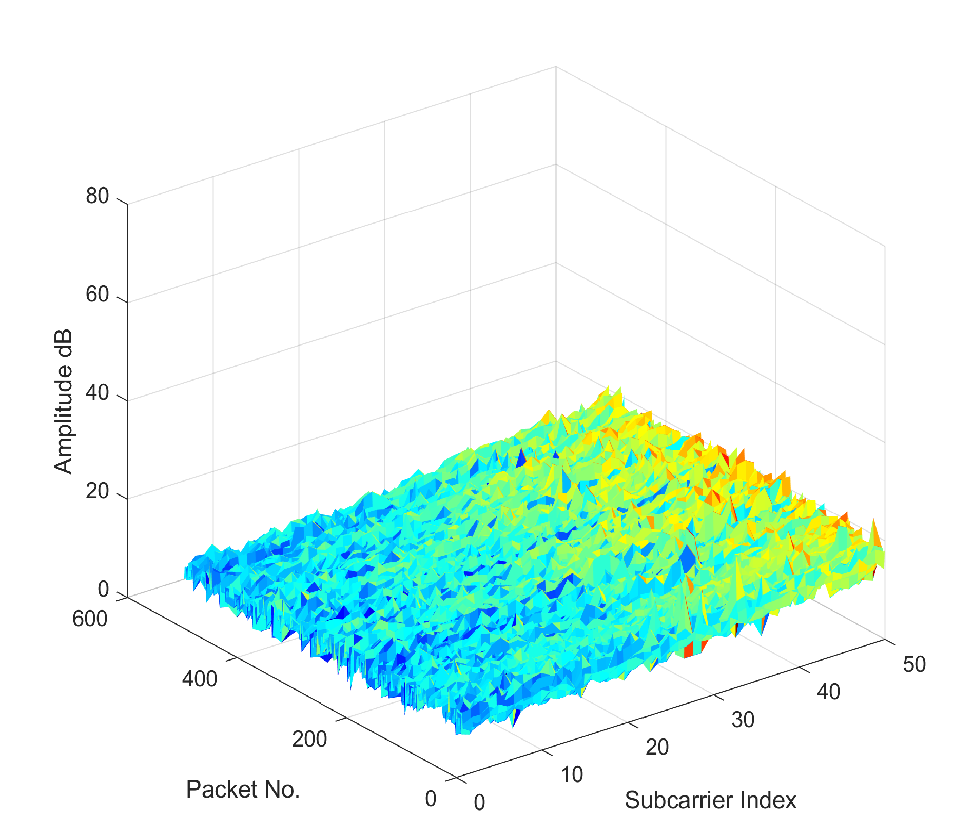
\includegraphics[width=.8\linewidth]{ce-v2-3}
	\caption{}
\end{subfigure}
\begin{subfigure}{.49\textwidth}
	\centering
	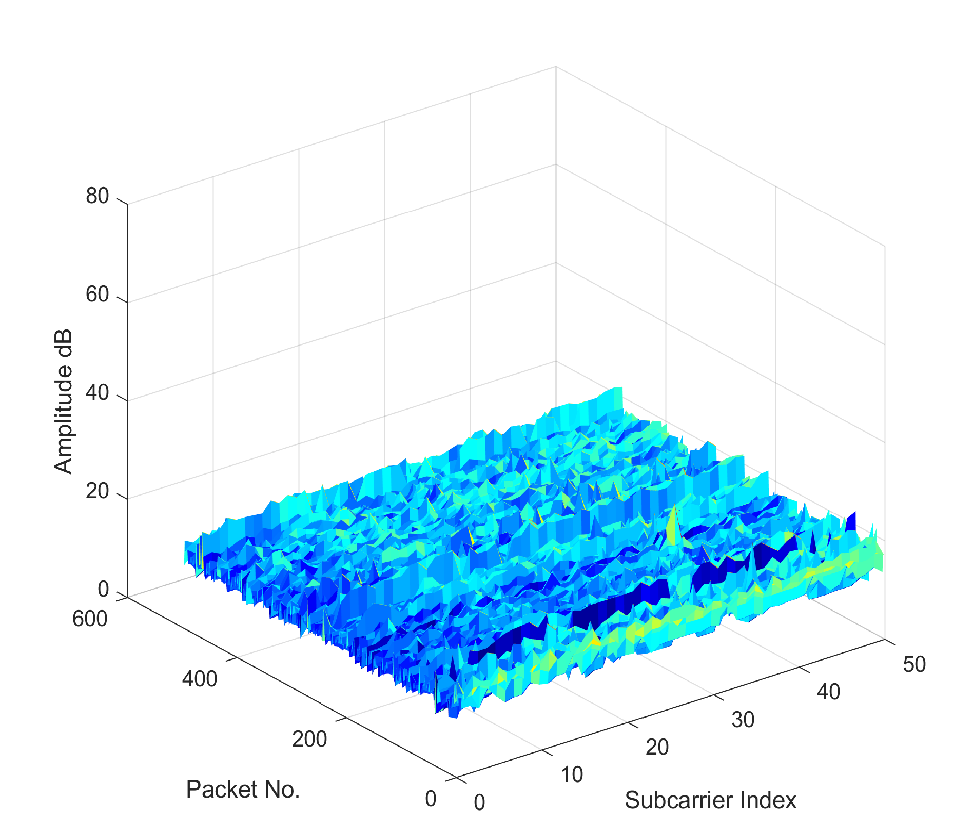
\includegraphics[width=.8\linewidth]{room2-v7-6}
	\caption{}
\end{subfigure}
\begin{subfigure}{.49\textwidth}
	\centering
	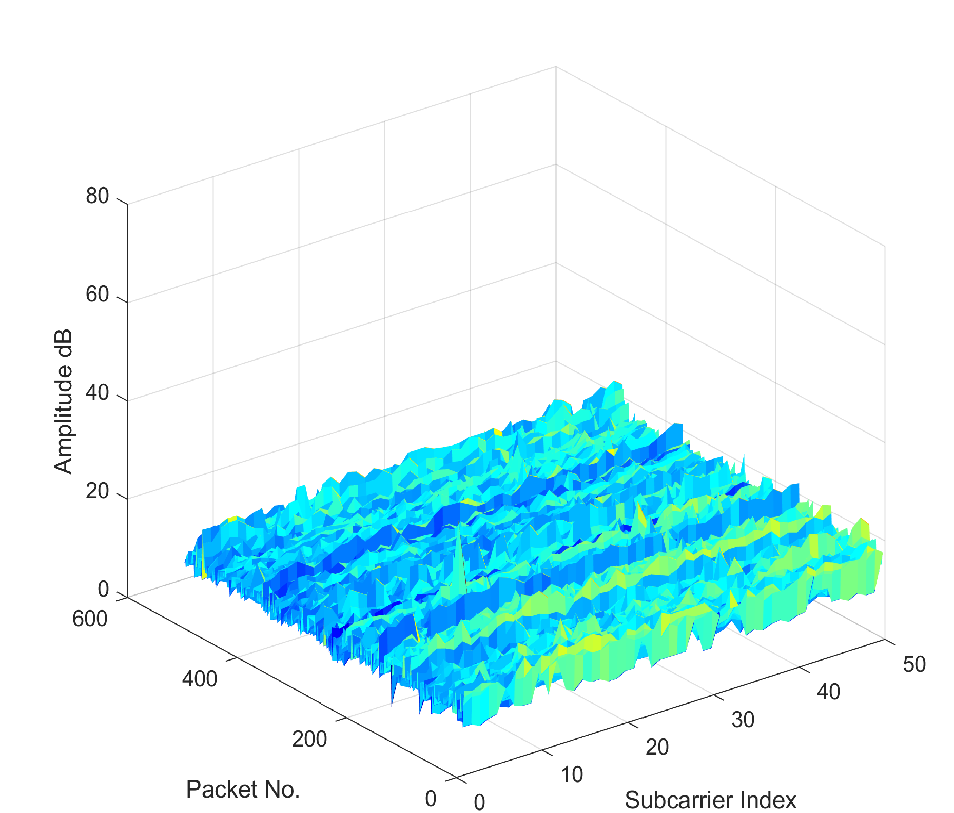
\includegraphics[width=.8\linewidth]{room2-v7-10}
	\caption{}
\end{subfigure}
\caption{Visual comparison of the collected sanitized amplitude for each packet and subcarrier from different rooms. The samples (a) and (b) are from the same room, instead (c) and (d) are from another room.}
\label{fig:amp-comp}
\end{figure}

\begin{figure}[h!]
\centering
\begin{subfigure}{.49\textwidth}
	\centering
	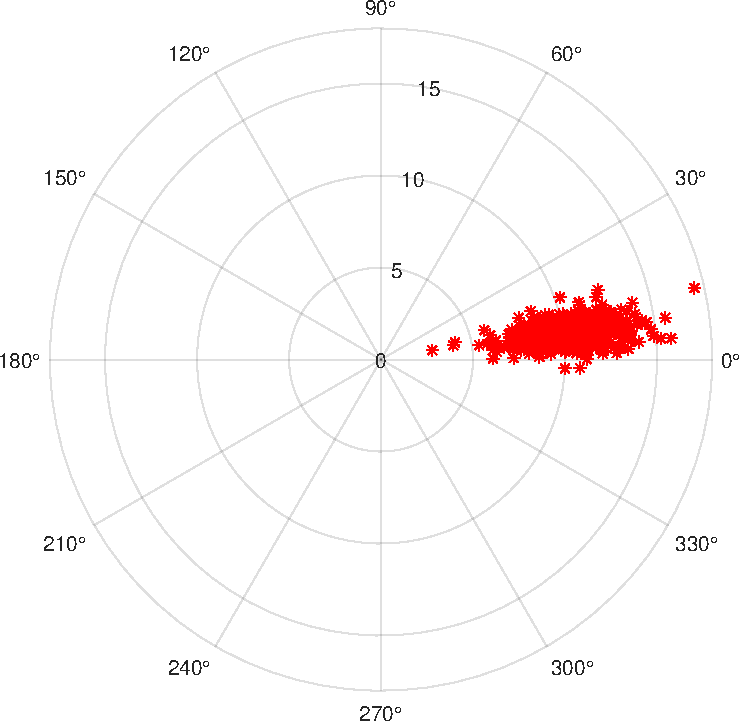
\includegraphics[width=.7\linewidth]{ce-v2-3-sanitized_phase subcarrier_1}
	\caption{}
\end{subfigure}
\begin{subfigure}{.49\textwidth}
	\centering
	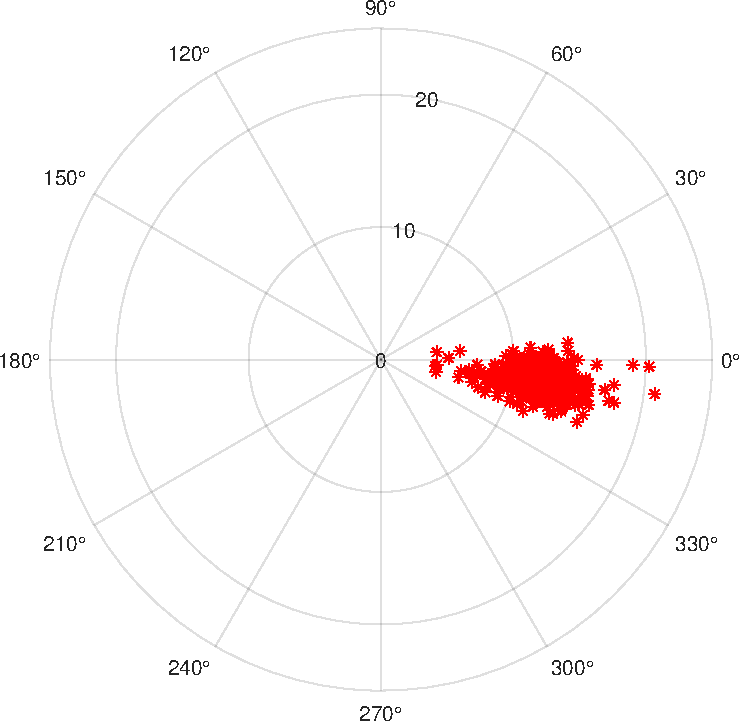
\includegraphics[width=.7\linewidth]{ce-v2-3-sanitized_phase subcarrier_21}
	\caption{}
\end{subfigure}
\begin{subfigure}{.49\textwidth}
	\centering
	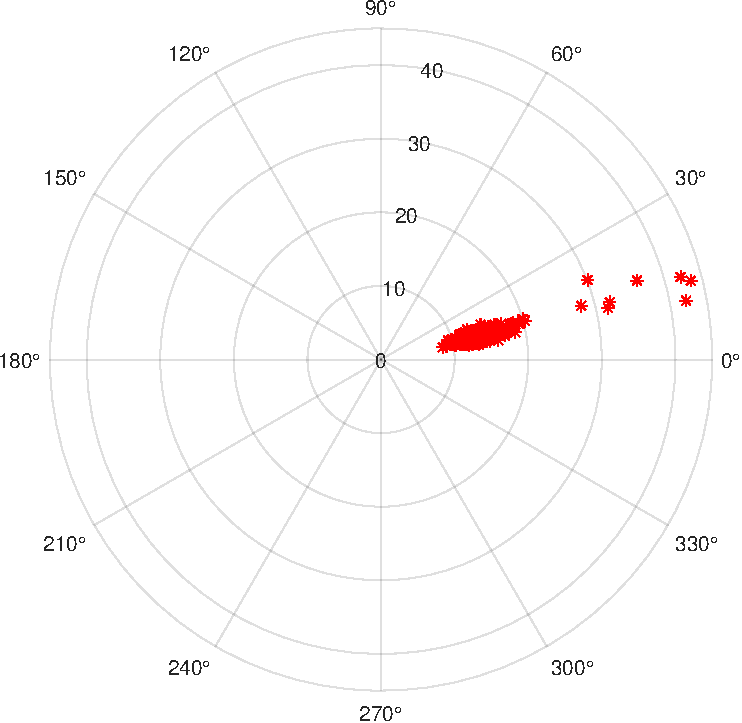
\includegraphics[width=.7\linewidth]{room2-v7-6-sanitized_phase subcarrier_1}
	\caption{}
\end{subfigure}
\begin{subfigure}{.49\textwidth}
	\centering
	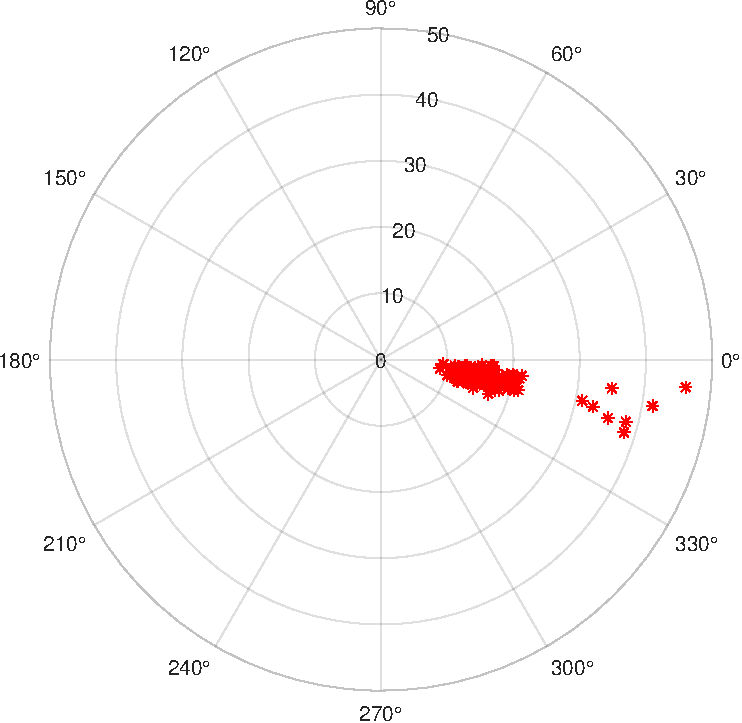
\includegraphics[width=.7\linewidth]{room2-v7-6-sanitized_phase subcarrier_21}
	\caption{}
\end{subfigure}
\caption{Visual comparison of the collected sanitized phase for each packet from different rooms. The samples (a) and (b) represent two different subcarriers from the same room, the same applies for (c) and (d) but they derive from another room.}
\label{fig:phase-comp}
\end{figure}

\section{Environment Reconstruction Evaluation}\label{sec:eval}

In this section the results produced by the proposed method will be presented from both a qualitative and quantitative point of view.
The architecture shown in Chapter \ref{cap:method} was implemented using Python with the popular Pytorch framework. Additionally, Pytorch Lightining and Weights and Biases were used in order to save and inspect the experiments results in a comprehensive way. Moreover, in order to visualize the 3D models in a Jupyter notebook a visualization tool was created using the popular JavaScript 3D framework Three.js.

The dataset collected as described above was divided into 60\% for the training set, 20\% for the validation set and 20\% for the test set. For the experiments, the model was trained for 250 epochs using the Adam optimizer \cite{adam} with a learning rate of 0.0001 and a batch size of 8. Regarding the model, both embedding dimensions of the two linear projections $E$ and $D$ were set to 64. Instead, the number of layers for encoder $L_e$ and decoder $L_d$ was set to 1 with 4 as the number of heads $H$. Additionally, the number of packets $P$ fed to the model was set to 64. Finally, all the experiments here reported were performed using the Google Colab environment with a Tesla T4 as GPU.

\subsection{Qualitative results}

The evaluation of the qualitative results is based on insights that we can obtain looking at the outputs produced by the model. Some 3D results of the method can be seen in Figure \ref{fig:3d-res}, showing that the proposed method is able to discriminate the different rooms with a very high accuracy and reconstruct the 3D indoor environment in which the CSI data was collected with high precision. As we can notice the major problem of the model is for the reconstruction of tables, this is easily explained by the fact that tables, in particular table legs, have a very low impact on the Wi-Fi signal since they are very thin and the plane is almost parallel to the signal traveling between the two devices.

\begin{figure}[h!]
\centering
\begin{subfigure}{.49\textwidth}
	\centering
	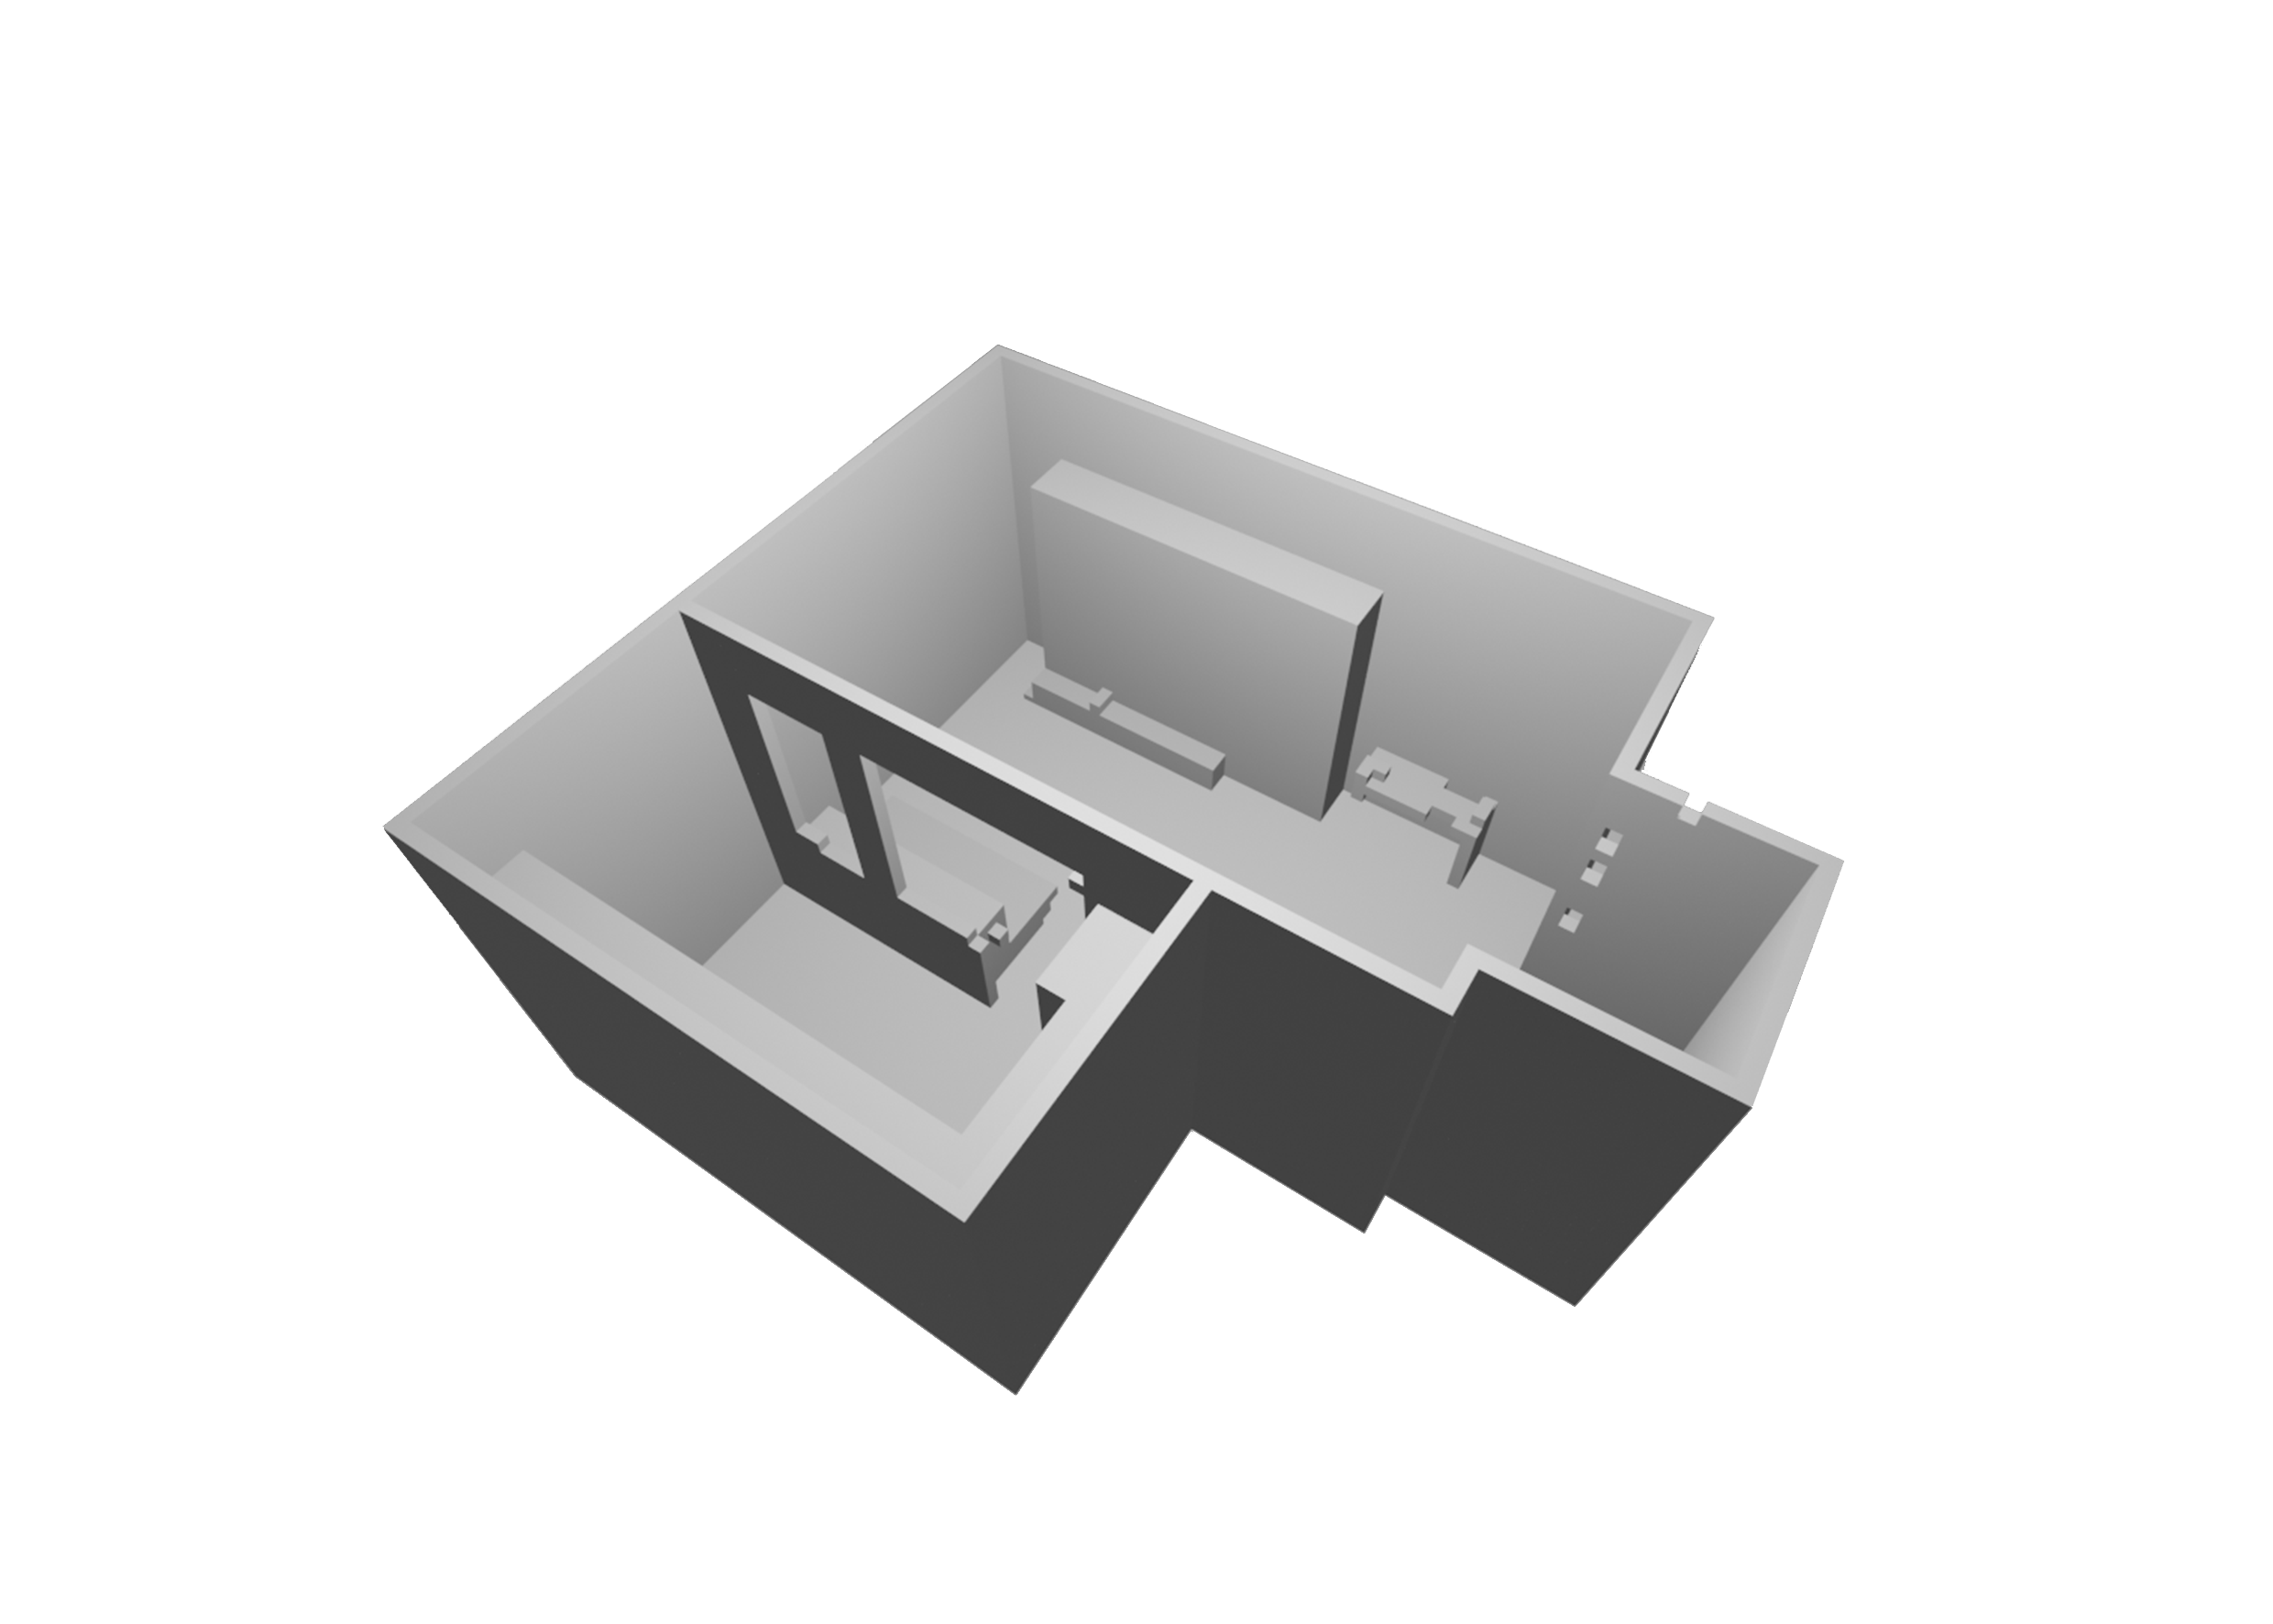
\includegraphics[width=.90\linewidth]{results/pred_0}
	\caption{}
\end{subfigure}
\begin{subfigure}{.49\textwidth}
	\centering
	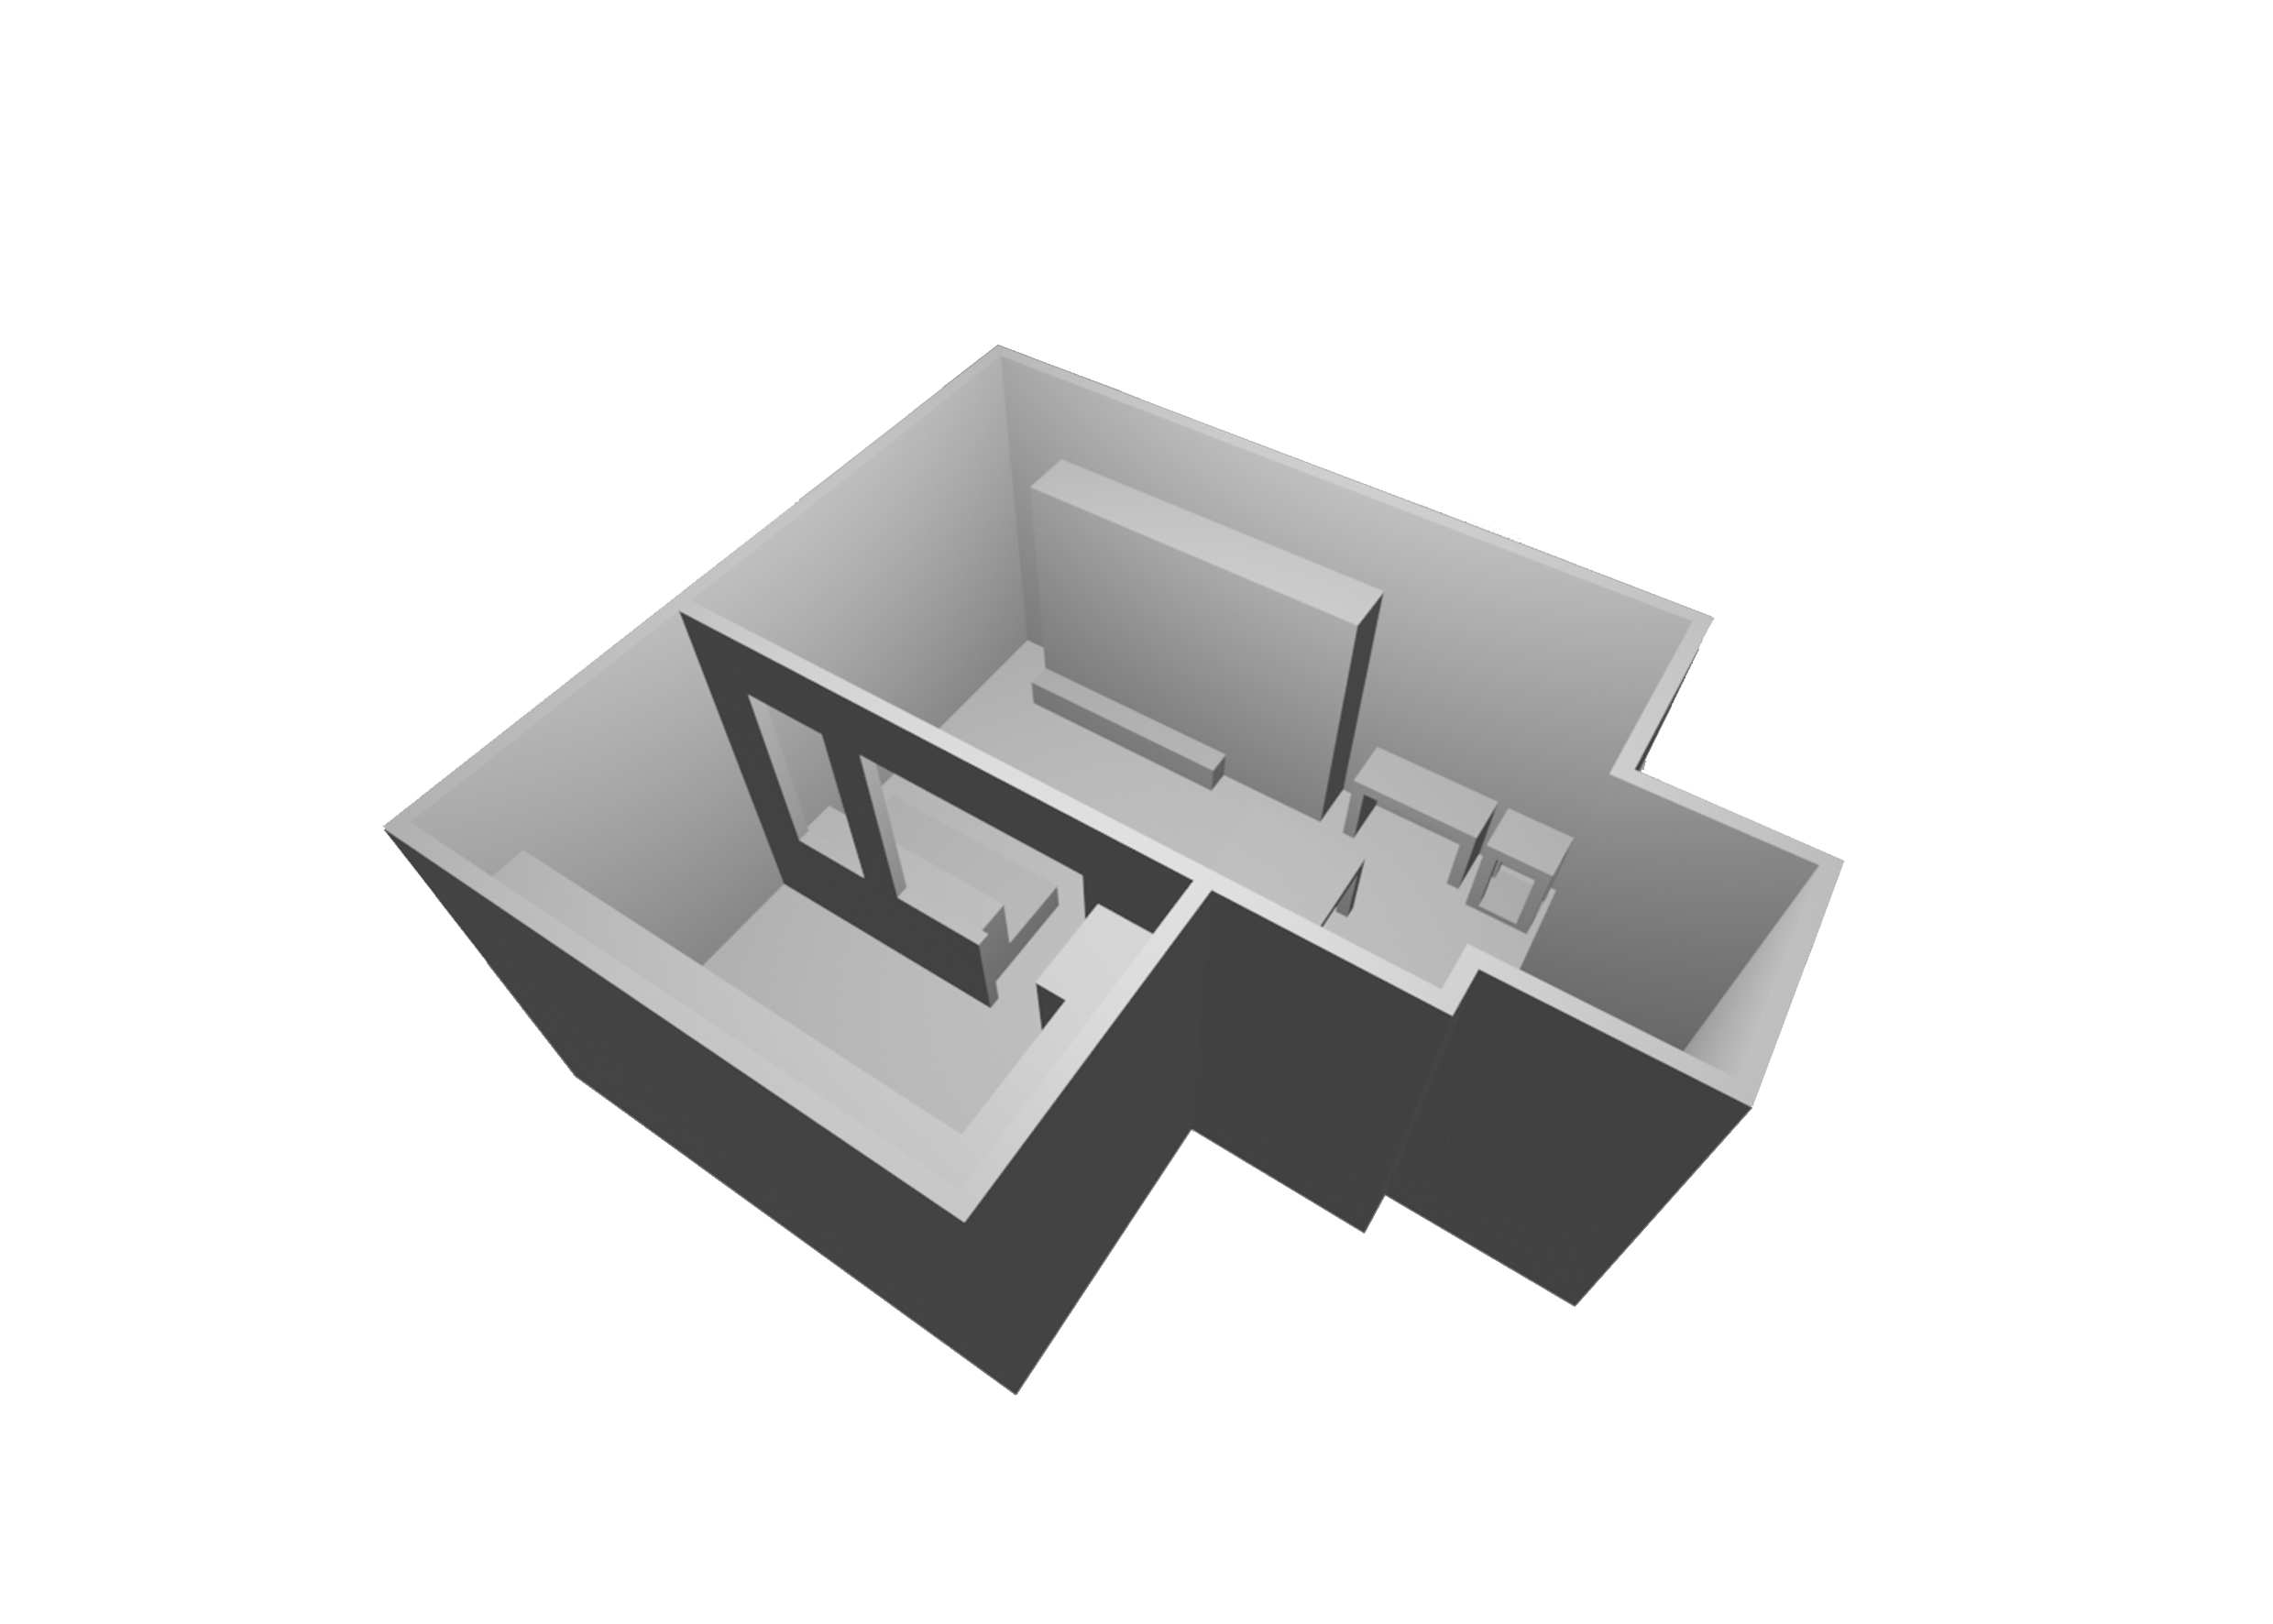
\includegraphics[width=.90\linewidth]{results/true_0}
	\caption{}
\end{subfigure}

\begin{subfigure}{.49\textwidth}
	\centering
	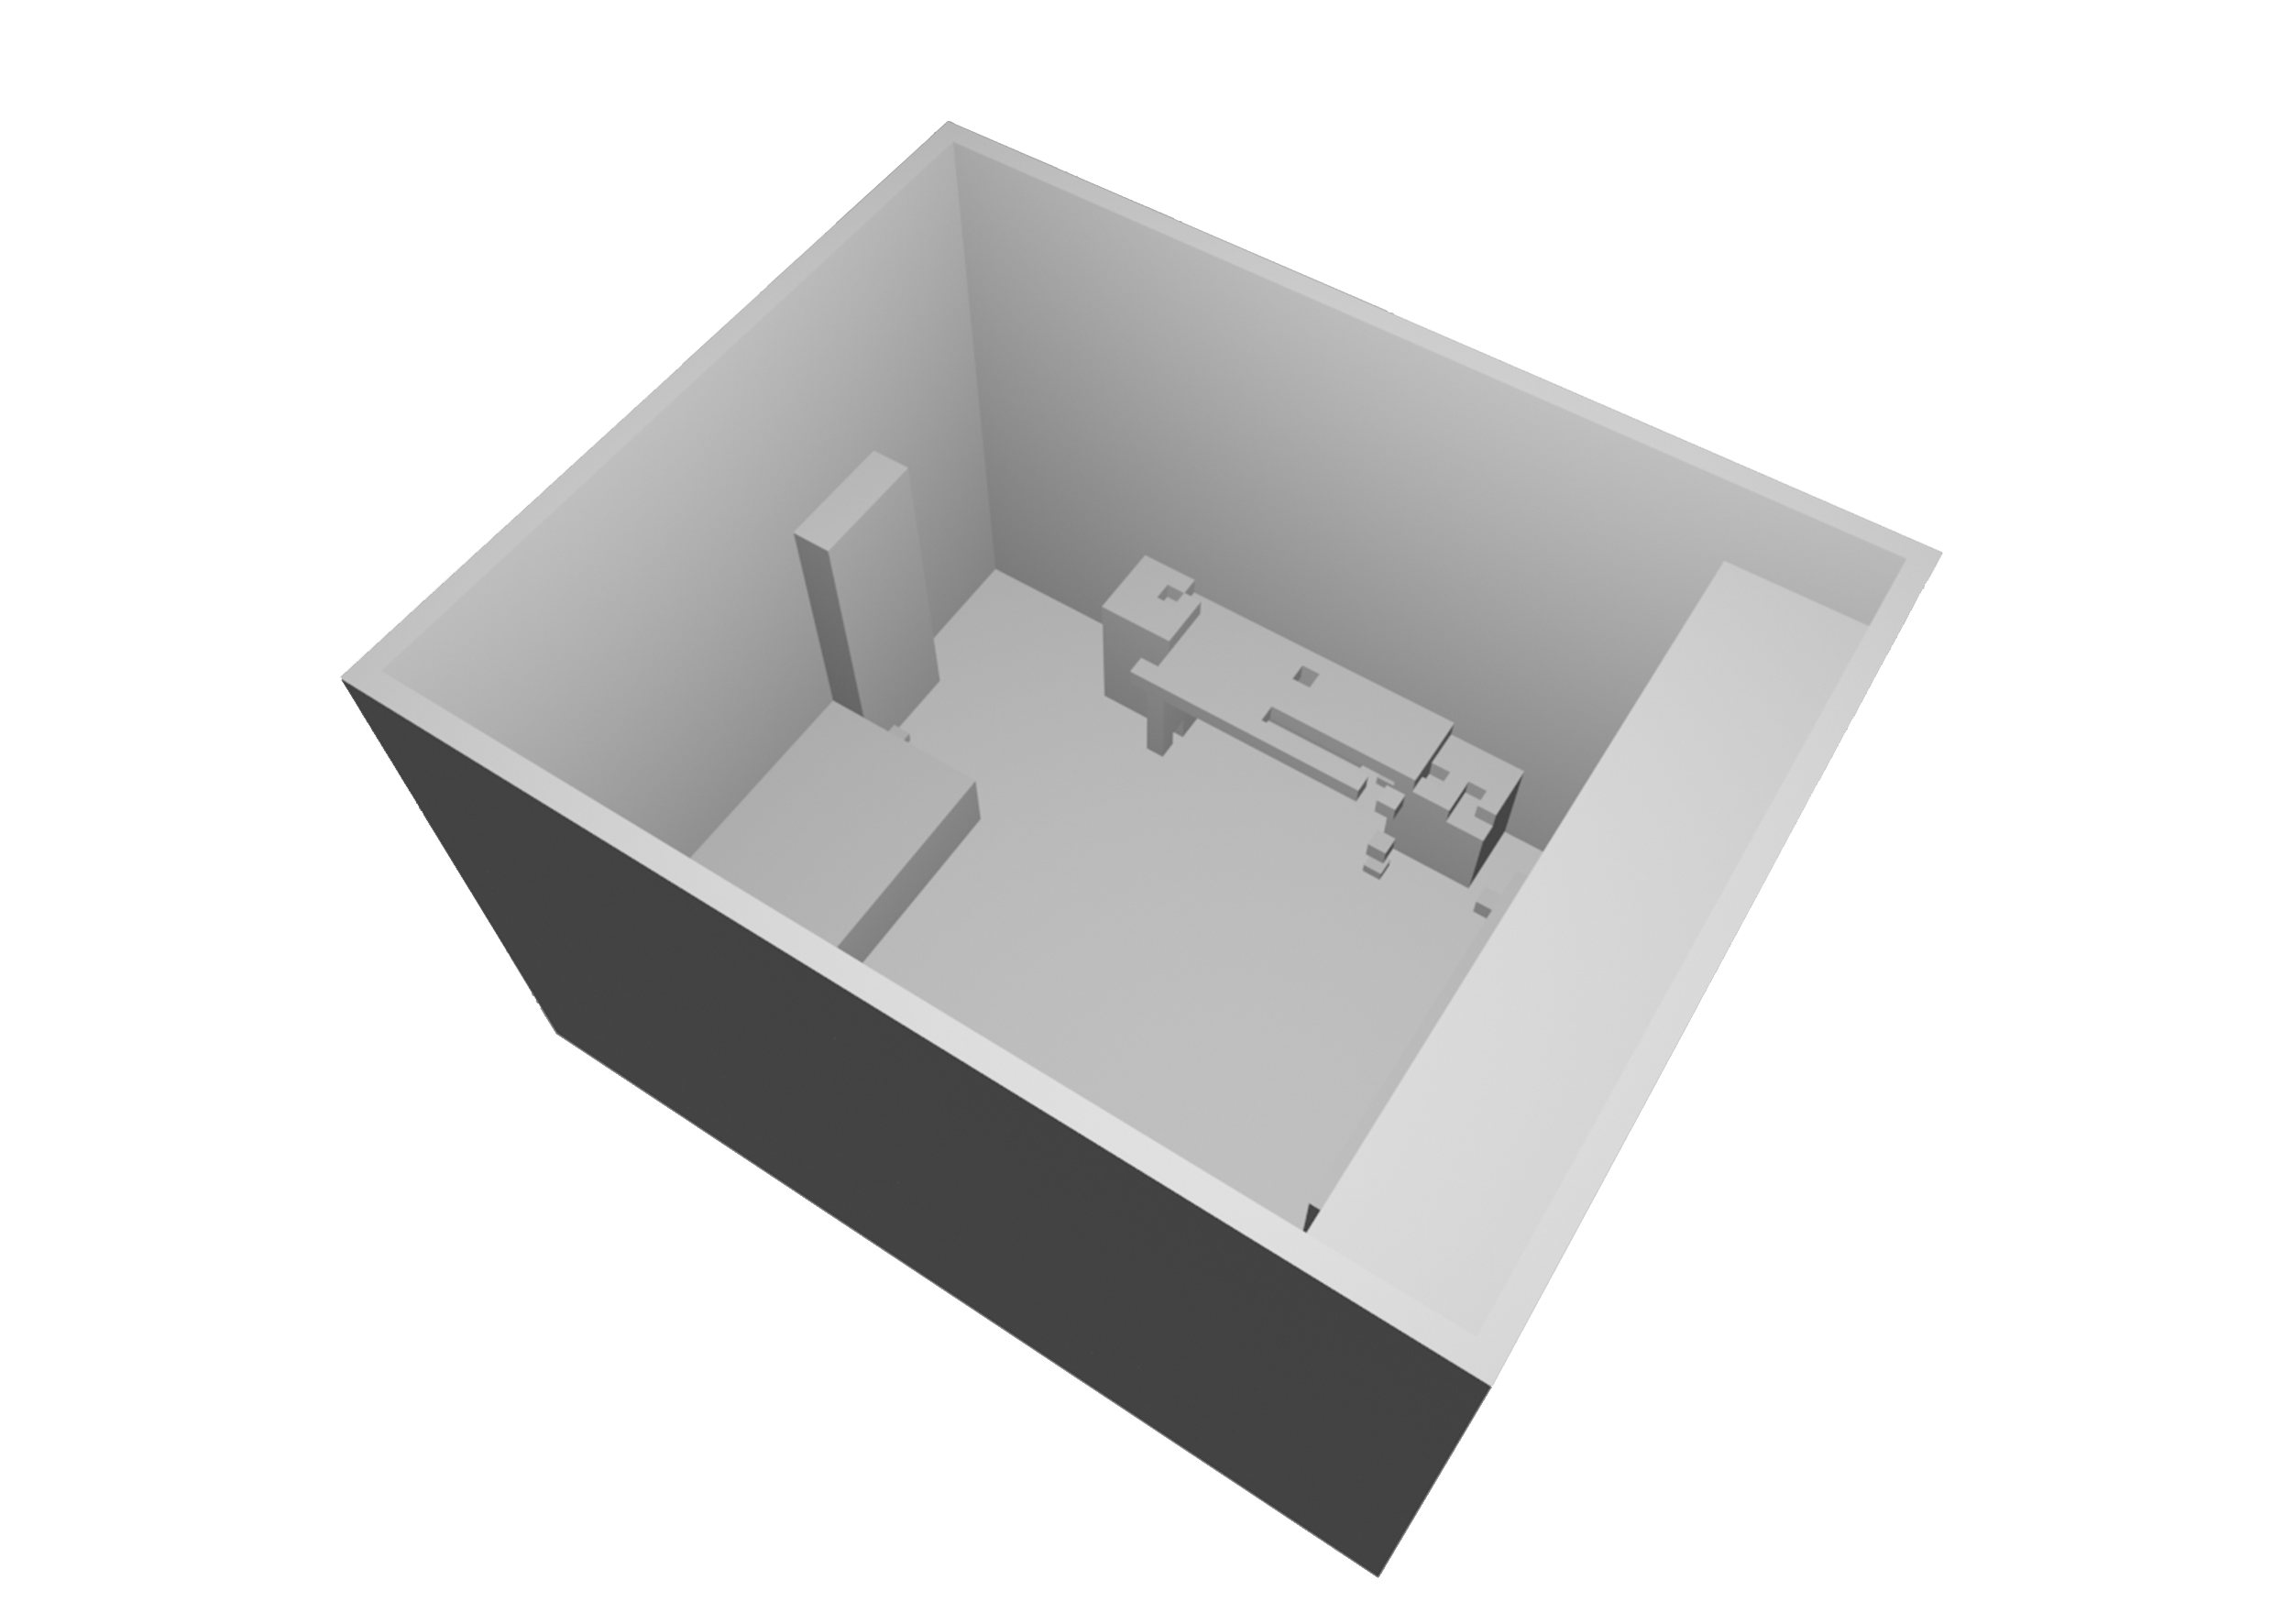
\includegraphics[width=.90\linewidth]{results/pred_1}
	\caption{}
\end{subfigure}
\begin{subfigure}{.49\textwidth}
	\centering
	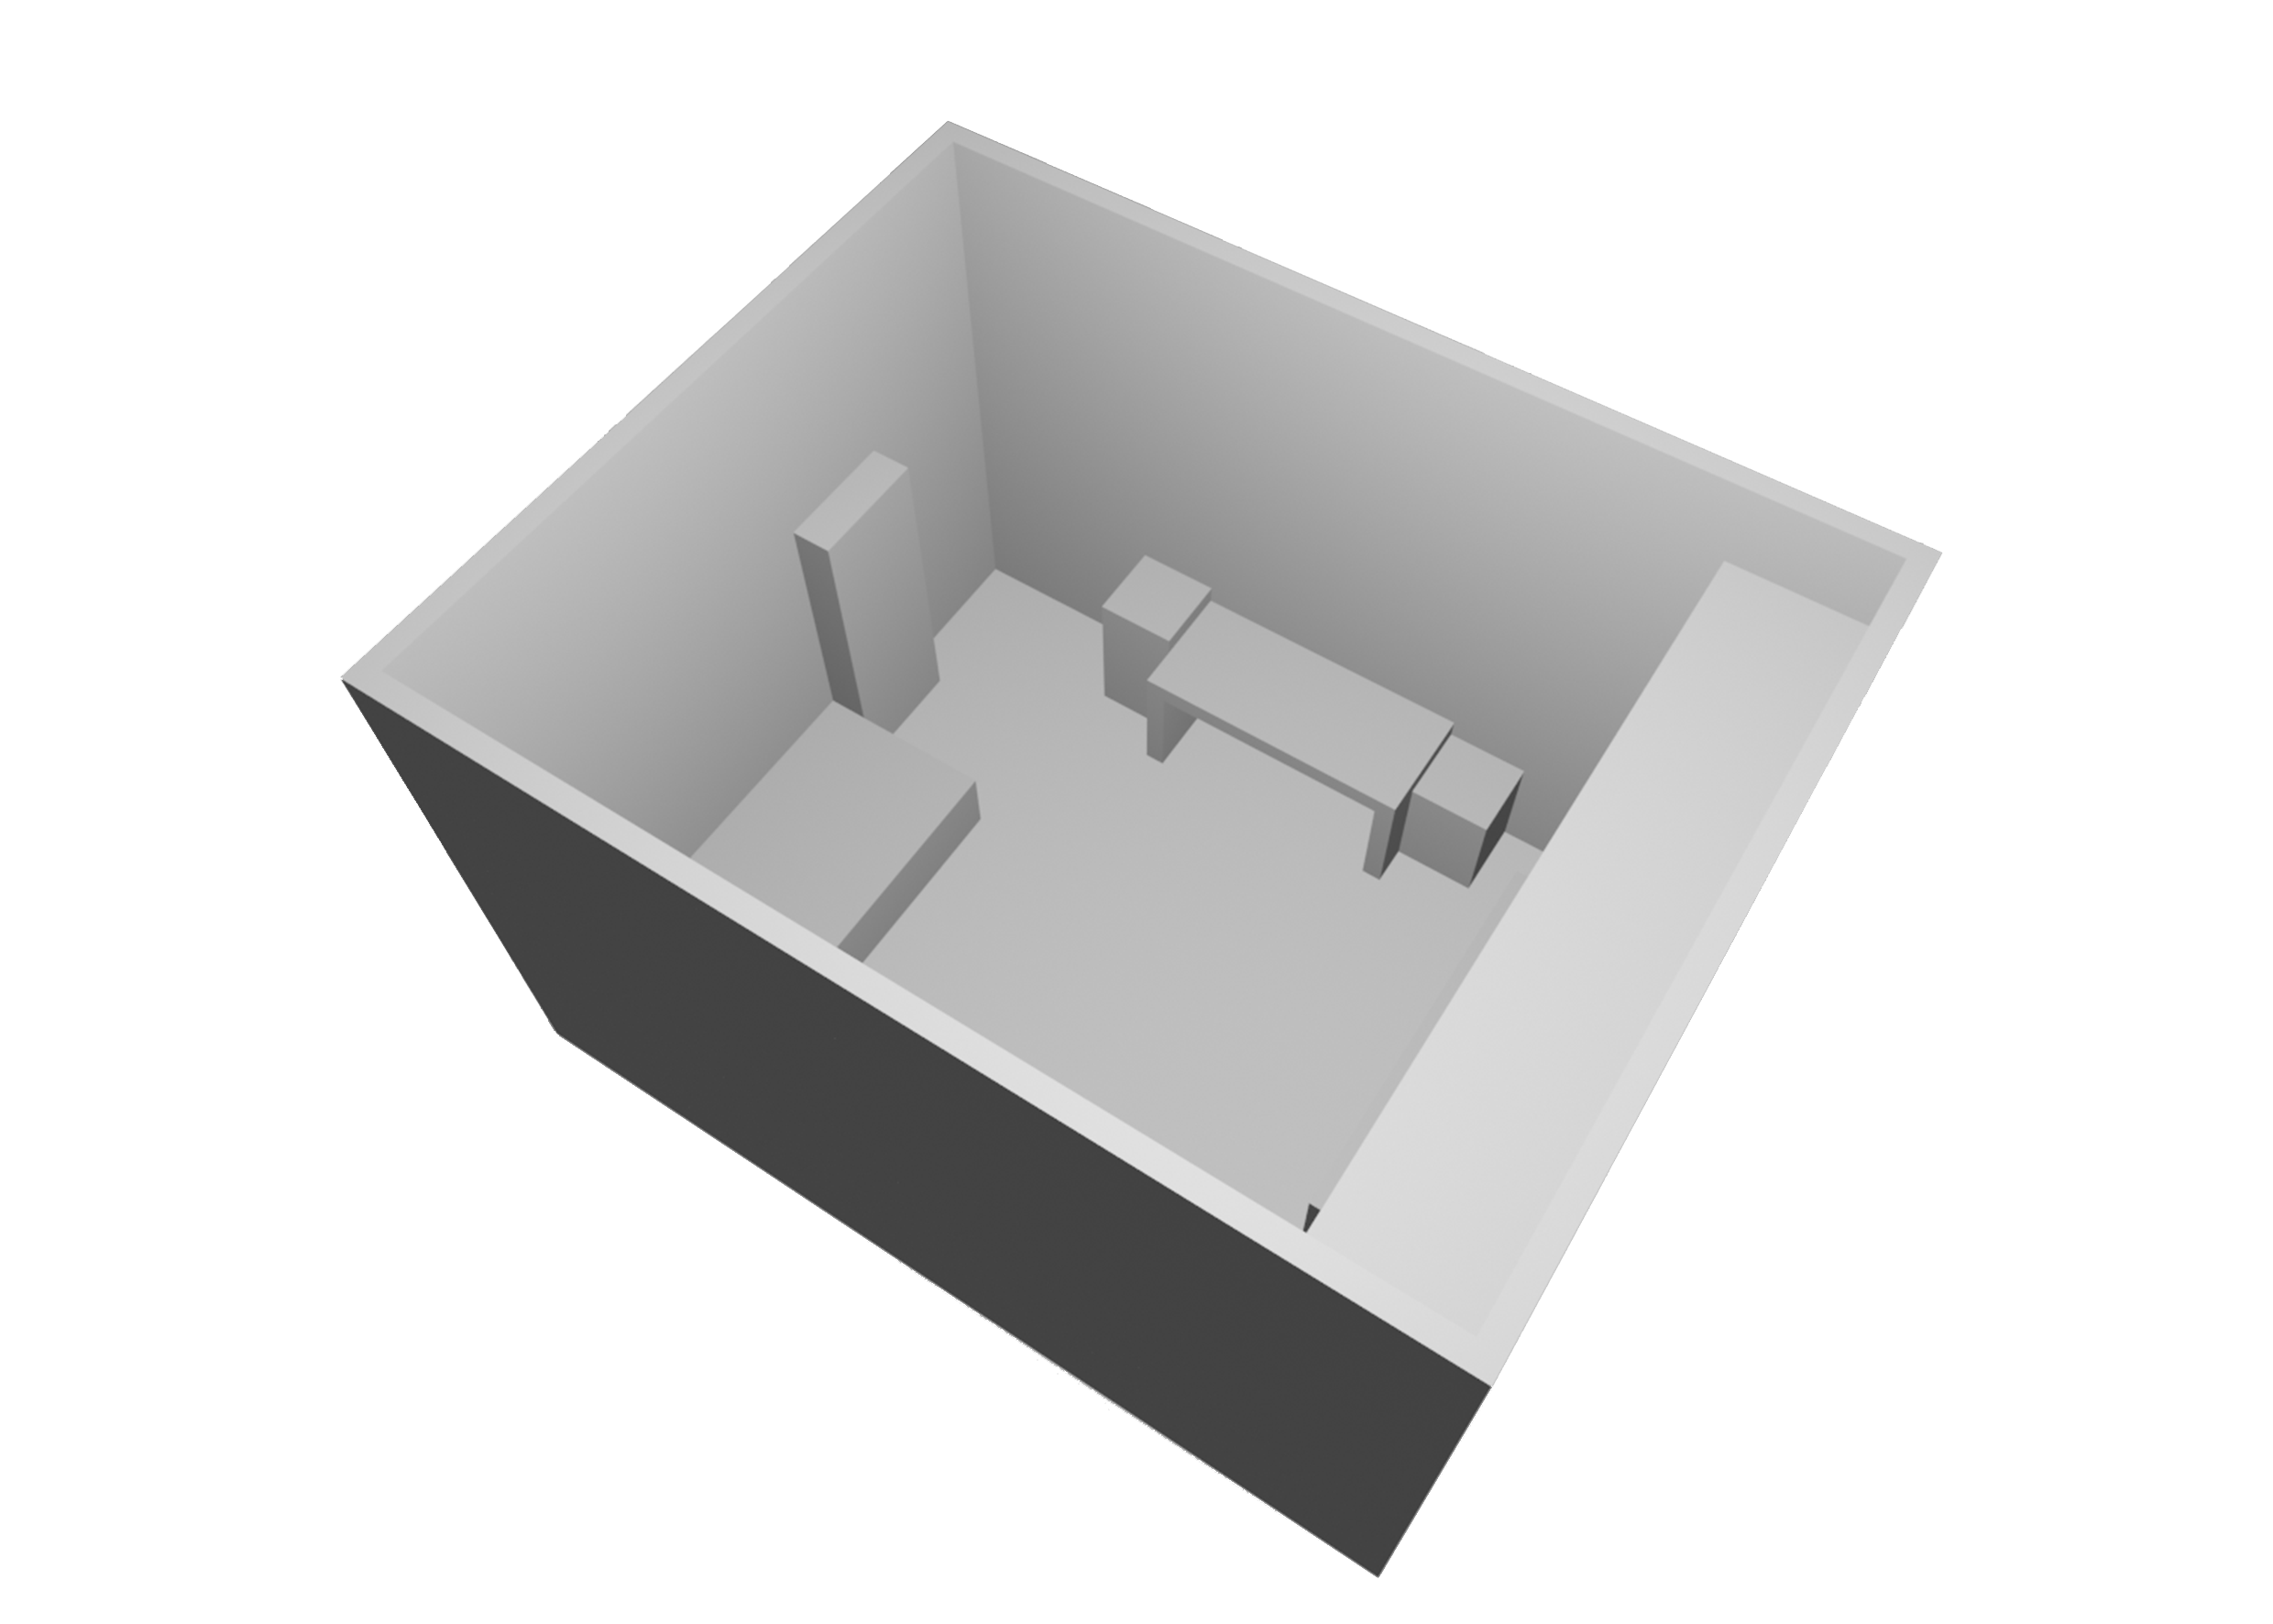
\includegraphics[width=.90\linewidth]{results/true_1}
	\caption{}
\end{subfigure}

\begin{subfigure}{.49\textwidth}
	\centering
	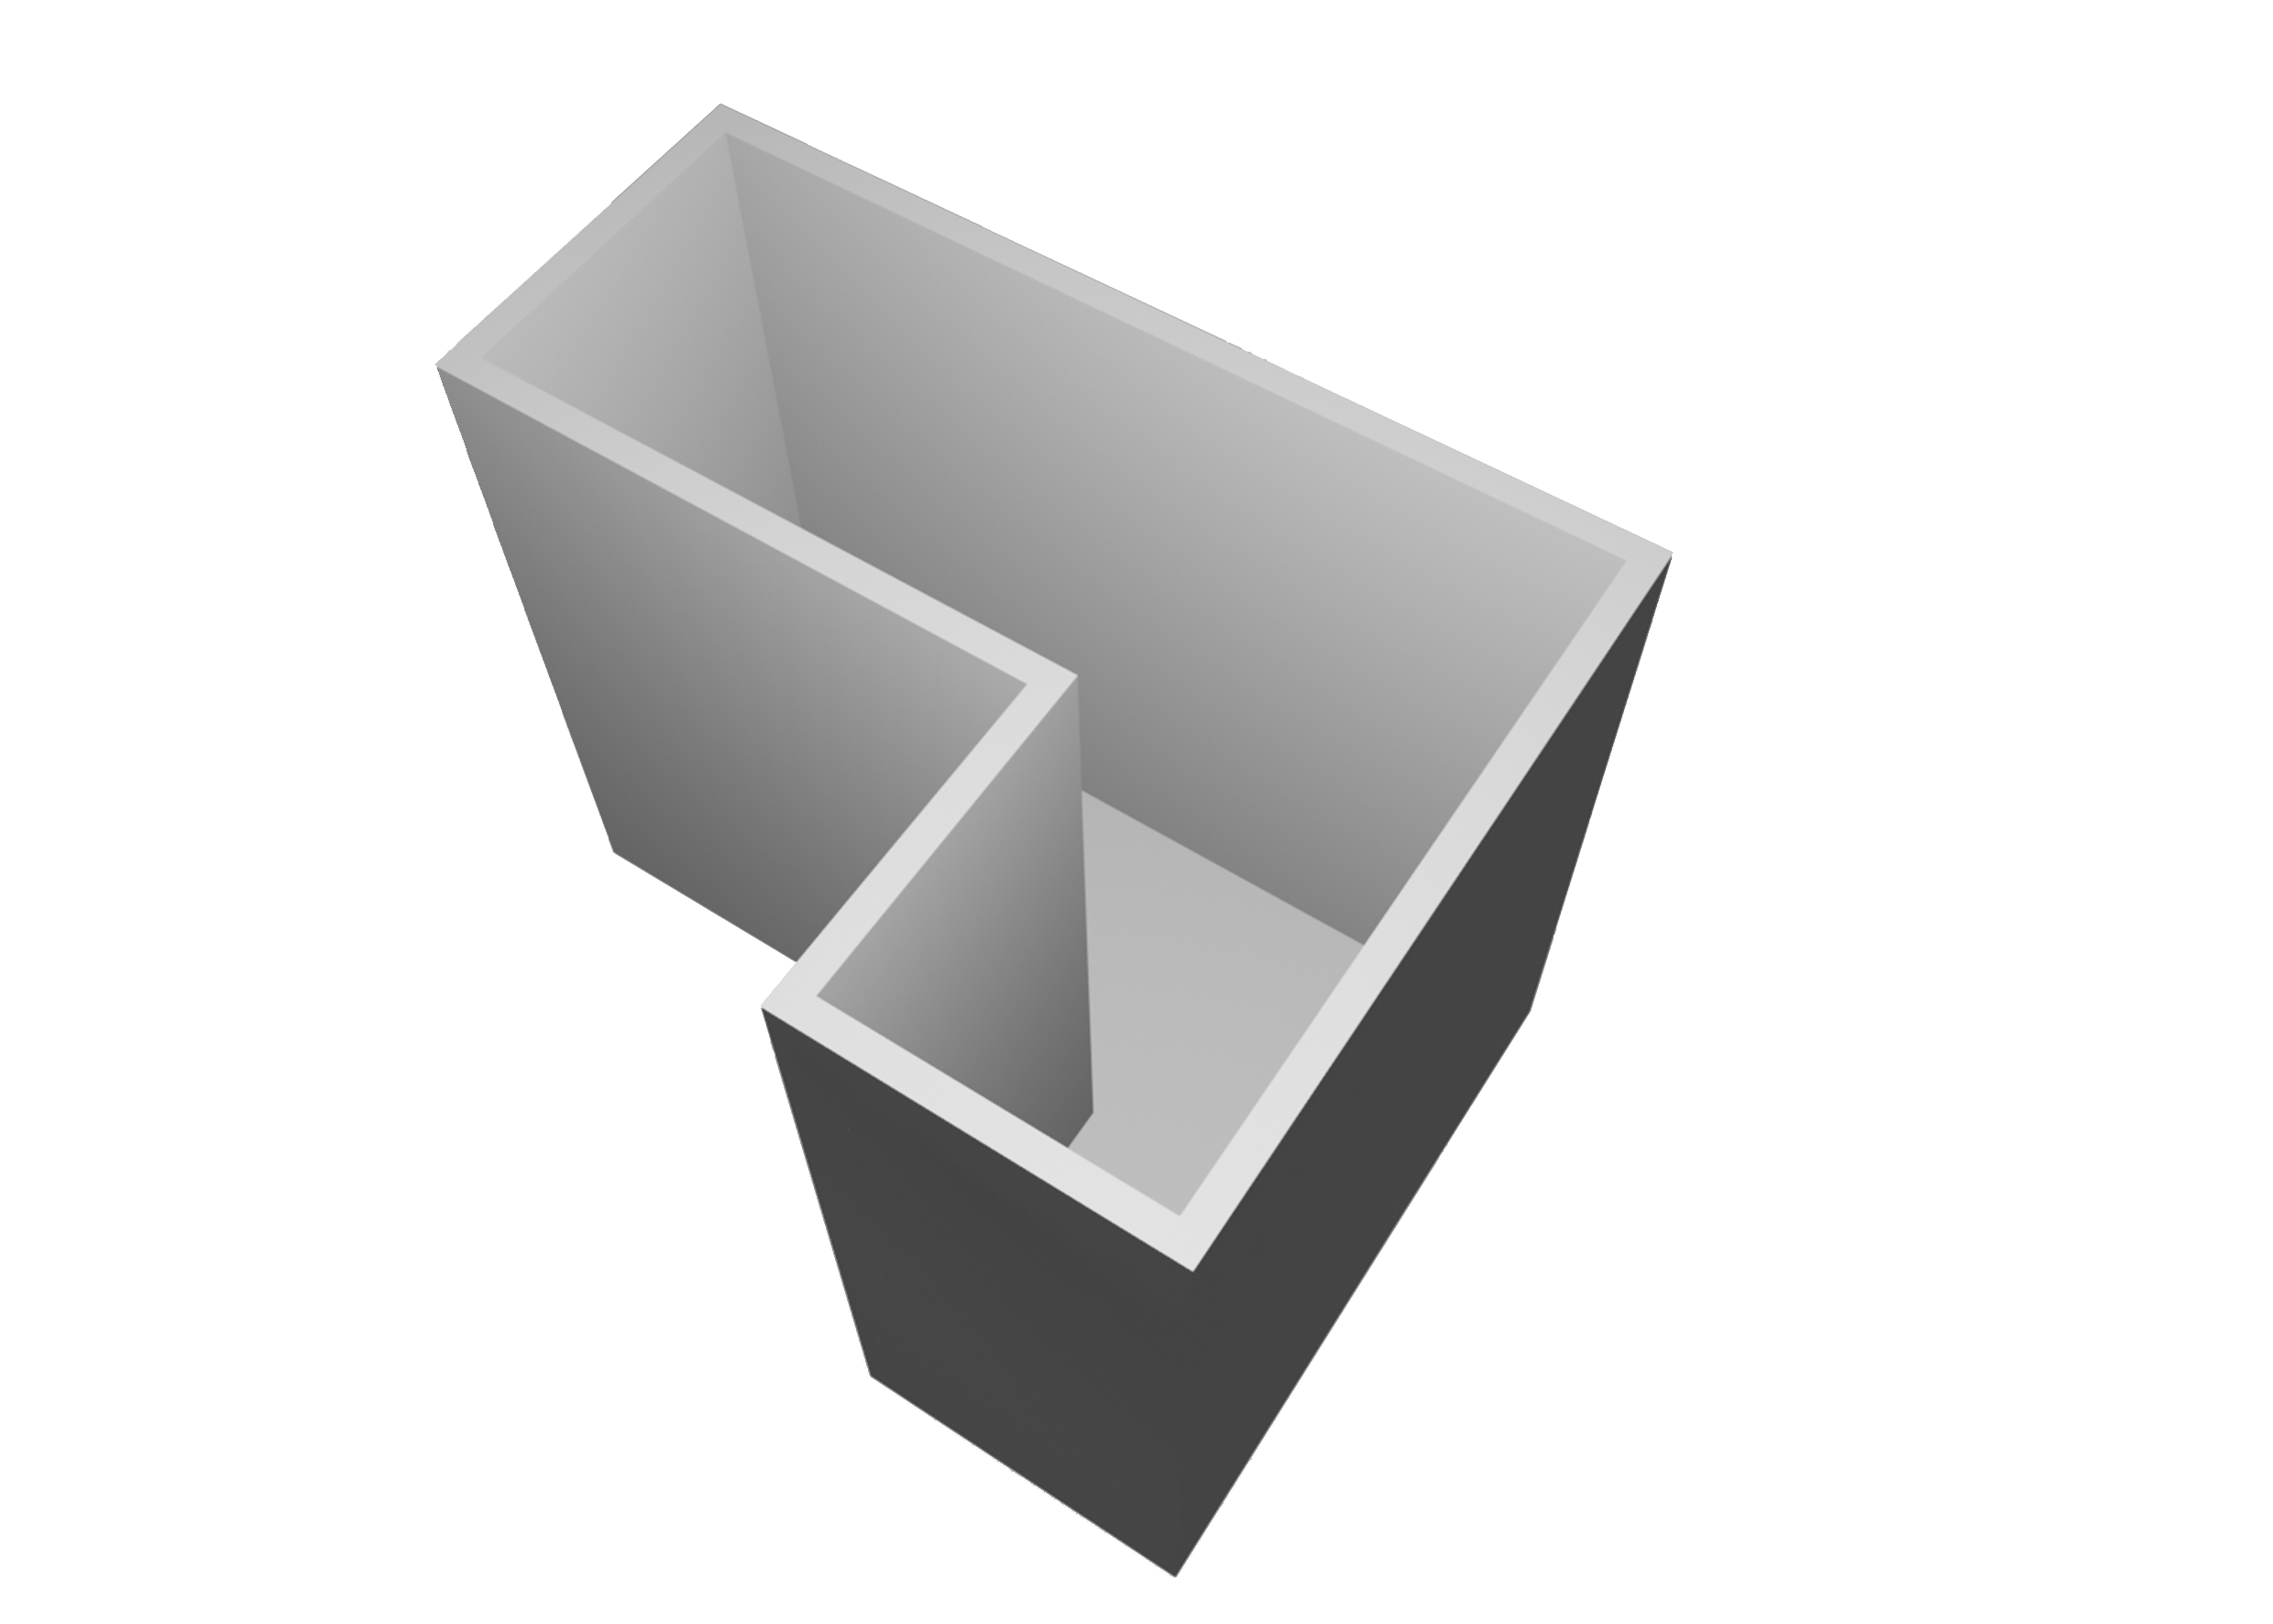
\includegraphics[width=.90\linewidth]{results/pred_2}
	\caption{}
\end{subfigure}
\begin{subfigure}{.49\textwidth}
	\centering
	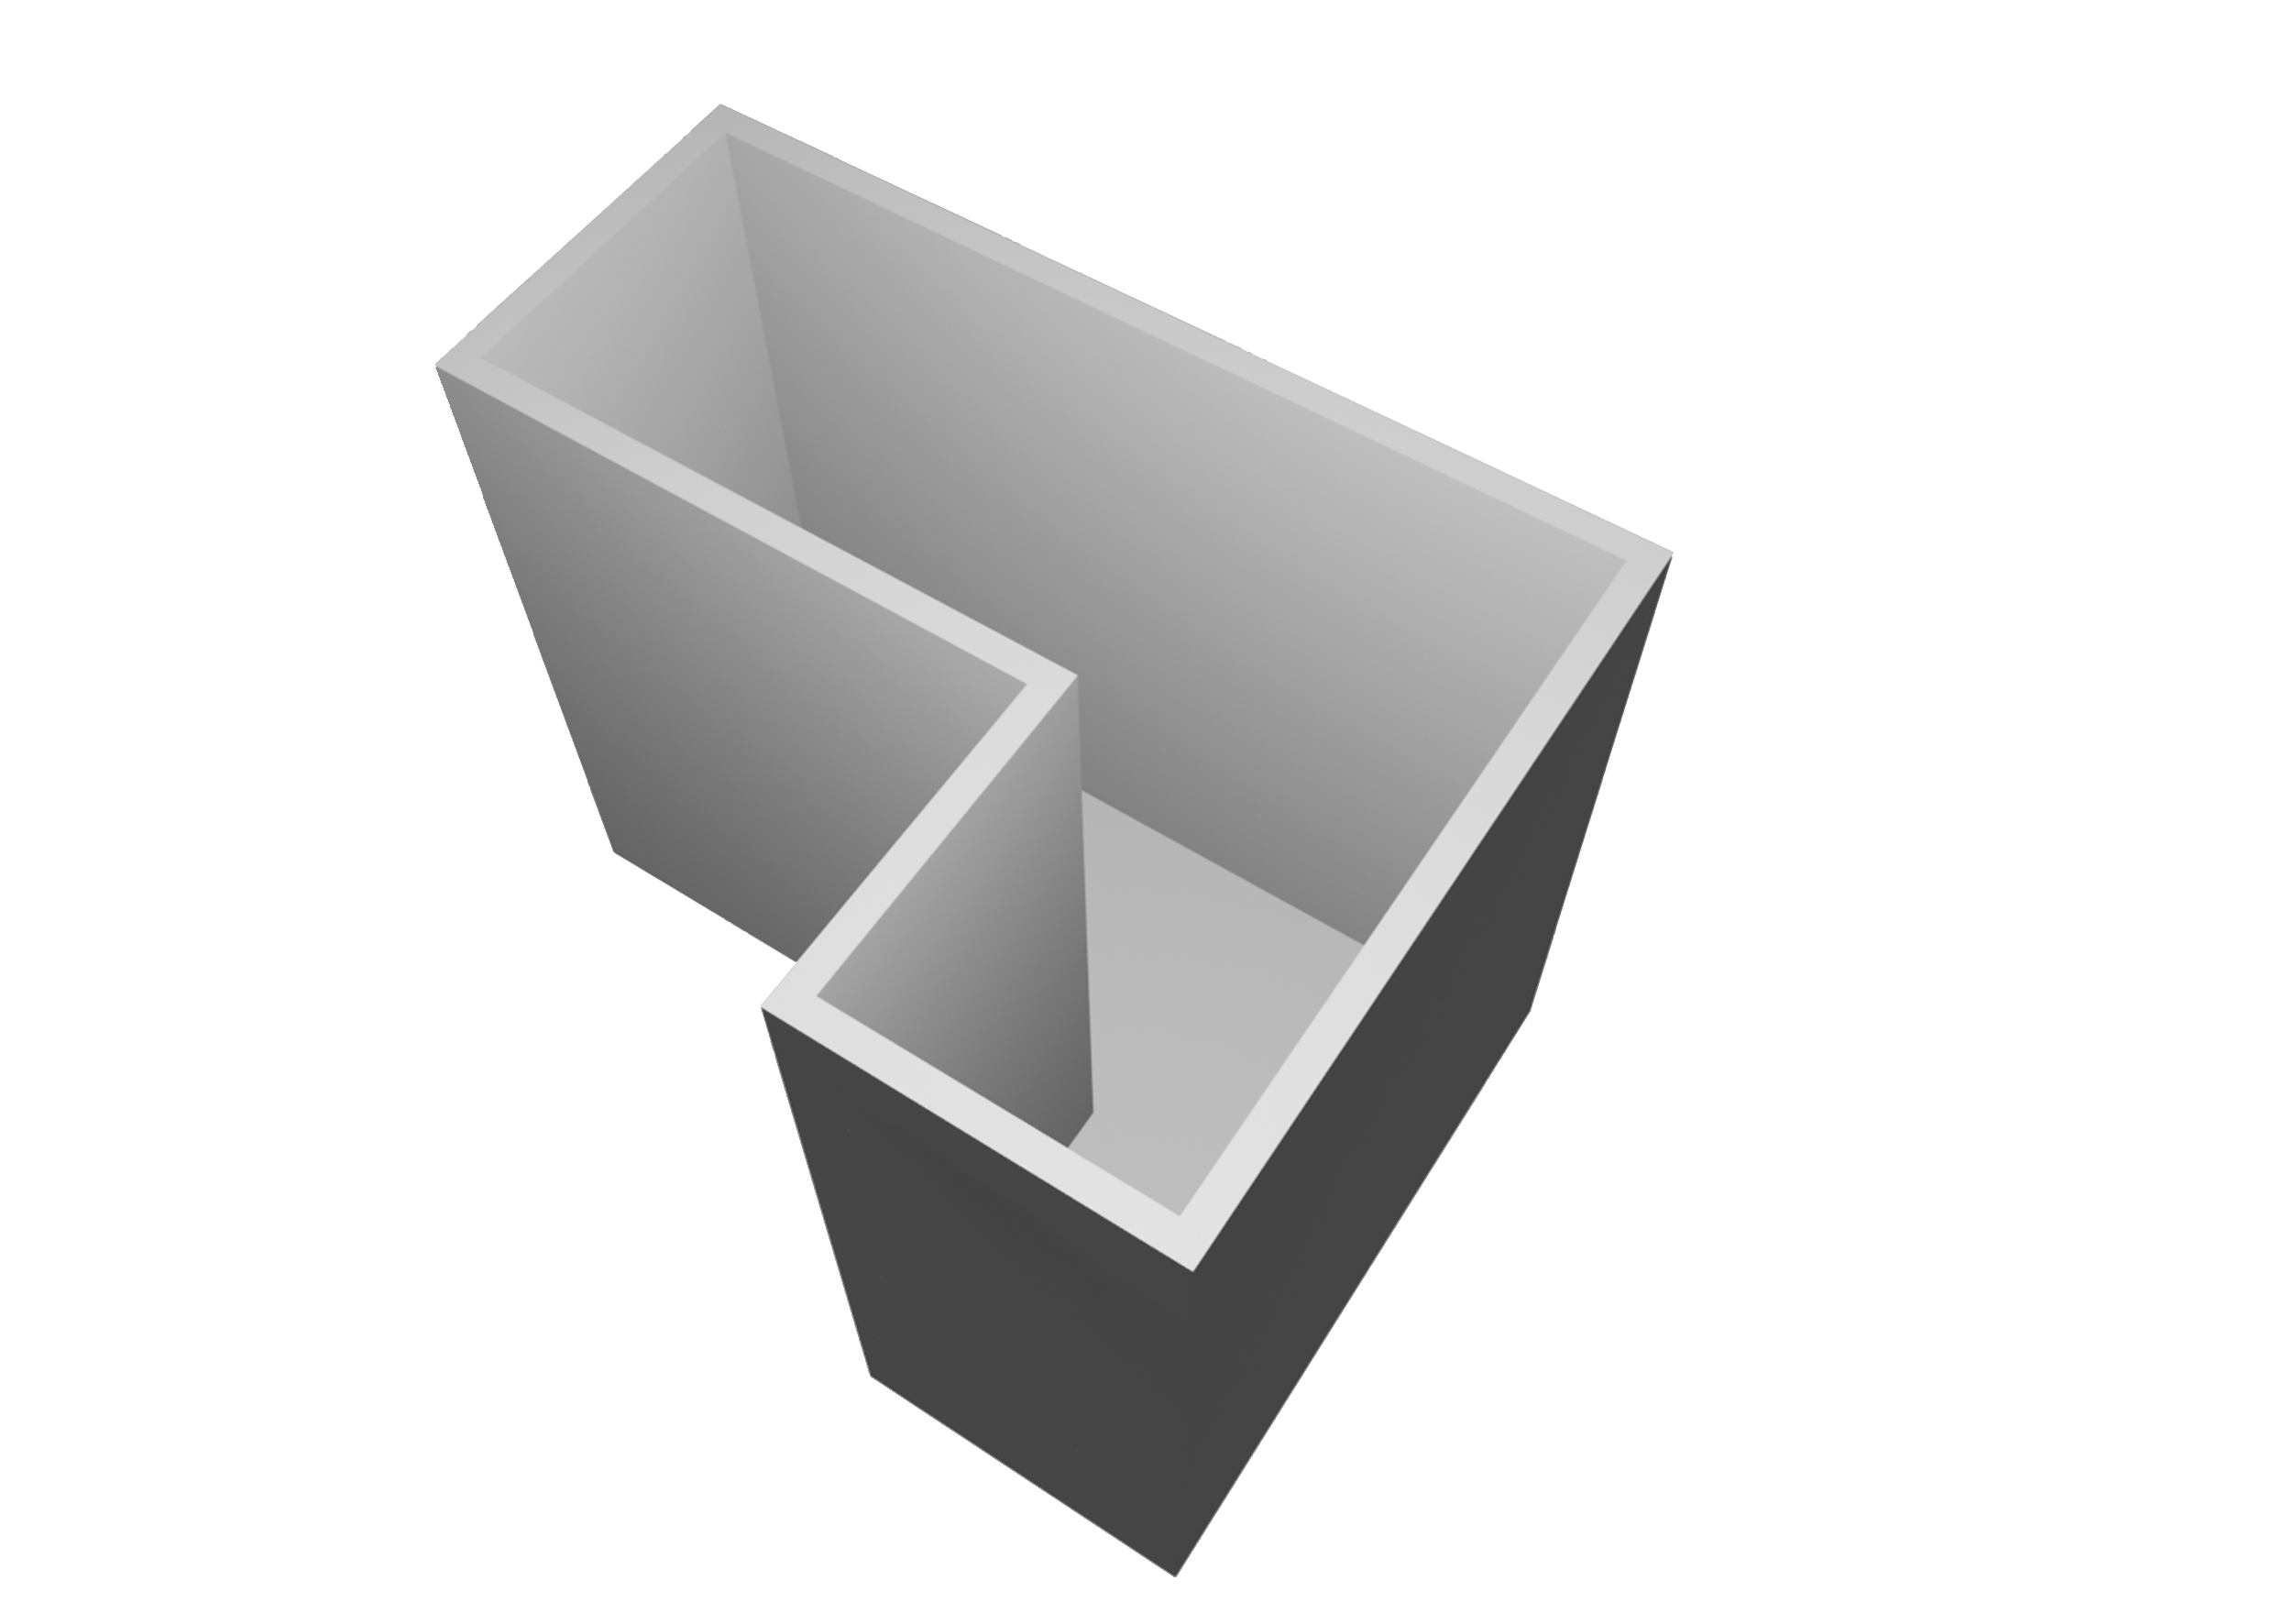
\includegraphics[width=.90\linewidth]{results/true_2}
	\caption{}
\end{subfigure}

\begin{subfigure}{.49\textwidth}
	\centering
	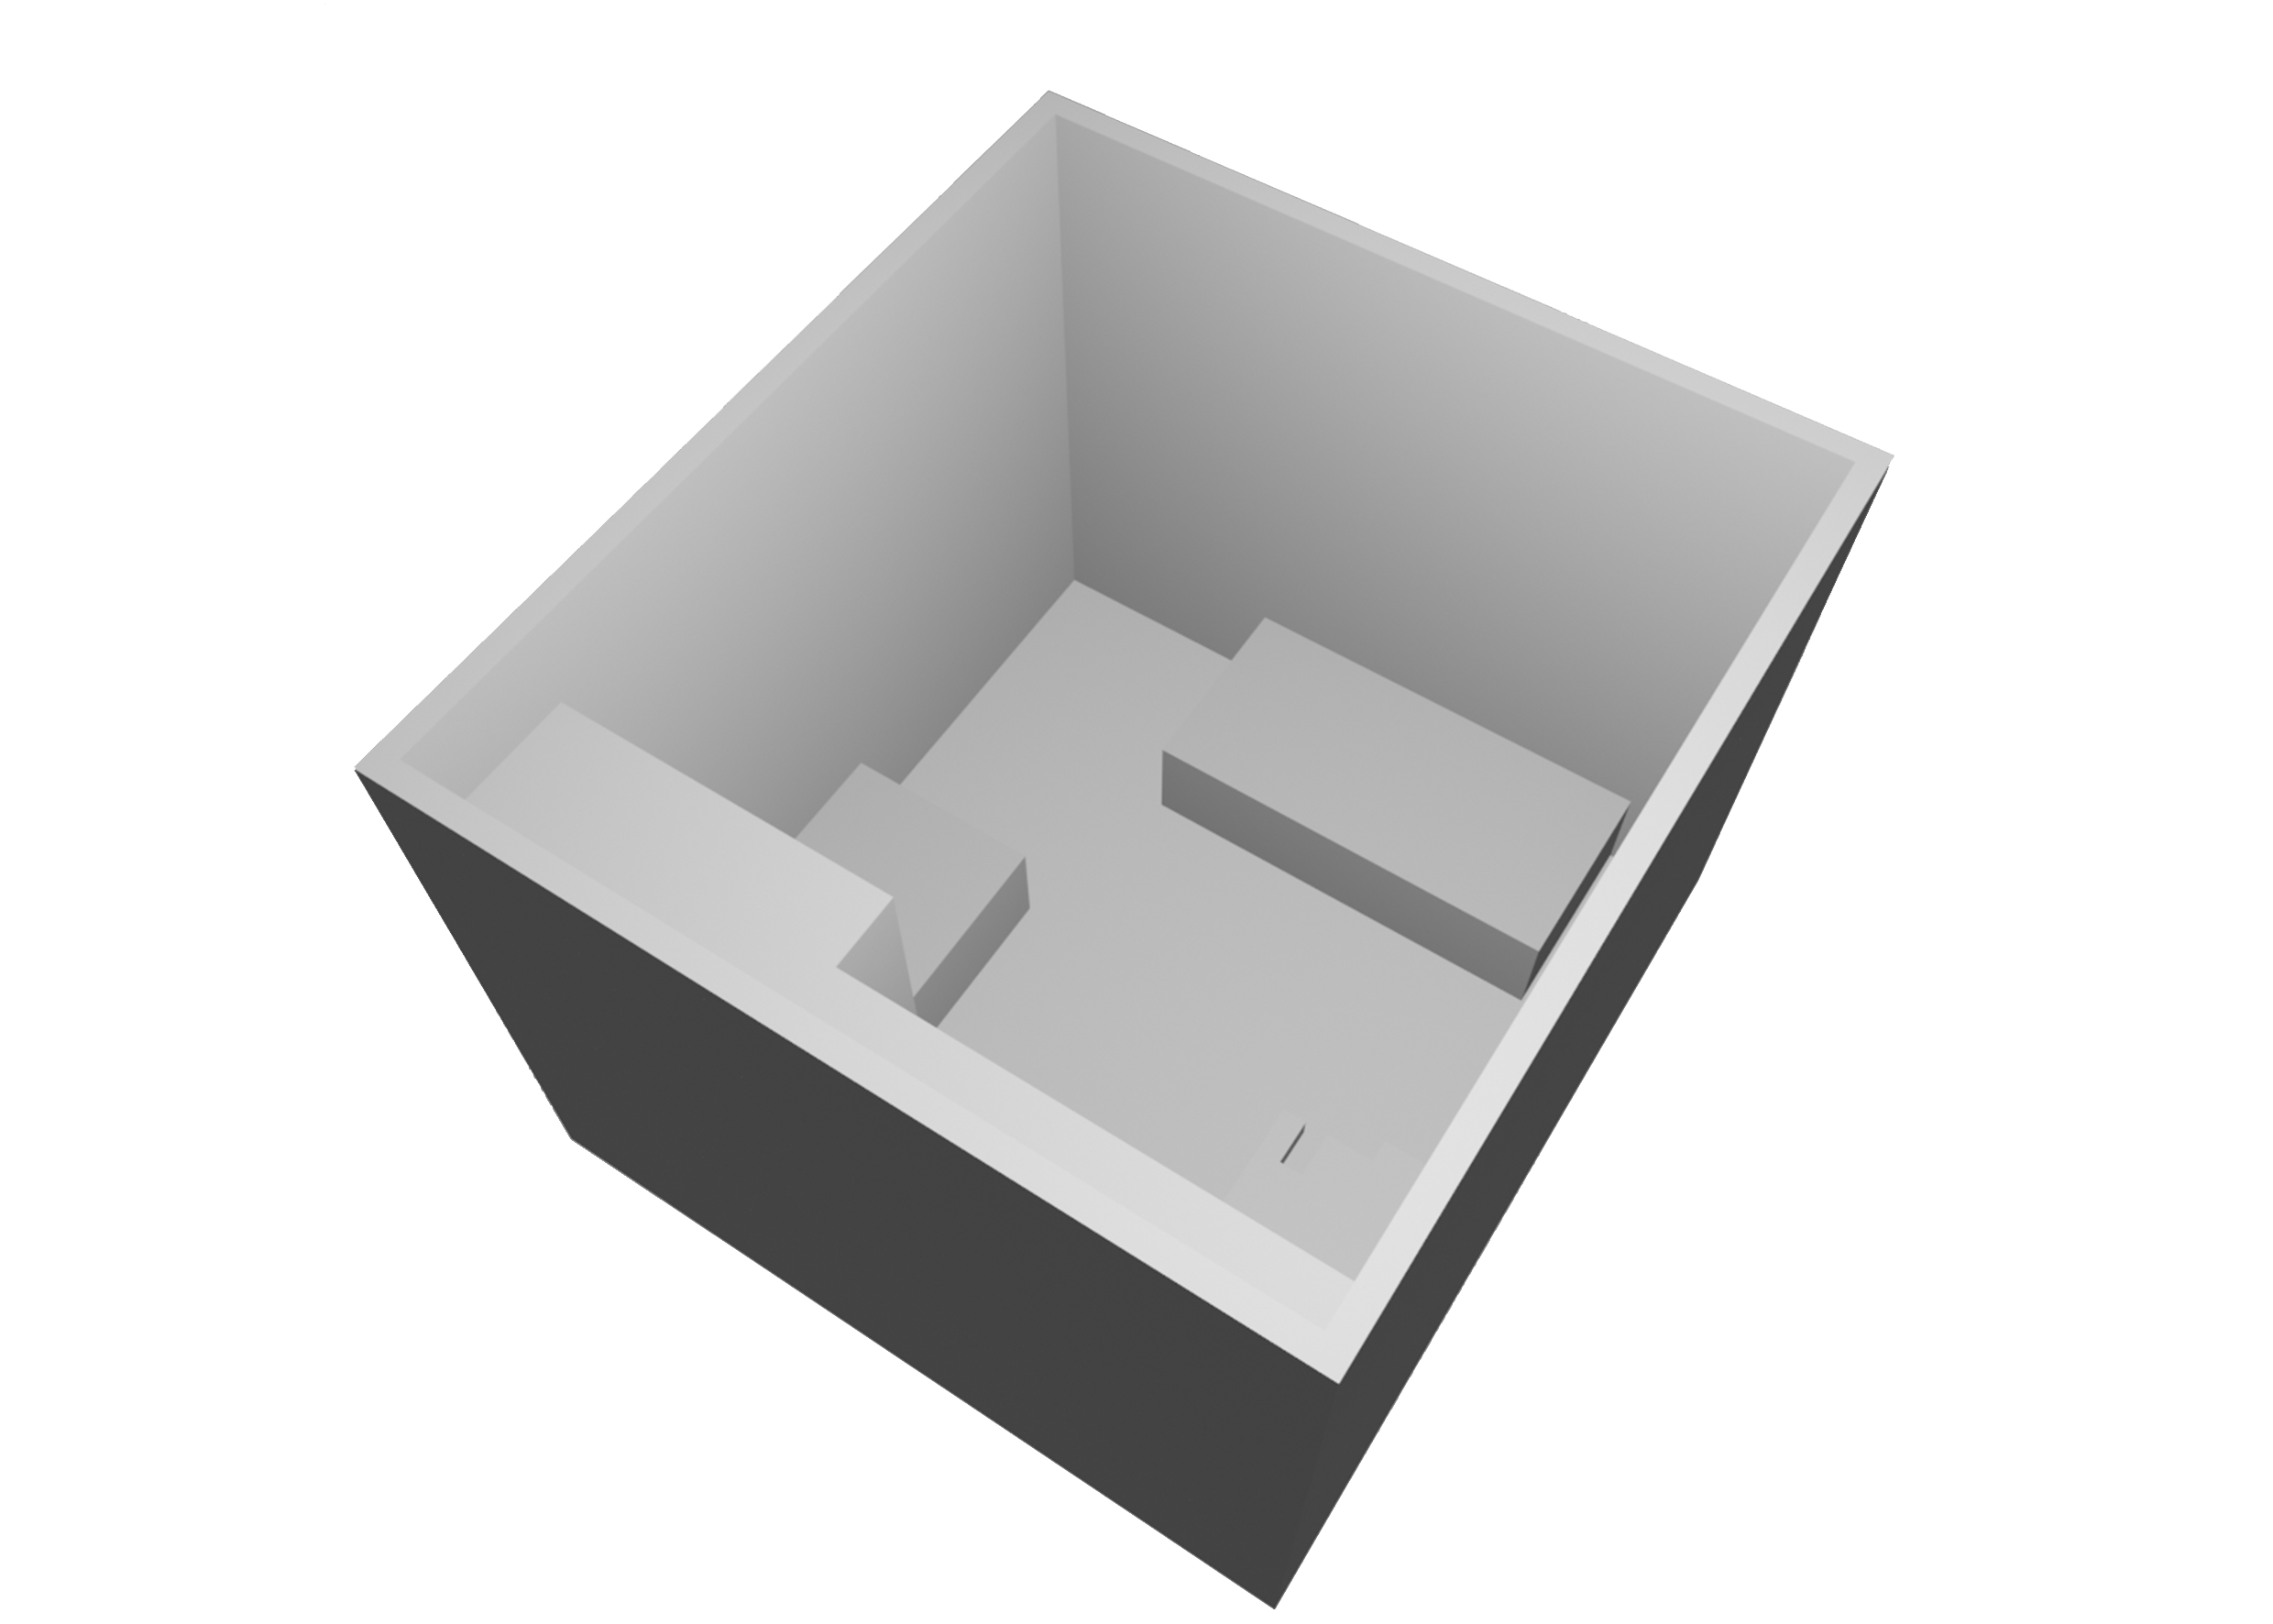
\includegraphics[width=.90\linewidth]{results/pred_3}
	\caption{}
\end{subfigure}
\begin{subfigure}{.49\textwidth}
	\centering
	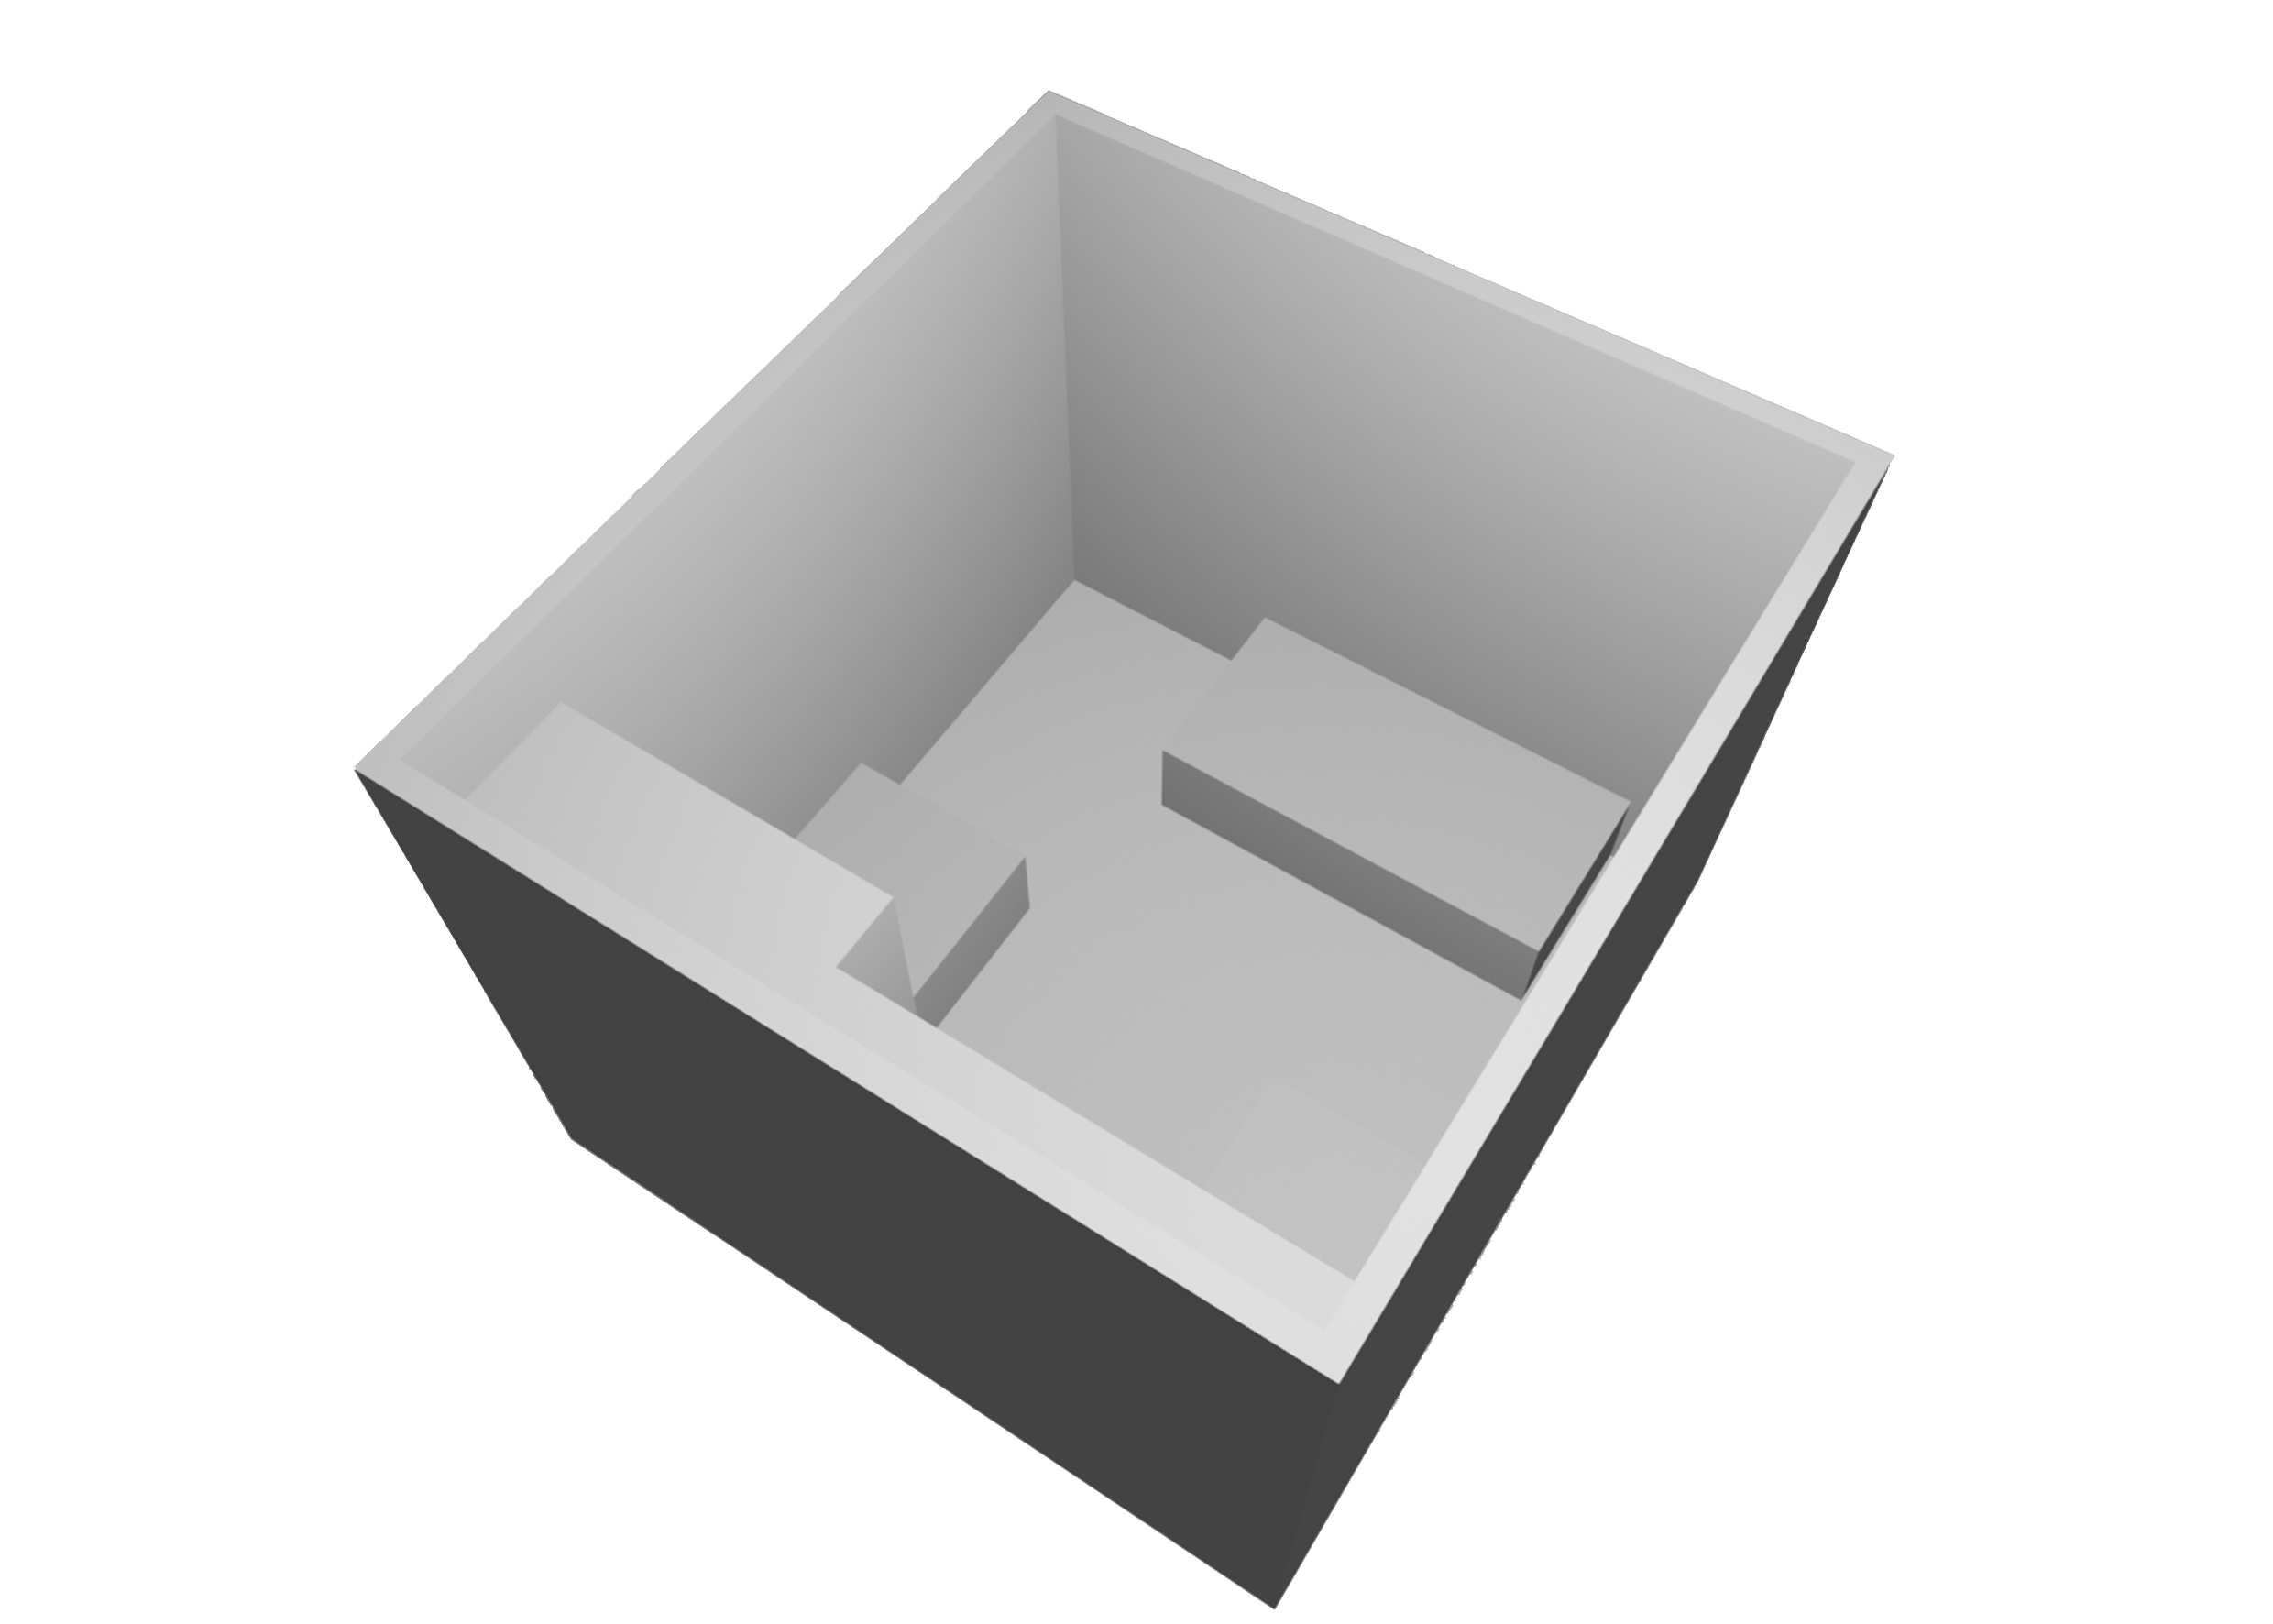
\includegraphics[width=.90\linewidth]{results/true_3}
	\caption{}
\end{subfigure}

\caption{For each row, the first picture is the prediction produced by the proposed method, while the second is the respective ground truth.}
\label{fig:3d-res}
\end{figure}

Since the 3D representations from a single point of view don't allow to present the results in a clear way the same predictions are shown also in a 2D representation from a top view in Figure \ref{fig:2d-res} where the value of the pixel at position $x,z$ is based on the number of voxels with the same $x,z$ position. In detail, the pixel will have an higher value if more voxels have value 1 on the upward axis $y$. Formally, given a voxel grid $Y \in \{0, 1\}^{64 \times 64 \times 64}$ the 2D top view representation $I \in \mathbb{N}^{64 \times 64}$ is determined in the following way:
\begin{equation}
I[x, z] = \sum_{y = 1}^{64} Y[x, y, z].
\end{equation}

\begin{figure}[h!]
\centering
\begin{subfigure}{.49\textwidth}
	\centering
	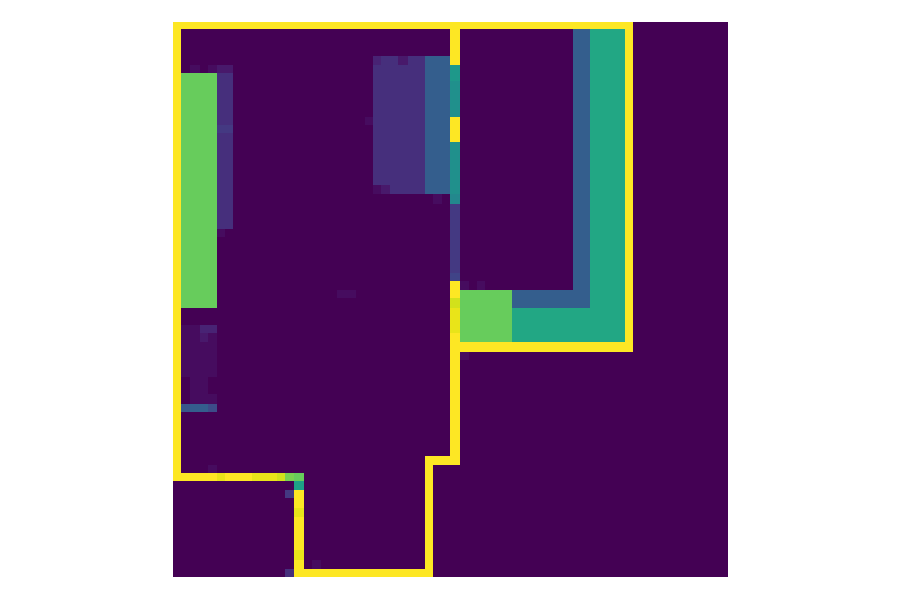
\includegraphics[width=.90\linewidth]{results/top_pred_0}
	\caption{}
\end{subfigure}
\begin{subfigure}{.49\textwidth}
	\centering
	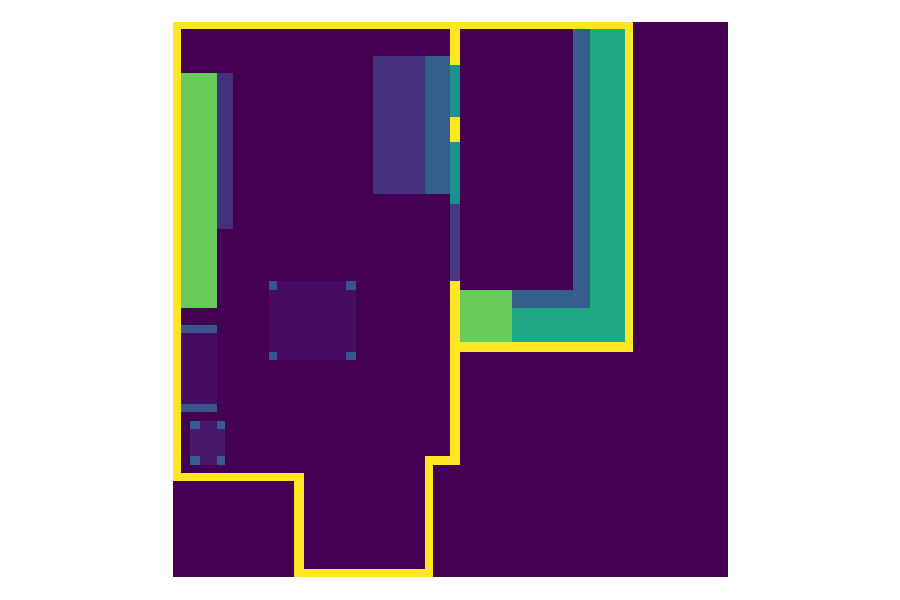
\includegraphics[width=.90\linewidth]{results/top_true_0}
	\caption{}
\end{subfigure}

\begin{subfigure}{.49\textwidth}
	\centering
	
\includegraphics[width=.90\linewidth]{results/top_pred_1}
	\caption{}
\end{subfigure}
\begin{subfigure}{.49\textwidth}
	\centering
	
\includegraphics[width=.90\linewidth]{results/top_true_1}
	\caption{}
\end{subfigure}

\begin{subfigure}{.49\textwidth}
	\centering
	
\includegraphics[width=.90\linewidth]{results/top_pred_2}
	\caption{}
\end{subfigure}
\begin{subfigure}{.49\textwidth}
	\centering
	
\includegraphics[width=.90\linewidth]{results/top_true_2}
	\caption{}
\end{subfigure}

\begin{subfigure}{.49\textwidth}
	\centering
	
\includegraphics[width=.90\linewidth]{results/top_pred_3}
	\caption{}
\end{subfigure}
\begin{subfigure}{.49\textwidth}
	\centering
	
\includegraphics[width=.90\linewidth]{results/top_true_3}
	\caption{}
\end{subfigure}

\caption{Top-view 2D representation of the predictions produced by the proposed method in Figure \ref{fig:3d-res}.}
\label{fig:2d-res}
\end{figure}

From the top-view results we can see better that the model is able to reconstruct almost perfectly the bigger objects inside the rooms, having only difficulties with smaller objects. However, smaller objects have a lower impact on the processed Wi-Fi signal for the physical properties of the signal and therefore limitations regarding the size of the reconstructed objects were expected.


\subsection{Quantitative results}

In order to evaluate the proposed method from a quantitative point of view several metrics were used. The Intersection over Union (IoU) metric is usually used to evaluate how well a predicted mask or bounding box matches the provided ground truth. The IoU is defined in general as the area of overlap over the area of union of the two masks. In the case of voxel grids the IoU can be easily redefined and adapted to the 3D case. In fact, the area of overlap is the number of voxels present in the same positions in both the predicted and ground truth grid, instead the area of union is the total number of voxels present in both grids. Formally, given $\hat{Y}$ as the prediction voxel grid and $Y$ as the associated ground truth we can define the IoU as follows:
\begin{equation}
IoU = \frac{|Y \cap \hat{Y}|}{|Y \cup \hat{Y}|}.
\end{equation}

%\begin{figure}[h!]
%\centering
%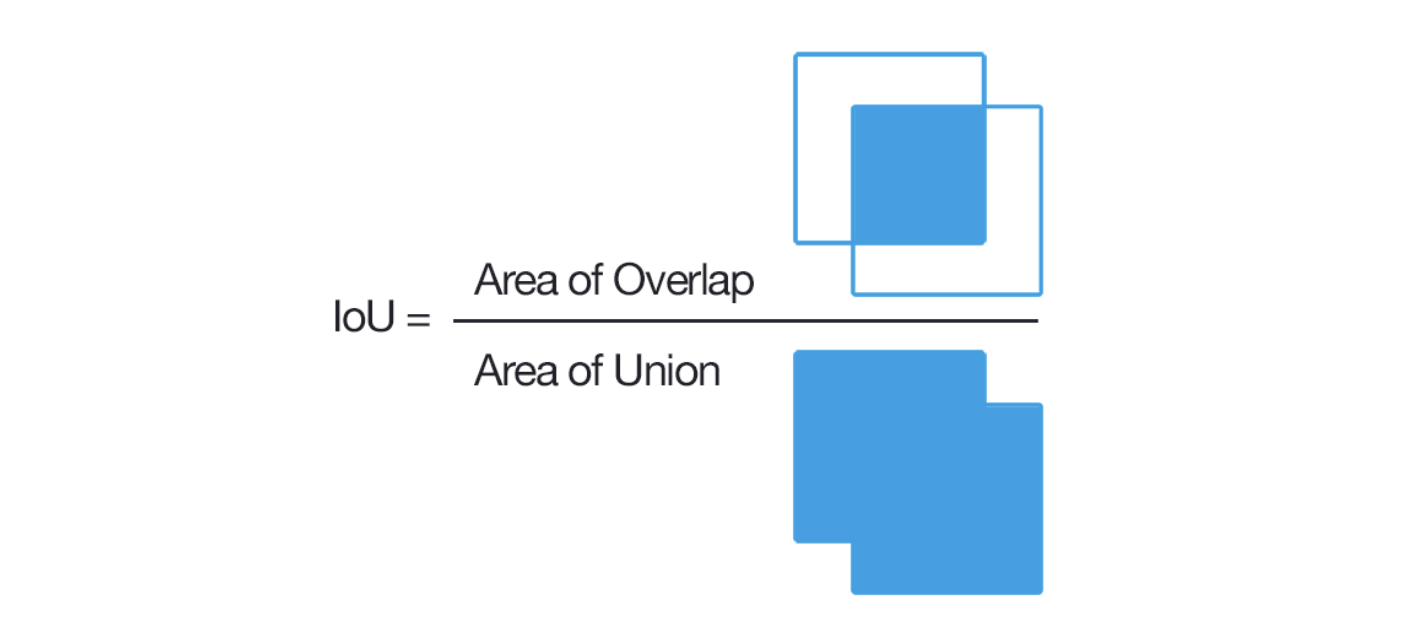
\includegraphics[width=\linewidth]{iou}
%\caption{Intuitive definition of the IoU metric.}
%\label{fig:iou}
%\end{figure}

Moreover, in order to compute the IoU metric the output of the model $\hat{Y}$ needs a simple step of binarization. In fact, the ground truth $Y$ is defined by only zeros and ones, instead the values given in output by the model can also be any number in the interval $[0, 1]$. Therefore, the model output is binarized in the following way:
\begin{equation}
\hat{Y}_b[x, y, z] = \begin{cases}
0 & \text{if } \hat{Y}[x, y, z] \le 0.5 \\
1 & \text{otherwise}
\end{cases}
\end{equation}

In Table \ref{tab:results} the quantitative results for train, validation and test sets are reported using the Dice loss, the Binary Cross-Entropy (BCE) and the Intersection over Union (IoU). The results show that the model is able to obtain an almost perfect score for the IoU on the train set and generalize well at the same time obtaining very high score also on the validation and test sets.

\begin{table}[h!]
\centering
\begin{tabular}{|c|c|c|c|}
\hline
Set & Dice $\downarrow$ & BCE $\downarrow$ & IoU $\uparrow$ \\
\hline\hline
Train & 0.500 & 0.002 & 0.996 \\
\hline
Validate & 0.514 & 0.023 & 0.958 \\
\hline
Test & 0.509 & 0.012 & 0.971 \\
\hline
\end{tabular}
\caption{Table evaluating the results obtained by the proposed method using the Dice loss, Binary Cross-Entropy (BCE) and Intersection over Union (IoU) for train, validate and test set.}
\label{tab:results}
\end{table}

Moreover, in Figures \ref{fig:dice} and \ref{fig:iou} are shown respectively the dice loss and IoU metric computed during training on the train and validate set at each epoch. The plots show that the training is performed smoothly until reaching the convergence of the loss, which is at around 0.5. Moreover, as we can see from the validation values, the model doesn't have any of the classical signs of overfitting in which the training loss continues to decrease but the validation loss increases.

\begin{figure}[h!]
\centering
\includegraphics[width=\linewidth]{dice-plot}
\caption{Plot of the dice loss computed on the train and validate set during training.}
\label{fig:dice}
\end{figure}

\begin{figure}[h!]
\centering
\includegraphics[width=\linewidth]{iou-plot}
\caption{Plot of the IoU metric computed on the train and validate set during training.}
\label{fig:iou}
\end{figure}

\section{Ablation studies}\label{sec:ablation}

This work cannot be compared with the state of the art as usual since there aren't other works in the literature that address a similar task. Therefore, more in-depth ablation studies will be performed analyzing the impact of the loss, providing as input amplitude and phase, varying linear projection dimensions and number of packets. In Table \ref{tab:loss-abl-stu} is shown the IoU computed on the test set training the model using the Binary Cross-Entropy (BCE) and the Dice loss. From the results we can see that the Dice loss is marginally better than the BCE, therefore all the other ablation studies have been done training the model with this loss.

\begin{table}[h!]
\centering
\begin{tabular}{|c|c|>{\centering\arraybackslash}p{.2\textwidth}|}
\hline
\multicolumn{2}{|c|}{\textbf{Loss}} & \textbf{IoU} \\
\hline
\multicolumn{2}{|c|}{BCE} & 0.967 \\
\hline
\multicolumn{2}{|c|}{Dice} & \textbf{0.971} \\
\hline
\end{tabular}
\caption{Table reporting the best IoU for the ablation studies regarding the loss.}
\label{tab:loss-abl-stu}
\end{table}

Instead in Table \ref{tab:abl-stu} the results for all the other ablation studies are reported. The results on the input of the model show that both amplitude and phase carries some information about the environment. As expected, the amplitude is the signal component which has more impact for the reconstruction of the environment but also the phase seems to be useful for this task.
Continuing, the experiments on the embedding dimension for the linear projection before the encoder $E$ and before the decoder $D$ show that even with different combinations we can obtain good results. For small values, like $E=32$ $D=32$, the model is able to reach good IoU on the test set but it is not able to reach the maximum score since it is probably limited by the size of the encoding which makes the task harder. Instead, on the other hand, higher values, like $E=128$ $D=128$, may produce sparser representation, adding only not useful information and lowering the accuracy by consequence. Therefore, the perfect spot seems to be very close to the initial dimension of the subcarriers, i.e. $K = 50$.
Finally, as we can notice inspecting the dataset, the information contained in the different packets doesn't change much during the collection, in fact the environment is static and no movement is recorded during the sessions. Thus, the number of packets used by the model to produce the predictions doesn't affect too much the results since the values of different packets for the same subcarrier are very close to each other.

\begin{table}[h!]
\centering
\begin{tabular}{|c|c|>{\centering\arraybackslash}p{.2\textwidth}|}
\hline
\multicolumn{2}{|c|}{\textbf{Input}} & \textbf{IoU} \\
\hline
\multicolumn{2}{|c|}{Amplitude} & 0.904 \\
\hline
\multicolumn{2}{|c|}{Phase} & 0.881 \\
\hline
\multicolumn{2}{|c|}{Amplitude and Phase} & \textbf{0.971} \\
\hline\hline
\textbf{Encoder dim ($E$)} & \textbf{Decoder dim ($D$)} & \textbf{IoU} \\
\hline
32 & 32 & 0.903 \\
\hline
32 & 64 & 0.936 \\
\hline
64 & 32 & 0.967 \\
\hline
64 & 64 & \textbf{0.971} \\
\hline
128 & 64 & 0.964 \\
\hline
64 & 128 & 0.926 \\
\hline
128 & 128 & 0.921 \\
\hline\hline
\multicolumn{2}{|c|}{\textbf{Number of packets ($P$)}} & \textbf{IoU} \\
\hline
\multicolumn{2}{|c|}{32} & 0.948 \\
\hline
\multicolumn{2}{|c|}{64} & \textbf{0.971} \\
\hline
\multicolumn{2}{|c|}{128} & 0.930 \\
\hline
\end{tabular}
\caption{Table reporting the best IoU for the ablation studies computed using the Dice loss.}
\label{tab:abl-stu}
\end{table}


\chapter{Conclusions}\label{cap:conclusions}

This thesis presented the first work which aims to perform 3D indoor environment reconstruction using Wi-Fi sensing. A novel dataset was collected in order to train a model in order to present a first solution for this task. The proposed method is based on a sanitization procedure on both amplitude and phase on the collected data and a transformer-based architecture for the deep model. The results produced by the proposed architecture has been validated both from a qualitative and quantitative point of view, showing how the CSI data can actually carry enough information to discriminate and reconstruct environments.

Several in-depth ablation studies were performed, which showed the impact of the dice loss with respect to the binary cross-entropy, the embedding dimensions to fed respectively to encoder and decoder and the number of packets. However, the major result of the ablation studies was regarding the input. In fact, the proposed method was evaluated with only amplitude, only phase and both amplitude and phase data. The results showed how the phase is the signal component which carries less information about the environment but used in conjunction with the amplitude can provide the best results.

As future work, the dataset could be augmented in order to provide even more samples of several rooms. 
Moreover, it is possible to study and experiment about the details of the reconstructions since this work used voxels with a fixed unit of 10 cm, which implies that any objects or detail in the room smaller than this size will not be reproduced by the model. Thus, more experiments in future can be carried out with a smaller voxel unit and hopefully more detailed reconstructions can be produced. On the other hand, instead of the voxel space used in this work, completely different representations of the environments could be used, like triangular meshes or point clouds.

In the end, regarding the method, this work considers the walls and the objects in the room in the same way, while another approach could be investigated in which single objects are reconstructed independently from the walls of the room.


\backmatter
\cleardoublepage
\phantomsection % Give this command only if hyperref is loaded
\addcontentsline{toc}{chapter}{\bibname}
% Here put the code for the bibliography. You can use BibTeX or
% the BibLaTeX package or the simple environment thebibliography.
\bibliographystyle{sapthesis} % BibTeX style
\bibliography{bibliography}

\end{document}